% Options for packages loaded elsewhere
\PassOptionsToPackage{unicode}{hyperref}
\PassOptionsToPackage{hyphens}{url}
%
\documentclass[
]{book}
\usepackage{amsmath,amssymb}
\usepackage{iftex}
\ifPDFTeX
  \usepackage[T1]{fontenc}
  \usepackage[utf8]{inputenc}
  \usepackage{textcomp} % provide euro and other symbols
\else % if luatex or xetex
  \usepackage{unicode-math} % this also loads fontspec
  \defaultfontfeatures{Scale=MatchLowercase}
  \defaultfontfeatures[\rmfamily]{Ligatures=TeX,Scale=1}
\fi
\usepackage{lmodern}
\ifPDFTeX\else
  % xetex/luatex font selection
\fi
% Use upquote if available, for straight quotes in verbatim environments
\IfFileExists{upquote.sty}{\usepackage{upquote}}{}
\IfFileExists{microtype.sty}{% use microtype if available
  \usepackage[]{microtype}
  \UseMicrotypeSet[protrusion]{basicmath} % disable protrusion for tt fonts
}{}
\makeatletter
\@ifundefined{KOMAClassName}{% if non-KOMA class
  \IfFileExists{parskip.sty}{%
    \usepackage{parskip}
  }{% else
    \setlength{\parindent}{0pt}
    \setlength{\parskip}{6pt plus 2pt minus 1pt}}
}{% if KOMA class
  \KOMAoptions{parskip=half}}
\makeatother
\usepackage{xcolor}
\usepackage{color}
\usepackage{fancyvrb}
\newcommand{\VerbBar}{|}
\newcommand{\VERB}{\Verb[commandchars=\\\{\}]}
\DefineVerbatimEnvironment{Highlighting}{Verbatim}{commandchars=\\\{\}}
% Add ',fontsize=\small' for more characters per line
\usepackage{framed}
\definecolor{shadecolor}{RGB}{248,248,248}
\newenvironment{Shaded}{\begin{snugshade}}{\end{snugshade}}
\newcommand{\AlertTok}[1]{\textcolor[rgb]{0.94,0.16,0.16}{#1}}
\newcommand{\AnnotationTok}[1]{\textcolor[rgb]{0.56,0.35,0.01}{\textbf{\textit{#1}}}}
\newcommand{\AttributeTok}[1]{\textcolor[rgb]{0.13,0.29,0.53}{#1}}
\newcommand{\BaseNTok}[1]{\textcolor[rgb]{0.00,0.00,0.81}{#1}}
\newcommand{\BuiltInTok}[1]{#1}
\newcommand{\CharTok}[1]{\textcolor[rgb]{0.31,0.60,0.02}{#1}}
\newcommand{\CommentTok}[1]{\textcolor[rgb]{0.56,0.35,0.01}{\textit{#1}}}
\newcommand{\CommentVarTok}[1]{\textcolor[rgb]{0.56,0.35,0.01}{\textbf{\textit{#1}}}}
\newcommand{\ConstantTok}[1]{\textcolor[rgb]{0.56,0.35,0.01}{#1}}
\newcommand{\ControlFlowTok}[1]{\textcolor[rgb]{0.13,0.29,0.53}{\textbf{#1}}}
\newcommand{\DataTypeTok}[1]{\textcolor[rgb]{0.13,0.29,0.53}{#1}}
\newcommand{\DecValTok}[1]{\textcolor[rgb]{0.00,0.00,0.81}{#1}}
\newcommand{\DocumentationTok}[1]{\textcolor[rgb]{0.56,0.35,0.01}{\textbf{\textit{#1}}}}
\newcommand{\ErrorTok}[1]{\textcolor[rgb]{0.64,0.00,0.00}{\textbf{#1}}}
\newcommand{\ExtensionTok}[1]{#1}
\newcommand{\FloatTok}[1]{\textcolor[rgb]{0.00,0.00,0.81}{#1}}
\newcommand{\FunctionTok}[1]{\textcolor[rgb]{0.13,0.29,0.53}{\textbf{#1}}}
\newcommand{\ImportTok}[1]{#1}
\newcommand{\InformationTok}[1]{\textcolor[rgb]{0.56,0.35,0.01}{\textbf{\textit{#1}}}}
\newcommand{\KeywordTok}[1]{\textcolor[rgb]{0.13,0.29,0.53}{\textbf{#1}}}
\newcommand{\NormalTok}[1]{#1}
\newcommand{\OperatorTok}[1]{\textcolor[rgb]{0.81,0.36,0.00}{\textbf{#1}}}
\newcommand{\OtherTok}[1]{\textcolor[rgb]{0.56,0.35,0.01}{#1}}
\newcommand{\PreprocessorTok}[1]{\textcolor[rgb]{0.56,0.35,0.01}{\textit{#1}}}
\newcommand{\RegionMarkerTok}[1]{#1}
\newcommand{\SpecialCharTok}[1]{\textcolor[rgb]{0.81,0.36,0.00}{\textbf{#1}}}
\newcommand{\SpecialStringTok}[1]{\textcolor[rgb]{0.31,0.60,0.02}{#1}}
\newcommand{\StringTok}[1]{\textcolor[rgb]{0.31,0.60,0.02}{#1}}
\newcommand{\VariableTok}[1]{\textcolor[rgb]{0.00,0.00,0.00}{#1}}
\newcommand{\VerbatimStringTok}[1]{\textcolor[rgb]{0.31,0.60,0.02}{#1}}
\newcommand{\WarningTok}[1]{\textcolor[rgb]{0.56,0.35,0.01}{\textbf{\textit{#1}}}}
\usepackage{longtable,booktabs,array}
\usepackage{calc} % for calculating minipage widths
% Correct order of tables after \paragraph or \subparagraph
\usepackage{etoolbox}
\makeatletter
\patchcmd\longtable{\par}{\if@noskipsec\mbox{}\fi\par}{}{}
\makeatother
% Allow footnotes in longtable head/foot
\IfFileExists{footnotehyper.sty}{\usepackage{footnotehyper}}{\usepackage{footnote}}
\makesavenoteenv{longtable}
\usepackage{graphicx}
\makeatletter
\def\maxwidth{\ifdim\Gin@nat@width>\linewidth\linewidth\else\Gin@nat@width\fi}
\def\maxheight{\ifdim\Gin@nat@height>\textheight\textheight\else\Gin@nat@height\fi}
\makeatother
% Scale images if necessary, so that they will not overflow the page
% margins by default, and it is still possible to overwrite the defaults
% using explicit options in \includegraphics[width, height, ...]{}
\setkeys{Gin}{width=\maxwidth,height=\maxheight,keepaspectratio}
% Set default figure placement to htbp
\makeatletter
\def\fps@figure{htbp}
\makeatother
\usepackage{soul}
\setlength{\emergencystretch}{3em} % prevent overfull lines
\providecommand{\tightlist}{%
  \setlength{\itemsep}{0pt}\setlength{\parskip}{0pt}}
\setcounter{secnumdepth}{5}
\usepackage{booktabs}
\ifLuaTeX
  \usepackage{selnolig}  % disable illegal ligatures
\fi
\usepackage[]{natbib}
\bibliographystyle{apalike}
\IfFileExists{bookmark.sty}{\usepackage{bookmark}}{\usepackage{hyperref}}
\IfFileExists{xurl.sty}{\usepackage{xurl}}{} % add URL line breaks if available
\urlstyle{same}
\hypersetup{
  pdftitle={A Beginner's Guide to Systematic Review and Meta-Analysis},
  pdfauthor={Noah L. Schroeder, Ph.D.},
  hidelinks,
  pdfcreator={LaTeX via pandoc}}

\title{A Beginner's Guide to Systematic Review and Meta-Analysis}
\author{Noah L. Schroeder, Ph.D.}
\date{2024-02-06}

\begin{document}
\maketitle

{
\setcounter{tocdepth}{1}
\tableofcontents
}
\hypertarget{welcome}{%
\chapter*{Welcome}\label{welcome}}
\addcontentsline{toc}{chapter}{Welcome}

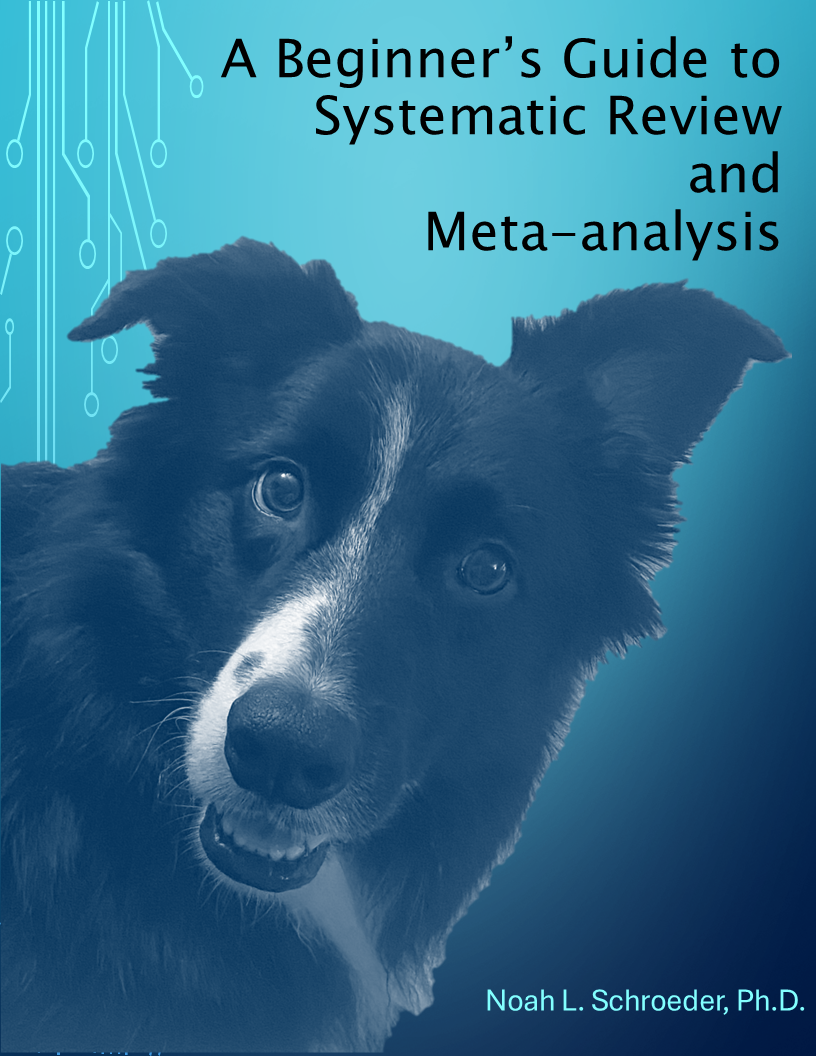
\includegraphics[width=0.5\textwidth,height=\textheight]{images/cover.png}

This book is designed as a fundamental ``how-to'' guide to help researchers new to systematic review and meta-analysis in education and other fields. \ul{This book is focused on how to execute these methodologies, not the statistics driving specific methods}. It is written in a rather informal format in an effort to help a reader connect with the content.

While following the steps in this book can help you run a systematic review or meta-analysis successfully, I highly recommend learning why certain decisions are made. For example, in the meta-analysis section of this book, I assume that you understand what is happening statistically in a meta-analysis. I do not explain the formulas, main ideas, assumptions, etc. in any sort of depth. There are plenty of resources available to help you learn this information, it is simply outside the current scope of this book. \ul{This book is currently a strictly a ``how-to'' guide and I have no intention to make it into what I would consider a ``true'' statistics book.}

\textbf{What makes this book different than others?} All meta-analysis examples in this book are using standardized mean difference effect sizes (Hedge's \emph{g}). There are a lot of examples online of meta-analysis in R using correlations, and this book was created, in part, because there were very few resources I could find about how to do meta-analysis with standardized mean differences.

\hypertarget{what-standards-and-packages-does-this-book-align-with}{%
\section*{What standards and packages does this book align with?}\label{what-standards-and-packages-does-this-book-align-with}}
\addcontentsline{toc}{section}{What standards and packages does this book align with?}

I provide guidance in relation to the \href{http://www.prisma-statement.org/}{PRISMA guidelines} \citep{page2021} and we will use \href{http://www.metafor-project.org/doku.php/metafor}{metafor} \citep{viechtbauer2010} (and other packages) for conducting meta-analyses.

\hypertarget{who-is-this-book-for}{%
\section*{Who is this book for?}\label{who-is-this-book-for}}
\addcontentsline{toc}{section}{Who is this book for?}

This book is designed for:

\begin{itemize}
\item
  People who are just learning about systematic review and meta-analysis methods.
\item
  People who understand meta-analysis, but I don't really understand R.
\item
  People who are used to using graphic user interface (GUI)-based programs for conducting meta-analysis, but want to switch to R.
\item
  Anyone else who wants to improve their knowledge of systematic review and meta-analytical methods.
\end{itemize}

My aim with this book is to make systematic review, and particularly meta-analysis, accessible to those who may not fully understand every aspect of R, want to create reproducible analyses, and most of all, enjoy the free nature of R.

\hypertarget{what-will-you-learn}{%
\section*{What will you learn?}\label{what-will-you-learn}}
\addcontentsline{toc}{section}{What will you learn?}

After reading this book, you will be able to:

\begin{itemize}
\item
  establish research questions and inclusion criteria
\item
  conduct a well-documented literature search
\item
  screen abstracts and studies
\item
  conduct a conventional meta-analysis in R
\item
  conduct a three-level meta-analysis in R
\end{itemize}

\hypertarget{why-does-this-book-exist}{%
\section*{Why does this book exist?}\label{why-does-this-book-exist}}
\addcontentsline{toc}{section}{Why does this book exist?}

There are a plethora of resources available to help you learn about meta-analysis. There are even a number of open-access books to help you learn to do meta-analysis in R (I really enjoyed \protect\hyperlink{0}{Doing Meta-Analysis in R: A Hands-On Guide} \citep{harrer2021} and \protect\hyperlink{0}{Doing Meta-Analysis in R and Exploring Heterogeneity Using Metaforest} \citep{vanlissa}. You will find that much of the three-level meta-analysis code in this book aligns with these two resources' recommendations).

However, when learning to do meta-analysis in R, I found a lot of examples using correlations, whereas many meta-analyses in the educational sciences use standardized mean difference (SMD) as the effect size. For a non-R user, this change is not as trivial as it sounds because it involves your data structures and the R code. After much trial and error, I finally was able to learn how to do meta-analyses using metafor in R using SMD, as well as run three-level meta-analysis models.

In addition, the transition from GUI-based programs to R was challenging for me because I did not know all of the code associated with R, particularly with \href{http://www.metafor-project.org/doku.php/metafor}{metafor} \citep{viechtbauer2010}. I enjoy coding, always have, but this was a steep learning curve even for me. Luckily, there are a lot of great resources available online for learning R for free. This is one of the best features of using R -- there is so much documentation available to help you learn, and it costs you nothing but time. I hope this book will one of those resources that helps others learn how to use R.

\hypertarget{how-to-use-this-book.}{%
\section*{How to use this book.}\label{how-to-use-this-book.}}
\addcontentsline{toc}{section}{How to use this book.}

As you read this book, you will see that I will explain the major steps of whatever process the chapter is about, and then provide the code for the analyses where appropriate. I have commented out the major ideas and pieces throughout the code examples. While this is most certainly not a statistics book, I do highlight nuanced, yet important, statistical issues you need to know about to conduct a meta-analysis in R if you're coming from a GUI-based platform. For example, you will soon see that when you conduct moderator analyses in metafor, there are actually two different Q tests, one which tests if there are significant differences between levels of the moderator, and one that tests if the moderators are significantly different than zero. We'll take a look at these types of issues throughout this guide.

\hypertarget{disclaimer.}{%
\section*{Disclaimer.}\label{disclaimer.}}
\addcontentsline{toc}{section}{Disclaimer.}

This is a living book, meaning I update it as I have time. Please do not be surprised if information changes or is added. In addition, please consider all code and recommendations in this book exactly that, recommendations. There may be errors and/or the code may not work for your use case. You assume all liability associated with using the code and information provided throughout this book.

If you find errors in the code or text, please email me so I can correct them.

\hypertarget{about-the-author.}{%
\section*{About the author.}\label{about-the-author.}}
\addcontentsline{toc}{section}{About the author.}

My name is Noah Schroeder, I received my Ph.D.~from the Educational Psychology program at Washington State University. I taught myself how to use R and metafor using published papers and online resources because I was bored and it seemed like a fun thing to do. My areas of expertise are virtual humans and other pedagogical agents, multimedia learning, and of course, review methodologies. Please feel free to visit my \href{https://scholar.google.com/citations?user=W-Ij6voAAAAJ\&hl=en\&oi=ao}{Google Scholar profile}.

\hypertarget{how-to-cite-this-book}{%
\chapter*{How to Cite this Book}\label{how-to-cite-this-book}}
\addcontentsline{toc}{chapter}{How to Cite this Book}

Please cite this book as:

Schroeder, N. L. (2024). \emph{A beginner's guide to systematic review and meta-analysis.} Available at http:

\hypertarget{part-background}{%
\part{Background}\label{part-background}}

\hypertarget{introduction-to-systematic-reviews}{%
\chapter{Introduction to Systematic Reviews}\label{introduction-to-systematic-reviews}}

This chapter serves as a surface level introduction to systematic reviews. It is not meant to replace a proper course of learning about what systematic reviews are and all the different types.

\hypertarget{types-of-systematic-reviews}{%
\section{Types of Systematic Reviews}\label{types-of-systematic-reviews}}

Let's get this out of the way early: systematic review is both an umbrella term, containing many types of systematically-conducted reviews, as well as a specific methodology. I know that's confusing. If you think it is confusing, you're not alone. You know how I know? I know it's confusing because I see a lot of scoping reviews published that are called systematic reviews. While scoping reviews are conducted systematically, they are more properly labeled as scoping reviews. Imagine my disappointment when I expect to be reading really well-synthesized findings about the efficacy or design of an intervention and instead I end up reading a high-level overview of the field.

So, what types of reviews are we talking about when we talk about systematic reviews in the educational sciences? We're typically referring to scoping reviews (relatively new to the field at the time of writing, but not new as a method), systematic reviews, and meta-analyses. Yes, meta-analyses are actually a type of systematic review. In fact, the methods are identical until the data extraction and data analysis. In systematic reviews we (usually) qualitatively analyze the data, while in meta-analysis we quantitatively analyze the data. There are a lot of different types of systematic reviews you should be aware of though. I recommend reading this classic piece by Grant and Booth (2009)\citep{grant2009}.

Let's take a quick look at the different types of systematic reviews we typically see in education.

\hypertarget{scoping-reviews}{%
\subsection{Scoping Reviews}\label{scoping-reviews}}

Scoping reviews tend to be surface-level overviews of a field. They're meant to \emph{evaluate the nature} of a field and the \emph{amount of evidence} available in the field. Essentially, they help us \ul{identify research questions, see gaps in the literature, and help us identify where more research synthesis is needed.} Notably - study quality is not typically examined in scoping reviews.

Since scoping reviews provide a surface-level overview of the field, are they helpful? Well, personally I think it depends on the field. For new fields, certainly. For established fields, maybe. It depends on what you want to review. Perhaps you are looking to see if specific methods have been used, or if certain aspects of an intervention have been investigated. In these cases scoping reviews can be quite helpful. However, if you're seeking to find out the efficacy of an intervention, or how to design an intervention based on the literature, it is the systematic review or meta-analysis that you're likely looking for.

For more about scoping reviews, please review the \href{http://www.prisma-statement.org/Extensions/ScopingReviews}{PRISMA extension for scoping reviews} (Tricco et al., 2018)\citep{tricco2018}.

\hypertarget{systematic-reviews}{%
\subsection{Systematic Reviews}\label{systematic-reviews}}

Systematic reviews tend to answer more specific questions than scoping reviews. For example, you may \ul{look at the efficacy of an intervention or how to design an intervention to be most effective.} Typically, systematic review, when used as the method rather than an umbrella term, refers to a \emph{qualitative thematic analysis} of the data from primary studies.

Importantly, if you are going to conduct a systematic review, you should review the PRISMA guidelines (Page et al., 2021)\citep{page2021}.

\hypertarget{umbrella-reviews}{%
\subsection{Umbrella Reviews}\label{umbrella-reviews}}

Umbrella reviews are reviews of reviews. In other words, we collect all of the reviews in the field and synthesize them. Pretty cool right? You can read more about them in Aromataris et al.~(2015)\citep{aromataris2015}.

\hypertarget{meta-analysis}{%
\subsection{Meta-Analysis}\label{meta-analysis}}

Meta-analysis is an extension of systematic review methods, with the primary difference being that data are analyzed \emph{quantitatively} rather than qualitatively. There are various types of meta-analysis, including conventional (covered in this book), three-level (covered in this book), as well as structural equation modeling meta-analysis (\href{http://www.suzannejak.nl/MASEM_SJak.pdf}{which you can read about here}). There are other types as well but they're not common in education fields at the time of writing.

As I noted, in this book we don't explore the statistical aspects of meta-analysis, it's a how-to book. But you can read about the statistics in other sources, such as \href{https://bookdown.org/MathiasHarrer/Doing_Meta_Analysis_in_R/}{Doing Meta-Analysis in R: A Hands-On Guide} \citep{harrer2021}. I felt Harrer et al.~did a great job making meta-analysis accessible in that book, so if you are interested in an introduction to the statistical side of meta-analysis, it's a great resource in my opinion.

Importantly, if you are going to conduct a meta-analysis, you should review the PRISMA guidelines (Page et al., 2021)\citep{page2021}. The guidelines apply to meta-analysis as well as systematic review.

\hypertarget{non-systematic-reviews}{%
\section{Non-Systematic Reviews}\label{non-systematic-reviews}}

Non-systematic reviews are typically referred to as narrative reviews, critical reviews, overviews, etc. For the purposes of this book, we're ignoring all of this literature because they are not systematic reviews. I'm not saying they're not important. Rather, we're just not talking about them in this book.

\hypertarget{getting-started}{%
\chapter{Getting Started}\label{getting-started}}

You've decided to conduct a systematic review or meta-analysis. Cool!

Now where do we start?

\hypertarget{research-questions}{%
\section{Research Questions}\label{research-questions}}

First we need to set up our research questions. The research questions we have will guide the type of review we are conducting. To be honest, if you've found this book on systematic review and meta-analysis, I'm guessing you already know the basics of research questions. So, let's look at some examples of the types of questions that may fit for different types of systematic reviews:

Broad questions fit for \textbf{scoping reviews}:

\begin{itemize}
\item
  What are the publication trends in the field?
\item
  What is the nature of the evidence we see in the field?
\item
  What type of research exists in this research space?
\end{itemize}

Specific questions fit for \textbf{systematic reviews}:

\begin{itemize}
\item
  How do we best design virtual humans?
\item
  What has been the impact of virtual humans on learning?
\end{itemize}

Specific questions fit for \textbf{meta-analyses}:

\begin{itemize}
\item
  What has been the impact of virtual humans on learning?
\item
  What is the impact of virtual humans on motivational outcomes?
\end{itemize}

\textbf{Wait - there is the same question for systematic review and meta-analysis!}

Yes there is. That is because both types of reviews can be used to answer this question, they just do it differently. A systematic review will typically \emph{qualitatively} analyze the results, talking about trends in the field. Whereas, a meta-analysis will \emph{quantitatively} aggregate the results of the included studies.

\hypertarget{inclusion-and-exclusion-criteria}{%
\section{Inclusion and Exclusion Criteria}\label{inclusion-and-exclusion-criteria}}

Now that we have our research questions, we need to establish our inclusion and exclusion criteria. These define how we are selecting what studies are included in our analysis. They should be specific and clear to a reader. A reader should be able to apply these same criteria if they wanted to replicate your study. Here is an example:

\textbf{Research Question:} What is the influence of virtual humans on learning?

\textbf{Methodological Approach:} Three-level meta-analysis.

\textbf{Inclusion criteria:} To be included in this meta-analysis, studies must:

\begin{itemize}
\item
  include a comparison of a virtual human to a non-virtual human condition.
\item
  measure a quantified learning outcome.
\item
  report enough data for effect size calculation.
\item
  be publicly available.
\end{itemize}

\textbf{Exclusion criteria:} Studies will be excluded if they:

\begin{itemize}
\item
  used a physical robot or hologram as their virtual human.
\item
  were not conducted in authentic educational settings.
\end{itemize}

\emph{What does this accomplish?}

These criteria should include studies of computer-generated virtual humans that are not physically embodied outside of a computerized interface, as well as only include studies that took place in authentic educational settings. All studies would also have enough data around learning outcomes to compute an effect size.

\hypertarget{what-next}{%
\section{What Next?}\label{what-next}}

Hopefully you understand what types of research questions work well for different kinds of reviews, as well as how to set up your inclusion criteria. In the next chapter, we need to learn about the PRISMA statement. You should learn about PRISMA \ul{\textbf{before}} you start your review.

\hypertarget{statistical-foundations-of-meta-analysis}{%
\chapter{Statistical Foundations of Meta-Analysis}\label{statistical-foundations-of-meta-analysis}}

As noted earlier in the book, I do not intend for this to be a statistics book. However, I do want you to know the foundations of the statistics used in this book. Others have written about this in a particularly approachable way. I would like to refer readers to \protect\hyperlink{0}{Doing Meta-Analysis in R: A Hands-On Guide} \citep{harrer2021} for an introduction to the statistical foundations of meta-analysis.

Here are some more specific links:

\href{https://bookdown.org/MathiasHarrer/Doing_Meta_Analysis_in_R/effects.html}{Effect Sizes}

\href{https://bookdown.org/MathiasHarrer/Doing_Meta_Analysis_in_R/pooling-es.html}{Pooling Effect Sizes}

\href{https://bookdown.org/MathiasHarrer/Doing_Meta_Analysis_in_R/heterogeneity.html}{Between-Study Heterogeneity}

\href{https://bookdown.org/MathiasHarrer/Doing_Meta_Analysis_in_R/metareg.html}{Meta-Regression}

The book \protect\hyperlink{0}{Doing Meta-Analysis in R: A Hands-On Guide} \citep{harrer2021} has a number of great chapters on advanced meta-analytic methods as well, I really suggest taking some time to time to read the book!

\hypertarget{PRISMA}{%
\chapter{PRISMA}\label{PRISMA}}

I'm going to get this out of the way now:

\textbf{If you have not read the \href{http://www.prisma-statement.org/}{PRISMA Statement}}\citep{page2021}\textbf{, you need to do that before going forward in this book.}

I am not going to explain the entire PRISMA statement. Please, just read the paper\citep{page2021} and review the \href{http://www.prisma-statement.org/}{PRISMA website}.

That said, let's check out the pieces that are most relevant for us.

\hypertarget{what-is-the-prisma-statement}{%
\section{What is the PRISMA statement?}\label{what-is-the-prisma-statement}}

The PRISMA statement specifies what information should be reported in systematic reviews and meta-analyses. Please read it. Seriously, please just read the paper\citep{page2021} and review the \href{http://www.prisma-statement.org/}{PRISMA website}.

\hypertarget{what-do-i-need-to-know}{%
\section{What do I need to know?}\label{what-do-i-need-to-know}}

Did you read the paper\citep{page2021} and review the \href{http://www.prisma-statement.org/}{PRISMA website}? If not, why?

If you did review the paper\citep{page2021} and review the \href{http://www.prisma-statement.org/}{PRISMA website}, let's check out a couple key take-away points.

\hypertarget{prisma-checklist}{%
\subsection{PRISMA Checklist}\label{prisma-checklist}}

By now you should have read the paper\citep{page2021} and reviewed the \href{http://www.prisma-statement.org/}{PRISMA website}. So, you should know that there is a checklist you should complete when reporting your review.

\hypertarget{prisma-flow-chart}{%
\subsection{PRISMA Flow Chart}\label{prisma-flow-chart}}

By now you should have read the paper\citep{page2021} and reviewed the \href{http://www.prisma-statement.org/}{PRISMA website}. So, you should know that there is a flow chart you should complete when reporting your review.

\hypertarget{practical-implications}{%
\section{Practical Implications}\label{practical-implications}}

You're probably thinking, wow Noah, you didn't say anything about PRISMA in this chapter. Why is that? Well, I want you to read the paper\citep{page2021} and review the \href{http://www.prisma-statement.org/}{PRISMA website}. \ul{\textbf{It is worth the time}}.

You should follow the PRISMA statement and use the checklist and flow chart when reporting your study. To do that you'll need to keep track of specific information as you conduct your study. Here are a few items you'll want to track and clearly report in your methods:

\begin{itemize}
\item
  The exact date of your literature search
\item
  The exact search terms you used in each database, including any limiters or filters
\item
  The exact databases you searched
\item
  The exact number of items located in \emph{each} database
\item
  The total number of abstracts located for review
\item
  The total number of duplicates removed
\item
  The total number of studies excluded during title and abstract screening
\item
  The total number of studies reviewed during full-text screening
\item
  The total number of studies excluded during full-text screening \emph{and} the reasons why, aligned with the inclusion/exclusion criteria
\end{itemize}

That seems like a lot, but it's really not difficult. Especially if you read the paper\citep{page2021} and reviewed the \href{http://www.prisma-statement.org/}{PRISMA website}, given that there are templates for the check list and flow chart available. All of these items must be reported in order to have a transparent review.

\hypertarget{summary}{%
\section{Summary}\label{summary}}

At the risk of sounding redundant, please read the paper\citep{page2021} and review the \href{http://www.prisma-statement.org/}{PRISMA website} if you have not already. If you are serious about conducting systematic reviews, the time spent reading and understanding PRISMA will save you huge amounts of headache when your study is peer-reviewed. \textbf{Reviewers expect you to follow and report your review aligned with PRISMA}. Some journals will not even consider a manuscript if it is not aligned with PRISMA.

\hypertarget{part-methods}{%
\part{Methods}\label{part-methods}}

\hypertarget{literaturesearch}{%
\chapter{Literature Searches}\label{literaturesearch}}

Let's make one thing clear before we start talking about the literature search:

If your literature search is flawed, your entire systematic review may not be publishable or otherwise useful.

So that means we need to get this step right. Well, if we're honest we need to get every step right in the systematic review process, but if you mess up your literature search, it doesn't matter what else is done properly, because the literature search underlies everything else.

\hypertarget{create-a-search-string}{%
\section{Create a Search String}\label{create-a-search-string}}

Arguably the most important part of your entire review is creating a good search string. This means you need to include all the commonly used keywords in the field. The absolute scariest feedback I can imagine from a reviewer is something like, ``Your search was not broad enough. You did not consider any of these important keywords\ldots.''. That means you get to start over again. Sounds fun right? No\ldots{} not even remotely fun.

So, what can we do to make sure we have a good search string? First, make sure you actually know the field you're conducting a review in. Read some papers, gain some knowledge. You'll likely learn the keywords that should be used through this process. Another important step is to look at existing systematic reviews and meta-analyses in the field. What keywords did they use?

Keep in mind you can use all sorts of strategies to search within databases, such as parenthesis, quotation marks, AND, OR, and asterisks. How these types of strategies function may vary between databases but they generally have documentation available that tells you what types of operators their search supports.

\hypertarget{how-broad-or-narrow-should-the-search-be}{%
\subsection{How broad or narrow should the search be?}\label{how-broad-or-narrow-should-the-search-be}}

This totally depends on your study. Some fields are big. Some fields are small. That will, in part, dictate how many studies you are likely to locate. In my field, it is common to review 800-2000 abstracts, but some reviews are smaller and some are larger. It just depends what the specific topic is and how much literature is available.

\hypertarget{ways-people-try-to-reduce-the-number-of-studies.}{%
\subsubsection{Ways people try to reduce the number of studies.}\label{ways-people-try-to-reduce-the-number-of-studies.}}

Should we restrict our studies to only those published in journal articles? This is quite common, but personally \ul{I do not prefer this practice.} This greatly limits what will be located, especially in certain fields. One may argue, ``Well journal articles are the highest quality because they're peer-reviewed''. Well, I've read quite a few peer-reviewed articles I would call low-quality, so that argument doesn't hold much weight for me. In addition, many conferences, especially those with printed proceedings, are peer-reviewed. So, I do not prefer this approach of only reviewing journal articles.

Should we limit the studies by publication date? \ul{Maybe - but you should have a good reason}, such as a major breakthrough in the field that changed the nature of the field. Otherwise, this is, in my opinion, a weak rationale for reducing the scope of your search.

Should I search the whole article or only titles and abstracts when I search the database(s)? Now this is a more important question. Personally, \ul{I prefer to search broader when possible}. However, sometimes this is not practical because even though we have a great search string, we get tens of thousands of results. In these cases, where limiting your search string would needlessly exclude relevant studies, I do often support searching the abstracts of studies rather than their full-text within the database. However, in these cases \emph{it is important that the search string is intentionally designed for searching abstracts rather than full-text}. For example, you may find you need to use slightly different search terms to really capture the relevant studies.

\hypertarget{pick-databases}{%
\section{Pick Databases}\label{pick-databases}}

You should pick the databases you search intentionally, and the databases you choose will be dictated by your field of study. How many should you search? Well, that also depends, so I can't give you a good answer. Lately in my work in educational technology, we have been searching eight or more databases.

\hypertarget{what-about-google-scholar}{%
\subsection{What about Google Scholar?}\label{what-about-google-scholar}}

Google Scholar is a bit difficult to search in a way others can replicate because, at the time of writing, you cannot export all the citations at once. So, I typically do not formally search Google Scholar, but I will use various combinations of keywords to informally search Google Scholar, and I'll add relevant studies to my database that were not located through other searches. I usually categorize this as something like, ``Additional studies located through informal searches''.

\hypertarget{add-studies-from-existing-reviews}{%
\section{Add Studies from Existing Reviews}\label{add-studies-from-existing-reviews}}

It is good practice to add the studies included in relevant systematic reviews and meta-analyses in the field to your database.

\hypertarget{record-everything}{%
\section{Record Everything}\label{record-everything}}

As noted on the \protect\hyperlink{crossPRISMA}{PRISMA} page, you should record a lot of details about your literature search. Again, not having this information can be a significant problem during peer-review. Some items to record include:

\begin{itemize}
\item
  The exact date of your literature search
\item
  The exact search terms you used in each database, including any limiters or filters
\item
  The exact databases you searched
\item
  The exact number of items located in \emph{each} database
\item
  The total number of abstracts located for review
\item
  The total number of duplicates removed
\item
  The total number of studies excluded during title and abstract screening
\item
  The total number of studies reviewed during full-text screening
\item
  The total number of studies excluded during full-text screening \emph{and} the reasons why, aligned with the inclusion/exclusion criteria
\end{itemize}

\hypertarget{exporting-studies-from-databases}{%
\section{Exporting Studies from Databases}\label{exporting-studies-from-databases}}

Nearly every database I've ever used has a way to mass export your located studies. I export my citations, \ul{with abstracts}, as a .ris file. That is so I have a record of the search (I keep the .ris file) and so I can upload the citations into a citation management system like \protect\hyperlink{0}{Zotero}, or into software to aid with screening like \protect\hyperlink{0}{Rayyan}, \protect\hyperlink{0}{Covidence}, or \protect\hyperlink{0}{MetaReviewer}. There is more information about these types of software in the \protect\hyperlink{0}{study screening chapter}.

\hypertarget{building-your-projects-citation-database}{%
\section{Building Your Project's Citation Database}\label{building-your-projects-citation-database}}

Now that you have all your .ris files from the databases you searched, you are likely going to want to combine them into your own citation database for your project. You can do this by uploading your files into a citation management system like \href{https://www.zotero.org/}{Zotero}, or into software to aid with screening like \href{https://www.rayyan.ai/}{Rayyan}, \href{https://www.covidence.org/}{Covidence}, or \href{https://www.metareviewer.org/}{MetaReviewer}.

\hypertarget{removing-duplicates}{%
\subsection{Removing Duplicates}\label{removing-duplicates}}

When you search for studies across multiple databases, you are going to have duplicate entries, by which I mean, there will be studies that come up in multiple databases. Removing duplicates can be incredibly time consuming if you are doing that yourself with no software assistance. Fortunately, there are now tools that can help, such as \href{https://www.zotero.org/}{Zotero}, \href{https://www.rayyan.ai/}{Rayyan}, and \href{https://www.covidence.org/}{Covidence}.

I've used Zotero for years for duplicate removal but (at the time of writing) it can be tedious and time consuming because you have to individually approve each duplicate merge. I have not used duplicate removal in Rayyan yet. I am currently (January, 2024) collaborating on a review using Covidence to remove duplicates, and so far it seems helpful. \textbf{I do not have an opinion as to if one software is ``best'' because what is ``best'' will vary by your use case.} I'll just say you should explore all of the options and see what your preference is, because there are certainly pros and cons to each.

\hypertarget{screening}{%
\chapter{Study Screening}\label{screening}}

At this point we have established our research question(s), set up our inclusion criteria, searched databases, located our studies, removed duplicates, and created our own database of abstracts for review. That seems like a lot, but don't worry, we're just getting started with the systematic review process.

What's next?

Well, we need to review these abstracts to see if they meet the inclusion criteria.

\hypertarget{phases-of-study-screening}{%
\section{Phases of Study Screening}\label{phases-of-study-screening}}

I like to break down study screening into two phases, creatively named, Phase I and Phase II.

\hypertarget{phase-i-screening}{%
\subsection{Phase I Screening}\label{phase-i-screening}}

I consider Phase I screening to be title and abstract screening. In this phase, we want to review the titles and abstracts of studies in our database to see if they \emph{appear} to meet the inclusion criteria or not. If they do, we mark them for inclusion in the next phase. If not, we mark them for exclusion. If we're not sure, then we mark them for inclusion in the next phase.

You're probably wondering, how do we mark studies? Well there are a bunch of a different options. One is to use a spreadsheet. This is how I did abstract screening for more than a decade (I now use software). It just works. But there is also software that can help (discussed below).

When you're done with abstract screening, it is important to write down how many studies were excluded. This will end up in your PRISMA flowchart.

\hypertarget{abstract-screening-tools}{%
\subsubsection{Abstract Screening Tools}\label{abstract-screening-tools}}

You can use a simple spreadsheet to keep track of your decisions to include or exclude studies. I usually use an Excel file or Google Sheet if I'm using a spreadsheet for tracking. If you created your database in a citation management system, you can generally export your database as a .csv. When you do that, so long as the databases your originally searched exported the abstract with the citation information (I hope you didn't forget that step!), you'll have everything you need, and more, in that .csv file. Typically each row will be a specific study, and I'll create a new column to indicate inclusion or exclusion. I use a 1 to indicate retaining a study, and a 0 to indicate excluding a study. That way at the end I can sort that column to get all my included studies together. It's simple and it works.

Another option is to use software like \href{https://asreview.nl/}{ASReview} (free at the time of writing), \href{https://www.rayyan.ai/}{Rayyan} (at the time of writing there is a free version), \href{https://www.covidence.org/}{Covidence} (not free at the time of writing), or \href{https://www.metareviewer.org/}{MetaReviewer} (free at the time of writing). There are other programs as well, those are just the four I'm most familiar with. I just completed a couple reviews using ASReview and Rayyan (January, 2024). Specifically, I used ASReview for abstract screening and Rayyan to keep track of inclusion and exclusion during full-text review. I really enjoyed using both, but that doesn't mean they will work well for your workflow. In my limited experience with Covidence it was relatively similar in terms of features. But alas, your experience may differ because software programs tend to change relatively frequently. \ul{Consequently, my recommendation is to try out the different options and see what works best for your workflow.}

\hypertarget{phase-ii-screening}{%
\subsection{Phase II Screening}\label{phase-ii-screening}}

We've reviewed our abstracts and now we have a set of studies that might meet our inclusion criteria. First, let's write down how many studies we have left. This will end up in our PRISMA flow chart.

Next is the \emph{really fun}~task of locating the full text of all of the studies that need to be reviewed. I was taught to save the files using the naming convention of `FirstauthorlastnameSecondauthorlastnameYear'. For example, Schroeder and Kucera (2022)\citep{schroeder2022} would be saved as SchroederKucera2022. This system has worked really well for me so I don't see myself changing that.

From time to time, you may not be able to locate the full text of a study. If so, write down how many you couldn't locate. This will also go in your PRISMA flowchart.

The next step is really easy: We review the full-text of each study to see if it meets the inclusion criteria or not. However, you should keep track of \emph{why each study was excluded, because the summary numbers will go in your PRISMA flow chart.}~These reasons will be related to your inclusion and exclusion criteria.

\hypertarget{inter-rater-reliability-or-agreement}{%
\section{Inter-rater Reliability or Agreement}\label{inter-rater-reliability-or-agreement}}

You need to calculate inter-rater agreement or inter-rater reliability anytime you have more than one coder involved in the screening process. Generally speaking, I see 10-20\% of the sample dual coded for inter-rater agreement or reliability purposes. 20\% is what I would call ``standard'', while smaller percentages are occasionally used with larger reviews.

How do you calculate this? Well, it depends on what you are calculating. Many times I see a simple inter-rater agreement statistic reported as a percentage. This is OK. Cohen's kappa is another option if there are two raters. I've also seen correlation coefficients reported. What is most appropriate depends on your study and your data.

\hypertarget{automation-tools}{%
\section{Automation Tools}\label{automation-tools}}

At the time of writing, we are seeing the rise of AI-assisted abstract screening. A number of different software platforms can aid with this. Is it a good idea? Time will tell. Before relying on AI-assisted screening, where you have AI-exclude studies based on algorithms, I recommend looking for evidence that the software works well for your use case. This type of work exists in the literature and can help guide what types of software works best, and how different algorithms perform in different scenarios. We recently (January, 2024) used \href{https://asreview.nl/}{ASReview} after reading this \href{https://osf.io/preprints/psyarxiv/fpwc2/download}{preprint by Campos et al.~(2023)}\citep{campos2023}. Overall, using ASReview was a very positive experience for us, but we likely would have screened all of the studies had we not read the findings of Campos et al.~(2023)\citep{campos2023}. One benefit of the AI-assisted screening however is the ability to move the most relevant studies first. Even if all abstracts are reviewed, this process alone could likely save the screener time.

\hypertarget{data}{%
\chapter{Data Extraction and Coding}\label{data}}

\textbf{Preface to this chapter:} There are so many factors to account for while coding that it is impossible for me to say, ``just do this'' and you'll get the data you need. As such, this chapter will cover some major ideas, but you may need to refer to reviews in your area for more practical examples.

\hypertarget{general-principles-and-ideas}{%
\section{General Principles and Ideas}\label{general-principles-and-ideas}}

\hypertarget{coding-forms}{%
\subsection{Coding Forms}\label{coding-forms}}

To this point we have identified our studies, and we now need to get the data out of our studies into a format we can use for data analysis. Typically I have used spreadsheets as my ``coding form'' where I store my data. I have used SPSS, Excel, and Google Sheets. Each has advantages and disadvantages. Recently, I've been using Google Sheets simply because it is easily accessible. I do not really find myself missing any features of other software platforms I've tried.

If you're conducting a meta-analysis, perhaps the most important consideration is that you can export to a file type that is usable with R. Personally I prefer to use .csv files as my data file that I import into R. Why? Because that is what the examples I found online used when I first learned R, and I've used it ever since. ~

\hypertarget{establishing-your-variables}{%
\subsection{Establishing Your Variables}\label{establishing-your-variables}}

Next you need to decide what information you want to extract from studies. This sounds daunting, there are so many possibilities! Well, this actually is pretty easy. Just look at your research questions - they should help you identify what information you need to extract from studies.

One very important factor is keeping a table of the variables you're coding. I like to create a table where the first column is the name of the variable, and the second column is an explanation of my coding scheme. Here is an example:

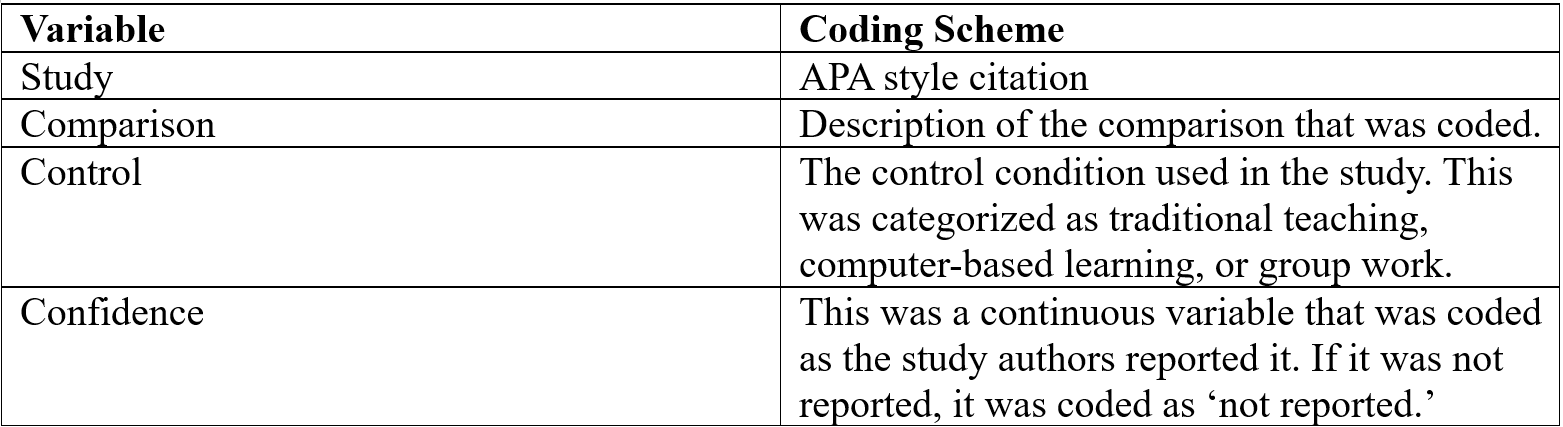
\includegraphics[width=1\textwidth,height=\textheight]{images/vartable.PNG}

\hypertarget{systematic-review-outcome-data-extraction}{%
\section{Systematic Review Outcome Data Extraction}\label{systematic-review-outcome-data-extraction}}

It is very difficult to provide guidance on how to set up your coding form for systematic reviews, simply because there are \emph{so} many different options. For example, do you want to know the fine-grained results, such as mean, standard deviations, and sample sizes? Or do you want to just know overall statistical test results? Or, maybe you only care about the conclusion the authors made based on those findings?

Regardless, you'll probably have key features you want to code from the studies. Depending on your research questions, these can vary widely. For example, you might be interested in publication trends, coding the year and type of publication. Or, you might be interested in the design of an intervention, coding features of the implementation. Or, you might be interested in the type of assessment used and code their qualities. Or, you might code all of these things. It really depends on your research questions. \ul{Your research questions should guide the data you extract from studies.}

\hypertarget{meta-analysis-outcome-data-extraction}{%
\section{Meta-Analysis Outcome Data Extraction}\label{meta-analysis-outcome-data-extraction}}

Metafor\citep{viechtbauer2010} uses two pieces of information for conducting the meta-analysis that you need to consider during your coding process: the effect size (\textbf{\emph{yi}}) and the variance (\textbf{\emph{vi}}). As such, you have choices when coding: you can code the mean, standard deviation, and sample size for the experimental and control groups and then use R and metafor to calculate the effect size and variance for each comparison (my recommended method), or you can calculate the effect size and variance for each effect size yourself. I prefer the former approach because I find it helpful to have all of this data to check for errors in coding (such as a misplaced decimal point -- these things happen!) and also for calculating sample sizes for tables.

If you choose to use R and metafor to calculate the effect sizes and variance, it will be important to have each mean, standard deviation, and sample size for the experimental group and the control group in their own columns (i.e., you'll need six columns to record this data). \textbf{The analysis codes in this book will assume this is the case.} I recommend having simple column titles that are descriptive, don't contain spaces, and are easy to remember, because you will have to type them into R.

Another important note I would like to make, because I see it so poorly reported in papers sometimes, is that \ul{you should be very purposeful in your selection of comparison groups}. Personally, I recommend that if given a choice (e.g., multiple control and/or experimental groups), you select the comparisons with the \textbf{fewest confounding variables.} Why? So you have more confidence that the effects you find are actually speaking to the intervention you're investigating rather than extraneous factors. If given a choice, I generally choose to ignore (that's right, I ignore data!) groups that present confounding variables when a non-confounded comparison is available. While that `leaves data on the table' so to speak, it makes for a more trustworthy analysis (in my opinion). One key thing to remember with meta-analysis is that if you use junk data, you'll get a junk result. So more data isn't necessarily better than ``cleaner'' (less confounded) data.

\hypertarget{conventional-meta-analysis}{%
\subsection{Conventional Meta-analysis}\label{conventional-meta-analysis}}

One key assumption of conventional meta-analysis is that of \ul{statistical independence - each participant can only be counted once.} Let's say you have a study that has three dependent variables, all of which are of interest to you - guess what, in conventional meta-analysis, you have to pick one dependent variable (or calculate weighted means and pooled standard deviations, but I do not prefer this method for reasons discussed in the \protect\hyperlink{0}{conventional meta-analysis chapter}). \textbf{Due to this, each comparison will appear on one row on your coding form.}

Let's look at some examples of different scenarios. Please note that you can have as many moderator variables as you wish, and they can be continuous or categorical.

Our first example is a study with one experiment and three groups: a control group, a group using clickers, and a group using clickers with self-reflection prompts. For the purposes of our example, we'll ignore the clicker with self-reflection prompts group, because a) we only have one control group, so we can only have one comparison or we violate the principle of statistical independence, and b) I don't like to combine groups for reasons discussed in the \protect\hyperlink{crossmeta}{conventional meta-analysis chapter}. This means we'll compare the control group and the clicker group. We'll also code for two moderator variables, the type of control condition (categorical) and the student's confidence level using clickers (continuous). Our coding form may look like this:

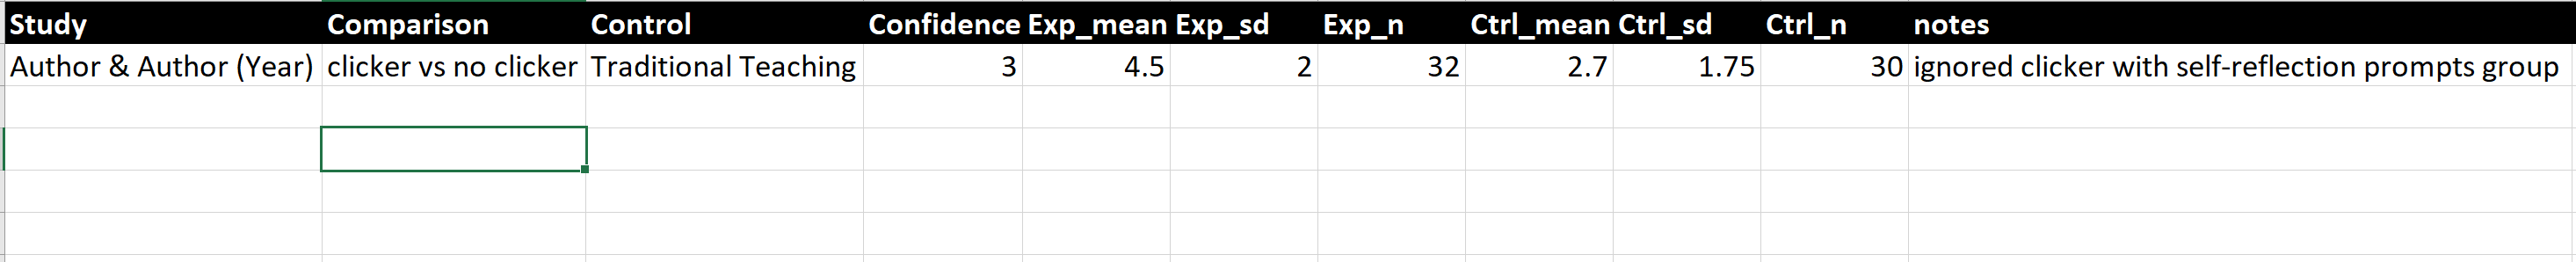
\includegraphics[width=2\textwidth,height=\textheight]{images/MA_coding.PNG}

\emph{What's this mean?}

Labels in the ``\textbf{Study}'' column will appear on the forest plots, so check your spelling and formatting unless you want to fix it later. (Unsolicited advice: nobody wants to fix something like this later, just type it in correctly the first time).

\textbf{Comparison} in this case is used so that I know what group's data I coded and so readers know what data I coded.

\textbf{Control} is a categorical moderator. I would have set choices for this before starting coding.

\textbf{Confidence} is a continuous variable.

\textbf{Exp\_mean} = mean of the experimental group

\textbf{Exp\_sd} = standard deviation of the experimental group

\textbf{Exp\_n} = sample size of the experimental group

\textbf{Ctrl\_mean} = mean of the control group

\textbf{Ctrl\_sd} = standard deviation of the control group

\textbf{Ctrl\_n} = sample size of the control group

\textbf{Notes} = my own notes on the paper

What if we have a study that has a design where there are two control groups (for our purposes) and two experimental groups? Well, luckily we can include all of them. Here's what that might look like if participants were split between low confidence and high confidence participants:

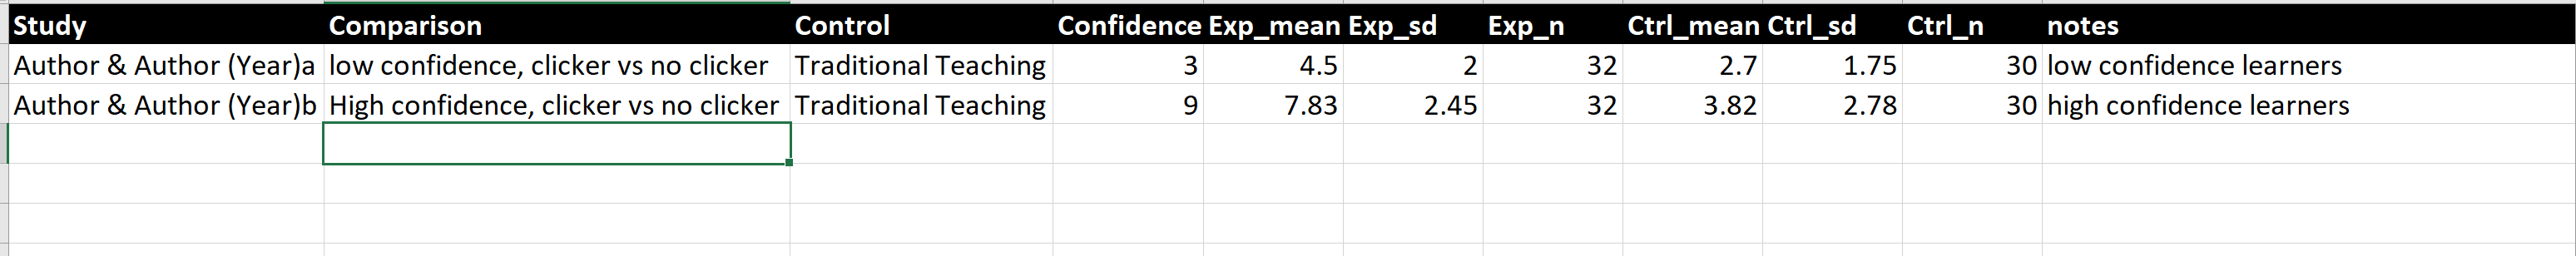
\includegraphics[width=2\textwidth,height=\textheight]{images/meta2.PNG}

\emph{What's this mean?}

Here you can see a few differences compared to the first example. Namely, in the study column I have separated the study names by adding an \textbf{`a'} and \textbf{`b'} to indicate that they are different comparisons in the same study.

Next, under ``\textbf{comparison}'' I indicated that one group was designated as the low confidence participants, and one was high confidence. Importantly - these are different participant groups with no overlap.

That's basically it. The most important thing to remember when coding a conventional meta-analysis is that \ul{\textbf{each participant can only be counted once.}}

\hypertarget{three-level-meta-analysis}{%
\subsection{Three-Level Meta-Analysis}\label{three-level-meta-analysis}}

As explained in the \protect\hyperlink{cross3LMA}{three-level meta-analysis chapter}, three-level meta-analysis can account for dependencies in the data. So, remember that study with three dependent variables that were important? Well, if we use three-level meta-analysis we can include all of that data!

There are some important things we should note about how to structure your coding form. These are best seen through an example, so let's analyze an example coding form. Note that just like conventional meta-analysis, you can have as many moderator variables as you wish, and they can be continuous or categorical.

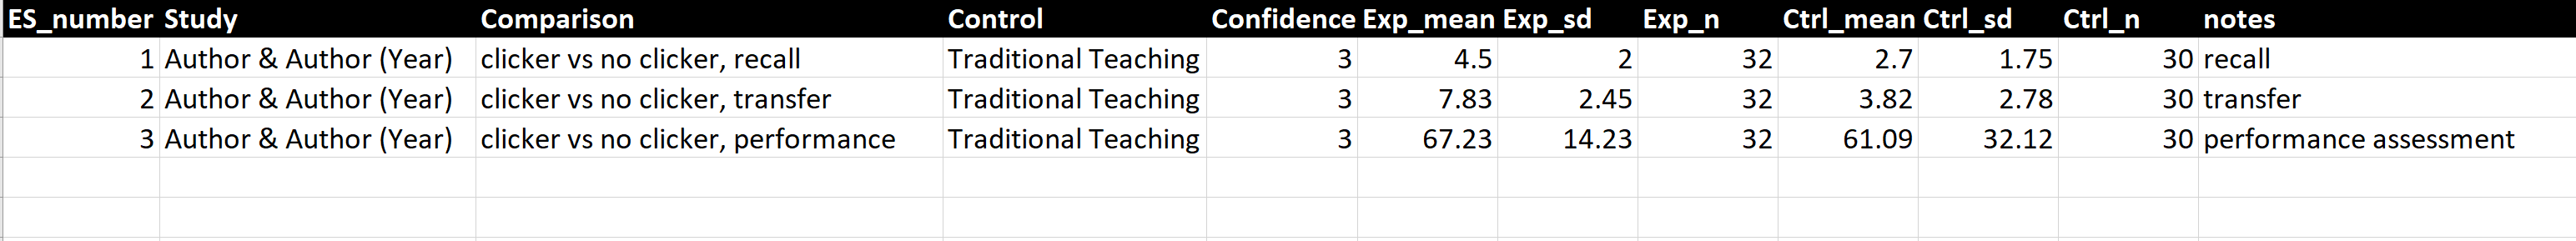
\includegraphics[width=2\textwidth,height=\textheight]{images/3lmacoding.PNG}

\emph{What's this mean?}

\textbf{ES\_number}: This column is unique to three-level meta-analysis. It should sequentially number every comparison in your coding form. There should not be duplicates.

\textbf{Study}: Similar to conventional meta-analysis, this should be the citation information as you want it to appear in your forest plot. However, \ul{unlike conventional meta-analysis, here you want the study name to be identical across all comparisons (rows) of data from this study}.

\textbf{Comparison}: Similar to conventional meta-analysis, this tells us what information we specifically examined. I indicated what type of outcome test this was from (i.e., recall, transfer, performance).

\textbf{Control}: This is a categorical moderator with pre-set categories.

\textbf{Confidence}: This is a continuous moderator. Note that it is the same for all comparisons because \ul{these are the same participants across all three rows.} This would be a huge violation of statistical independence in conventional meta-analysis, but that's why we're using three-level meta-analysis!

The rest of the columns are the same as in the conventional meta-analysis example.

\hypertarget{inter-rater-reliability-or-agreement-1}{%
\section{Inter-rater Reliability or Agreement}\label{inter-rater-reliability-or-agreement-1}}

You need to calculate inter-rater agreement or inter-rater reliability anytime you have more than one coder involved in the data extraction process. Even if you have one person coding the data, you should still have a second coder independently code a subset of the studies. Why? So you can find out a) if your first rater was accurate, b) if your coding scheme makes sense to another person, and c) to ensure your coding scheme is reliable. Generally speaking, I see 10-20\% of the sample dual coded for inter-rater agreement or reliability purposes. 20\% is what I would call ``standard'', while smaller percentages are occasionally used with larger reviews.

How do you calculate this? Well, it depends on what you are calculating. Many times I see a simple inter-rater agreement statistic reported as a percentage. This is OK. Cohen's kappa is another option if there are two raters. I've also seen correlation coefficients reported. What is most appropriate depends on your study and your data.

\hypertarget{summary-1}{%
\section{Summary}\label{summary-1}}

The single most important consideration in your coding when coding for a meta-analysis is the selection of comparisons. You do not want to violate the principle of statistical independence in conventional meta-analysis, and you don't want to introduce confounding variables in any type of meta-analysis.

\hypertarget{systematic-review-data-analysis}{%
\chapter{Systematic Review Data Analysis}\label{systematic-review-data-analysis}}

This chapter is going to be really short. Why? Well, because to analyze systematic review data, we're typically looking for themes in our data. To be honest, I don't have much more to say than that. However, there are a couple things I recommend:

\begin{itemize}
\item
  When I start analyzing my data, I make a spreadsheet for each research question, and move only the relevant data there. Be sure to keep your master coding form intact though!
\item
  Looking for patterns can be difficult. Remember that many spreadsheet programs have sorting features that may help you identify surface-level patterns.
\item
  Cross-tabulation can be a great way to look for interesting interactions between data points.
\end{itemize}

And that's really all I have to say about it. You're really looking for patterns in relation to each research question. If you need more guidance than that, I suggest reviewing some of the wonderful resources that have been written about analyzing qualitative data with, for example, content analysis or thematic analysis. They may be helpful for getting started if you feel overwhelmed by your data.

\hypertarget{part-meta-analysis-in-r}{%
\part{Meta-Analysis in R}\label{part-meta-analysis-in-r}}

\hypertarget{rbasics}{%
\chapter{R Basics}\label{rbasics}}

Alright, we're getting to the good stuff here, how to use R. You might be a bit anxious because R requires coding, but don't worry, we'll walk through everything step by step.

\hypertarget{why-use-r-when-a-gui-based-platform-is-easier}{%
\section{Why use R when a GUI-based Platform is Easier?}\label{why-use-r-when-a-gui-based-platform-is-easier}}

At the time of writing, GUI-based platforms such as \href{https://meta-analysis.com/}{Comprehensive Meta-Analysis} (paid software at the time of writing), \href{https://jasp-stats.org/}{JASP} (free software at the time of writing), and \href{https://www.jamovi.org/}{Jamovi} (free software at the time of writing) are excellent for conducting conventional meta-analyses. They can help you analyze the data quickly, without having to know how to do any coding in R. However, some of these options are limited in terms of reproducibility, meaning someone would need the same program to confirm your analysis. While this may seem like a minor limitation to some, it is actually quite important.

Another limitation of many GUI-based platform is that (at the time of writing) they do not allow one to conduct multivariate or three-level meta-analyses, among other limitations. In the educational sciences, three-level meta-analysis seems to offer advantages because you can account for, for example, all of the learning outcome tests in a study rather than only one learning outcome test per study. In other words, the three-level meta-analysis can account for the dependence between effect sizes, whereas a conventional (two-level) meta-analysis cannot. This factor alone is what convinced me that I needed to learn R!

One final thing I found I enjoyed about learning R and metafor\citep{viechtbauer2010} was that it taught me just how much you may not realize might be happening behind the scenes in GUI-based software. For example, do you know what estimator you're using in the GUI-based software? Are you using a Knapp-Hartung adjustment? These kinds of questions are important, yet you may not think about them if you just copy-pasted your data and asked the software to run the analysis.

\hypertarget{install-r-and-r-studio}{%
\section{Install R and R Studio}\label{install-r-and-r-studio}}

You can \href{https://www.r-project.org/}{download and install R here} and I recommend \href{https://posit.co/download/rstudio-desktop/}{downloading and installing R Studio} (free version) as well.

Once you have R and R Studio installed, you'll want to open R Studio.

\hypertarget{what-you-need-to-know}{%
\section{What You Need to Know}\label{what-you-need-to-know}}

What do I think you \emph{need} to know about R and R Studio before continuing in this book? Well, honestly not a lot. I've tried to break it down into very simple terms. I would install R and R Studio, then continue with the book as long as you know where to enter code into the file you're working on (top left of R Studio for me), where the console is (bottom left of R Studio for me), where the environment is (top right of R Studio for me), and where the files and plots appear (bottom right of R Studio for me), I think you'll likely be OK to move forward. Here's a screenshot of R Studio so you can see where everything is on my set up (which I believe is the default).

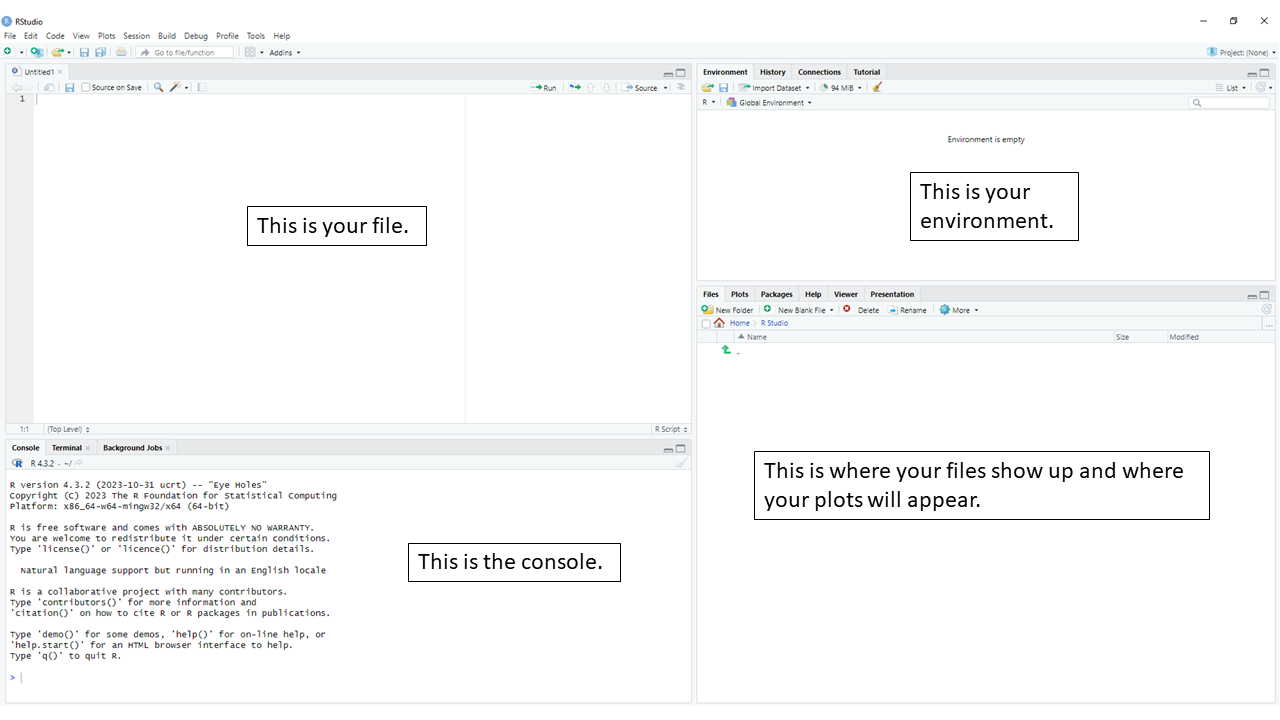
\includegraphics[width=1\textwidth,height=\textheight]{images/Rstudio.png}

\hypertarget{set-your-working-directory}{%
\subsection{Set Your Working Directory}\label{set-your-working-directory}}

You'll need to tell R where to save your files and where to retrieve files from, which is known as your working directory. There is not really a ``right'' or ``wrong'' way to do this. For simplicity, I set up a new project folder on my desktop, and I save my data file there. Then I set that folder as my working directory. To set your working directory, you click on session, then set working directory, as seen in the screenshot below. I would choose the ``choose directory'' option, then choose my desktop folder that is my project folder.

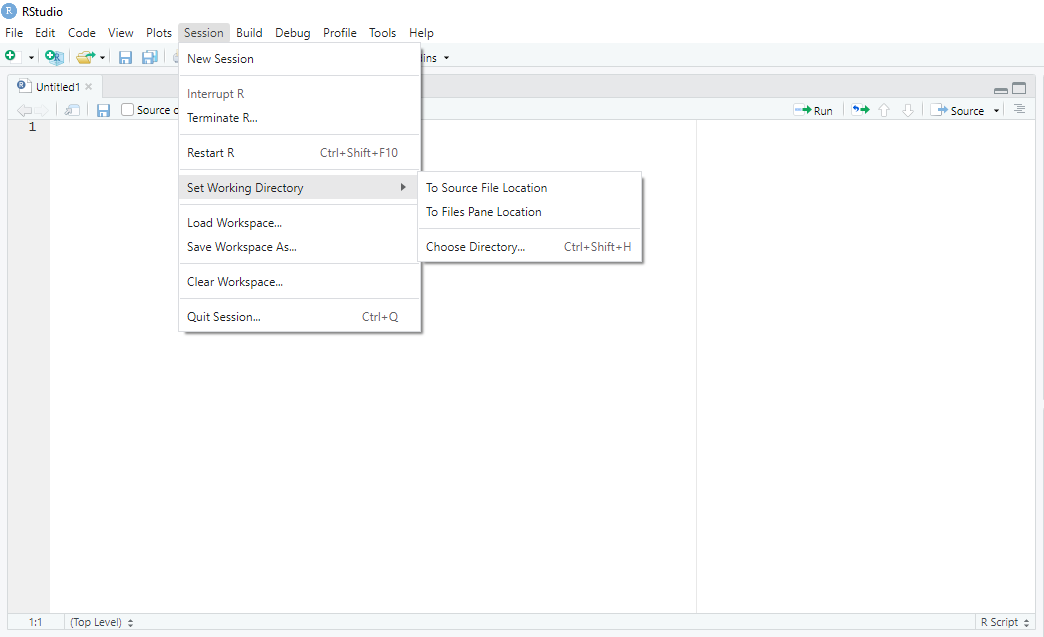
\includegraphics[width=1\textwidth,height=\textheight]{images/workingdirectory.PNG}

\hypertarget{install-r-packages-well-need-for-meta-analysis}{%
\subsection{Install R Packages We'll Need for Meta-Analysis}\label{install-r-packages-well-need-for-meta-analysis}}

We'll need to install a few R packages before continuing into this book. Fortunately, this is super easy! Let's see how to do this.

In your file (see screenshot above) you want to enter the following code:

\begin{Shaded}
\begin{Highlighting}[]
\CommentTok{\#install packages}
\FunctionTok{install.packages}\NormalTok{(}\StringTok{"metafor"}\NormalTok{)}
\FunctionTok{install.packages}\NormalTok{(}\StringTok{"tidyverse"}\NormalTok{)}
\FunctionTok{install.packages}\NormalTok{(}\StringTok{"plyr"}\NormalTok{)}
\FunctionTok{install.packages}\NormalTok{(}\StringTok{"grid"}\NormalTok{)}
\FunctionTok{install.packages}\NormalTok{(}\StringTok{"gridExtra"}\NormalTok{)}
\FunctionTok{install.packages}\NormalTok{(}\StringTok{"metaSEM"}\NormalTok{)}
\FunctionTok{install.packages}\NormalTok{(}\StringTok{"ggrepel"}\NormalTok{)}
\end{Highlighting}
\end{Shaded}

\emph{What will this code do?}

This code will install the named packages into your computer so that R understands the functions built into each one.

\emph{How do I get it to actually install or run code?}

Now that you've copy-pasted the code into your file, you want to highlight the code, then click `run' in the top right of the file area. See the screenshot below, where run is highlighted in red.

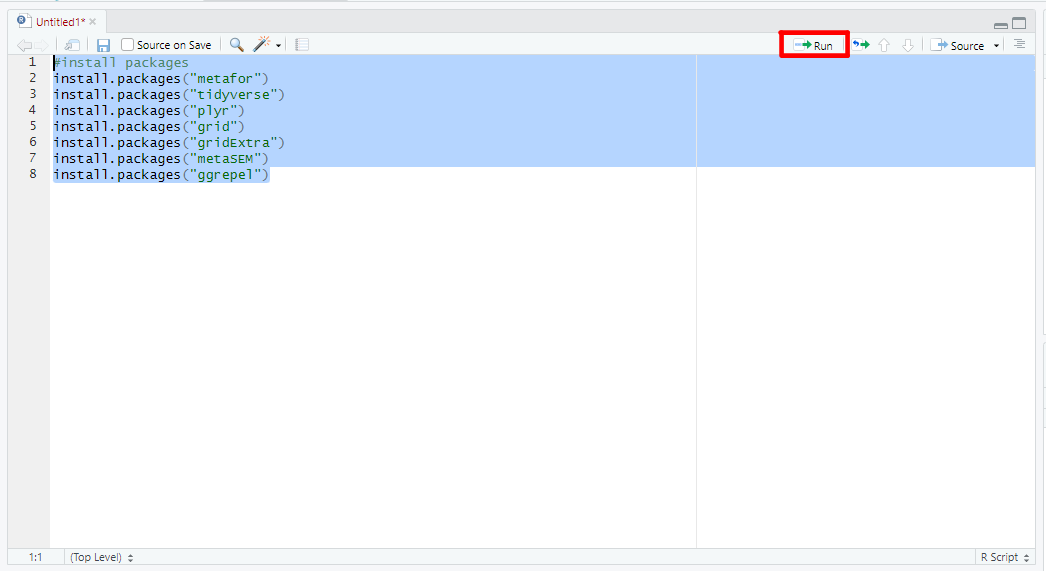
\includegraphics[width=1\textwidth,height=\textheight]{images/runbutton.PNG}

After you click run, you'll see things appear in the console. That's normal. It will take a few minutes for the packages to install, but once they're done, you're ready to move forward. Once a package is installed, you don't need to install it every time you run an analysis. We will just open them. If you don't know how to do that, don't worry, I'll walk you through this as we go through each chapter.

\hypertarget{was-that-easy}{%
\subsubsection{Was that easy?}\label{was-that-easy}}

If this first step was easy or you figured it out without too much trouble, I think you're ready to move forward in the book.

\hypertarget{was-this-too-difficult}{%
\subsubsection{Was this too difficult?}\label{was-this-too-difficult}}

If you struggled to keep up so far, then I would suggest you start at the very basics. There are so many resources online, I don't see a reason to rewrite what others have written about extensively. I know getting started with R Studio can be intimidating. It seems scary and complicated. After you get started and start writing your own code, it won't seem so scary. Here is a starting point: \url{https://education.rstudio.com/learn/beginner/}

\hypertarget{meta}{%
\chapter{Conventional Meta-Analysis}\label{meta}}

This chapter will cover the basics of conventional (two-level) meta-analysis in R using metafor \citep{viechtbauer2010}. In conventional meta-analysis, a very important limitation is known as the \textbf{principle of statistical independence}, meaning that each participant can only be counted once. What does this mean for you as a researcher?

Let's look at an example: Say you are comparing the impact of a computer on learners' reading proficiency compared to other media. You found a study that meets your inclusion criteria but it has three groups: a computer group, a tablet group, and a paper book group. You can see you have two possible comparisons here: computer vs tablet, and computer vs paper book. You may think that you can include both of these comparisons in your conventional meta-analysis. \textbf{However, this is incorrect.} Doing this would count the computer group twice, therefore violating the principle of statistical independence. As such, \ul{you must make a decision}: which comparison do you want to include? Alternatively, you could (but I wouldn't) take the weighted mean and pooled standard deviation of the two non-computer groups to create a comparison that does not duplicate the computer group's scores. I say I would not do this latter approach because it will add conflating factors into your analysis. Remember - a meta-analysis is only as useful as the types of data that went into it!

Another popular issue is the question of fixed effects and random effects models. Simply stated, we almost always use random effects models in education, so all examples in this book will use random effects. If you don't know the differences between fixed and random effects meta-analysis models, please see \citep{borenstein2010}.

If you aren't familiar with conventional meta-analysis, please read about it before conducting one. There are plenty of free resources available. I would recommend starting with the great, free book, \href{https://bookdown.org/MathiasHarrer/Doing_Meta_Analysis_in_R/}{Doing Meta-Analysis in R}\citep{harrer2021}.

Let's say you understand the differences between conventional and three-level meta-analytic models, you understand what meta-analysis is used for, and you've decided you're moving ahead with the conventional model. Let's explore how to do this in R with metafor\citep{viechtbauer2010} using standardized mean differences as the effect size.

\hypertarget{preparing-your-data}{%
\section{Preparing your data}\label{preparing-your-data}}

Hopefully you have already run your \protect\hyperlink{crossliteraturesearch}{literature search}, \protect\hyperlink{crossscreening}{screened your studies}, and \protect\hyperlink{crossdata}{extracted your data}. This point forward assumes you have already completed these steps.

\hypertarget{your-data-file}{%
\subsection{Your Data File}\label{your-data-file}}

Personally I prefer to use .csv files as my data file that I import into R. Why? Because that's what was always used in the examples I found online when I was learning R, and I've used it ever since. Why change something that works? Plus, .csv works with many different software programs and across various operating systems. ~

As noted in the \protect\hyperlink{crossdata}{data extraction and coding chapter}, metafor uses two pieces of information for conducting the meta-analysis that you need to consider before importing data in R: the effect size (\textbf{\emph{yi}}) and the variance (\textbf{\emph{vi}}). If you read the previous chapters, you know you have choices when coding: you can code the mean, standard deviation, and sample size for the experimental and control groups and then use R and metafor to calculate the effect size and variance for each comparison (my recommended method), or you can calculate the effect size and variance for each effect size yourself. I prefer the former approach because I find it helpful to have all of this data to not only check for errors in coding (such as a misplaced decimal point -- these things happen!) and also for calculating sample sizes for tables.

If you choose to use R and metafor to calculate the effect sizes and variance, it will be important to have each mean, standard deviation, and sample size for the experimental group and the control group in their own columns. I recommend having simple column titles that are descriptive and easy to remember, because you will have to type them into R. \textbf{See a sample coding form below, which we will use for our conventional meta-analysis}. Note that you can have as many moderator variables as you wish, and they can be continuous or categorical.

So, assuming you have all of that done, let's get onto the fun stuff, running a conventional meta-analysis!

\hypertarget{running-a-conventional-meta-analysis-with-metafor}{%
\section{Running a Conventional Meta-Analysis with Metafor}\label{running-a-conventional-meta-analysis-with-metafor}}

\hypertarget{example-data-for-this-analysis}{%
\subsection{Example Data for This Analysis}\label{example-data-for-this-analysis}}

If you want to follow along with this specific example, you'll want to use the subset of data from Schroeder and Cenkci's (2018)\citep{schroeder2018} meta-analysis on the spatial split-attention effect. The data can be downloaded here.

\hypertarget{load-r-packages}{%
\subsection{Load R Packages}\label{load-r-packages}}

First we need to load our R packages. Hopefully you installed these already, if not it won't take long, just see the \protect\hyperlink{crossrpackages}{R Basics chapter}. Assuming you have already installed the R packages, let's load them up so we can do some meta-analysis!

\begin{Shaded}
\begin{Highlighting}[]
\CommentTok{\#load metafor}
\FunctionTok{library}\NormalTok{(metafor)}
\FunctionTok{library}\NormalTok{(tidyverse)}
\end{Highlighting}
\end{Shaded}

\emph{What's this code doing?}

This code is simply loading the metafor package in the R environment so we can do our analysis. It's also loading tidyverse, which we'll use to help us calculate participant numbers and create tables.

\hypertarget{import-your-data-into-r-studio}{%
\subsection{Import Your Data Into R Studio}\label{import-your-data-into-r-studio}}

The first step to conducting your meta-analysis is to read in the data. To do that, we first want to set our working directory (more about that in the \protect\hyperlink{crossrbasics}{R Basics chapter}). Once you've set your working directory, you can use this piece of code.

\begin{Shaded}
\begin{Highlighting}[]
\CommentTok{\#name data file and read in .csv. }
\NormalTok{dat }\OtherTok{\textless{}{-}} \FunctionTok{read.csv}\NormalTok{(}\StringTok{"SC sample data.csv"}\NormalTok{)}
\end{Highlighting}
\end{Shaded}

\emph{What's this code doing?\\
}You see the first piece of code is `\textbf{dat}', which is what we are going to name our data file. The \textbf{\textless-} indicates that you are going to name something. The next piece is telling R to read in a .csv file from the working directory, and then you can see the file name I used. So basically, we're saying \emph{import this data from a .csv file and call it dat.}

After you run this, you'll see an item called `dat' appear in your environment, which contains your data!

\hypertarget{calculating-effect-sizes}{%
\subsection{Calculating Effect Sizes}\label{calculating-effect-sizes}}

Next, you will want to calculate the effect sizes and variance for each effect size if you have not done so already. You can do that using this code:

\begin{Shaded}
\begin{Highlighting}[]
\CommentTok{\#calculate overall ES, in this case standardized mean difference (Hedges g), and variance.}

\NormalTok{dat1 }\OtherTok{\textless{}{-}} \FunctionTok{escalc}\NormalTok{(}\AttributeTok{measure=}\StringTok{"SMD"}\NormalTok{, }\AttributeTok{m1i=}\NormalTok{Exp\_mean, }\AttributeTok{sd1i=}\NormalTok{Exp\_sd, }\AttributeTok{n1i=}\NormalTok{Exp\_n, }\AttributeTok{m2i=}\NormalTok{Ctrl\_mean, }\AttributeTok{sd2i=}\NormalTok{Ctrl\_sd, }\AttributeTok{n2i=}\NormalTok{Ctrl\_n, }\AttributeTok{data=}\NormalTok{dat)}
\end{Highlighting}
\end{Shaded}

\emph{What's this code doing?}

\textbf{dat1 \textless-} indicates naming a new datafile.

In this case you're doing a calculation, \textbf{Escalc} is telling it calculate an effect size. Within that function, \textbf{measure=``SMD''} is saying we want to use the standardized mean difference.

The next set of variables (\textbf{m1i, sd1i, n1i, m2i, sd2i,} and \textbf{n2i}) are specific pieces of information that metafor needs to calculate the effect size. \textbf{m1i} is the mean of the intervention group. \textbf{sd1i} is the standard deviation of the intervention group. \textbf{n1i} is the sample size of the intervention group. \textbf{m2i} is the mean of the control group. \textbf{sd2i} is the standard deviation of the control group. \textbf{n2i} is the sample size of the control group. I have always found those codes hard to remember, so on my coding form/data file I use different column headings. You can see I tell metafor where to find each variable by using the \textbf{=} sign. For example, the mean of the intervention group (\textbf{m1i}) is called \textbf{Exp\_mean} in my data file.

Finally, we need to tell metafor where to find the data, and we have to refer to data already in R. We use our datafile `\textbf{dat}'.

Now if you can make sure the effect size and variance for each effect size were calculated:

\begin{Shaded}
\begin{Highlighting}[]
\CommentTok{\#display data}
\NormalTok{dat1}
\end{Highlighting}
\end{Shaded}

\emph{What's this code doing?}

This will display your full data set saved as `\textbf{dat1}' in the console.

However, I find this kind of hard to read if I have a lot of data. So, I prefer to write it all to a .csv file instead because I find it easier to read. This code can do that:

\begin{Shaded}
\begin{Highlighting}[]
\CommentTok{\#save .csv file with ES data. This goes into working directory}
\FunctionTok{write.csv}\NormalTok{(dat1, }\AttributeTok{file =} \StringTok{"ESdata.csv"}\NormalTok{)}
\end{Highlighting}
\end{Shaded}

\emph{What's this code doing?}

The \textbf{write.csv} tells R you want to create a .csv file. This will be saved in your working directory.

The \textbf{dat1} is telling R which data you want to write into the .csv file.

\textbf{file = ``ESdata.csv''} is simply naming the datafile whatever you have between the '' ``. You can name it whatever you want, but my example will use ESdata as the file name, and I'll assume this is the case through the rest of the analysis.

You're probably wondering, \emph{Why write a .csv file with the effect size and variance data when it is saved in R?}

Well, I like to look at the .csv file and make sure I don't see any effect sizes that seem very wrong. If I find any then it is easy for me to track back to which study it came from and I can see if I made a mistake during coding. A misplaced decimal point can have huge implications for your analysis - this is a step that helps you catch those human errors.

\hypertarget{running-the-meta-analysis-model}{%
\section{Running The Meta-Analysis Model}\label{running-the-meta-analysis-model}}

Now the part we've all been waiting for, let's run a meta-analysis model! We can use this code:

\begin{Shaded}
\begin{Highlighting}[]
\CommentTok{\#run overall random effects meta{-}analysis}
\NormalTok{overallresult }\OtherTok{\textless{}{-}} \FunctionTok{rma}\NormalTok{(yi, vi, }\AttributeTok{data=}\NormalTok{dat1)}
\end{Highlighting}
\end{Shaded}

\emph{What's this code doing?}

First, we're naming our meta-analysis result as a new piece of data in R, and we're naming it `\textbf{overallresult}'

\textbf{rma} is telling metafor that we want to run a random-effects, conventional meta-analysis model. Within that, we're using \textbf{yi} to reference effect size data within our data set (this is a column heading), \textbf{vi} to reference effect size variance within our data set (this is a column heading), and \textbf{data = dat1} is simply telling metafor which data set within R to reference when running the analysis. Note that we're using dat1, rather than dat, because dat1 contains the effect sizes and variances we calculated, whereas dat does not.

So we ran this code and\ldots. seemingly nothing happened? Well, if you look at your environment, you'll see the new item called overall result. Let's view that in our console now so we can see the overall result of our meta-analysis:

\begin{Shaded}
\begin{Highlighting}[]
\CommentTok{\#display meta{-}analysis result}
\NormalTok{overallresult}
\end{Highlighting}
\end{Shaded}

\emph{What's this code doing?}

This code simply displays the result in the console so you can see the meta-analysis result.

\hypertarget{interpreting-the-results}{%
\subsection{Interpreting the Results}\label{interpreting-the-results}}

When we run that code, we now see the following:

\begin{verbatim}
Random-Effects Model (k = 27; tau^2 estimator: REML)

tau^2 (estimated amount of total heterogeneity): 0.2372 (SE = 0.0940)
tau (square root of estimated tau^2 value):      0.4870
I^2 (total heterogeneity / total variability):   73.51%
H^2 (total variability / sampling variability):  3.77

Test for Heterogeneity:
Q(df = 26) = 90.0975, p-val < .0001

Model Results:

estimate      se    zval    pval   ci.lb   ci.ub      
  0.6142  0.1127  5.4512  <.0001  0.3934  0.8351  *** 

---
Signif. codes:  0 ‘***’ 0.001 ‘**’ 0.01 ‘*’ .05 ‘.’ 0.1 ‘ ’ 1
\end{verbatim}

\emph{What's this mean?}

Recall this is a subset of data from Schroeder and Cenkci (2018)\citep{schroeder2018}, so the numbers will not align with what is in the published version.

The first line tells us this is a random-effects model including 27 comparisons, and tau\textsuperscript{2} was estimated using restricted maximum likelihood estimation (REML).

Typically, the important pieces here that we are interested in reporting in our manuscript are the overall effect size, the \emph{Q}-test, and the \emph{I}\textsuperscript{2}.

The effect size (the estimate under the model results) is interpreted as the standardized mean difference effect size, if there is a significant \emph{Q} test it indicates there is significant heterogeneity in our sample, and the \emph{I}\textsuperscript{2} statistic gives us a percentage that is commonly used to report between-study heterogeneity.

\hypertarget{checking-for-outliers-and-influence}{%
\subsection{Checking for Outliers and Influence}\label{checking-for-outliers-and-influence}}

At this point we've ran our random-effects meta-analysis model. However, we have not checked for outliers or studies with significant influence on the results. This is actually a complex topic, as not many meta-analyses (as of January, 2024) in education actually address a) if they searched for outliers or influence, b) what metric they used to check for outliers and why, and c) what they did about the outliers and why. Kinda of interesting right?

So here's what we can do to check for outliers and influence. We'll follow Viechtbauer and Cheung's (2010) \citep{viechtbauer2010a} process, which fortunately is built right into metafor. Similarly, you should also know about \href{https://wviechtb.github.io/metafor/reference/influence.rma.uni.html}{this website} which describes the function we'll use.

\begin{Shaded}
\begin{Highlighting}[]
\CommentTok{\#check for outliers}
\FunctionTok{influence}\NormalTok{(overallresult)}
\end{Highlighting}
\end{Shaded}

\emph{What's this code doing?}

This tells metafor to produce influence diagnostics for the meta-analysis model (which we called `\textbf{overallresult}' in an earlier step).

Once we run that, we'll see a bunch of data in the console. It'll look like this:

\begin{Shaded}
\begin{Highlighting}[]
\NormalTok{  rstudent  dffits cook.d  cov.r tau2.del  QE.del    hat weight    dfbs inf }
\DecValTok{1}    \FloatTok{0.6685}  \FloatTok{0.1352} \FloatTok{0.0188} \FloatTok{1.0679}   \FloatTok{0.2458} \FloatTok{87.9029} \FloatTok{0.0394} \FloatTok{3.9410}  \FloatTok{0.1353}     
\DecValTok{2}    \FloatTok{0.9087}  \FloatTok{0.1928} \FloatTok{0.0375} \FloatTok{1.0537}   \FloatTok{0.2399} \FloatTok{84.8441} \FloatTok{0.0432} \FloatTok{4.3182}  \FloatTok{0.1929}     
\DecValTok{3}    \FloatTok{0.5790}  \FloatTok{0.1083} \FloatTok{0.0120} \FloatTok{1.0629}   \FloatTok{0.2462} \FloatTok{88.9252} \FloatTok{0.0336} \FloatTok{3.3650}  \FloatTok{0.1081}     
\DecValTok{4}   \SpecialCharTok{{-}}\FloatTok{1.5995} \SpecialCharTok{{-}}\FloatTok{0.3258} \FloatTok{0.0986} \FloatTok{0.9709}   \FloatTok{0.2146} \FloatTok{81.8692} \FloatTok{0.0397} \FloatTok{3.9747} \SpecialCharTok{{-}}\FloatTok{0.3253}     
\DecValTok{5}   \SpecialCharTok{{-}}\FloatTok{0.5008} \SpecialCharTok{{-}}\FloatTok{0.1096} \FloatTok{0.0126} \FloatTok{1.0913}   \FloatTok{0.2509} \FloatTok{88.7138} \FloatTok{0.0464} \FloatTok{4.6375} \SpecialCharTok{{-}}\FloatTok{0.1100}     
\DecValTok{6}   \SpecialCharTok{{-}}\FloatTok{0.5864} \SpecialCharTok{{-}}\FloatTok{0.1030} \FloatTok{0.0108} \FloatTok{1.0550}   \FloatTok{0.2451} \FloatTok{89.5042} \FloatTok{0.0296} \FloatTok{2.9570} \SpecialCharTok{{-}}\FloatTok{0.1027}     
\DecValTok{7}   \SpecialCharTok{{-}}\FloatTok{0.9935} \SpecialCharTok{{-}}\FloatTok{0.2231} \FloatTok{0.0498} \FloatTok{1.0501}   \FloatTok{0.2371} \FloatTok{81.6753} \FloatTok{0.0480} \FloatTok{4.8003} \SpecialCharTok{{-}}\FloatTok{0.2231}     
\DecValTok{8}    \FloatTok{1.3164}  \FloatTok{0.2661} \FloatTok{0.0684} \FloatTok{1.0066}   \FloatTok{0.2262} \FloatTok{83.0741} \FloatTok{0.0391} \FloatTok{3.9107}  \FloatTok{0.2659}     
\DecValTok{9}    \FloatTok{3.7924}  \FloatTok{0.6914} \FloatTok{0.3325} \FloatTok{0.6777}   \FloatTok{0.1237} \FloatTok{61.5550} \FloatTok{0.0340} \FloatTok{3.4049}  \FloatTok{0.7120}   \SpecialCharTok{*} 
\DecValTok{10}  \SpecialCharTok{{-}}\FloatTok{0.2785} \SpecialCharTok{{-}}\FloatTok{0.0576} \FloatTok{0.0035} \FloatTok{1.0906}   \FloatTok{0.2525} \FloatTok{89.9252} \FloatTok{0.0412} \FloatTok{4.1216} \SpecialCharTok{{-}}\FloatTok{0.0577}     
\DecValTok{11}   \FloatTok{0.3018}  \FloatTok{0.0598} \FloatTok{0.0037} \FloatTok{1.0827}   \FloatTok{0.2511} \FloatTok{89.5783} \FloatTok{0.0379} \FloatTok{3.7881}  \FloatTok{0.0598}     
\DecValTok{12}   \FloatTok{0.2050}  \FloatTok{0.0421} \FloatTok{0.0019} \FloatTok{1.0918}   \FloatTok{0.2530} \FloatTok{89.7261} \FloatTok{0.0409} \FloatTok{4.0860}  \FloatTok{0.0421}     
\DecValTok{13}  \SpecialCharTok{{-}}\FloatTok{0.4720} \SpecialCharTok{{-}}\FloatTok{0.0961} \FloatTok{0.0096} \FloatTok{1.0802}   \FloatTok{0.2496} \FloatTok{89.4834} \FloatTok{0.0399} \FloatTok{3.9877} \SpecialCharTok{{-}}\FloatTok{0.0962}     
\DecValTok{14}  \SpecialCharTok{{-}}\FloatTok{1.0632} \SpecialCharTok{{-}}\FloatTok{0.2193} \FloatTok{0.0478} \FloatTok{1.0359}   \FloatTok{0.2351} \FloatTok{86.1101} \FloatTok{0.0408} \FloatTok{4.0790} \SpecialCharTok{{-}}\FloatTok{0.2193}     
\DecValTok{15}   \FloatTok{0.0796}  \FloatTok{0.0165} \FloatTok{0.0003} \FloatTok{1.0966}   \FloatTok{0.2541} \FloatTok{89.9615} \FloatTok{0.0422} \FloatTok{4.2171}  \FloatTok{0.0165}     
\DecValTok{16}   \FloatTok{0.0159}  \FloatTok{0.0028} \FloatTok{0.0000} \FloatTok{1.0733}   \FloatTok{0.2502} \FloatTok{90.0770} \FloatTok{0.0319} \FloatTok{3.1859}  \FloatTok{0.0028}     
\DecValTok{17}   \FloatTok{1.3506}  \FloatTok{0.2737} \FloatTok{0.0721} \FloatTok{1.0025}   \FloatTok{0.2249} \FloatTok{82.6657} \FloatTok{0.0393} \FloatTok{3.9277}  \FloatTok{0.2735}     
\DecValTok{18}   \FloatTok{0.5500}  \FloatTok{0.1096} \FloatTok{0.0124} \FloatTok{1.0730}   \FloatTok{0.2479} \FloatTok{88.6613} \FloatTok{0.0383} \FloatTok{3.8253}  \FloatTok{0.1096}     
\DecValTok{19}   \FloatTok{0.3245}  \FloatTok{0.0610} \FloatTok{0.0039} \FloatTok{1.0737}   \FloatTok{0.2496} \FloatTok{89.6452} \FloatTok{0.0340} \FloatTok{3.4041}  \FloatTok{0.0609}     
\DecValTok{20}   \FloatTok{0.4078}  \FloatTok{0.0775} \FloatTok{0.0062} \FloatTok{1.0724}   \FloatTok{0.2489} \FloatTok{89.4124} \FloatTok{0.0347} \FloatTok{3.4717}  \FloatTok{0.0773}     
\DecValTok{21}  \SpecialCharTok{{-}}\FloatTok{0.3888} \SpecialCharTok{{-}}\FloatTok{0.0719} \FloatTok{0.0053} \FloatTok{1.0689}   \FloatTok{0.2485} \FloatTok{89.8413} \FloatTok{0.0327} \FloatTok{3.2714} \SpecialCharTok{{-}}\FloatTok{0.0718}     
\DecValTok{22}  \SpecialCharTok{{-}}\FloatTok{0.6555} \SpecialCharTok{{-}}\FloatTok{0.1428} \FloatTok{0.0211} \FloatTok{1.0797}   \FloatTok{0.2474} \FloatTok{87.7178} \FloatTok{0.0458} \FloatTok{4.5805} \SpecialCharTok{{-}}\FloatTok{0.1433}     
\DecValTok{23}  \SpecialCharTok{{-}}\FloatTok{0.0092} \SpecialCharTok{{-}}\FloatTok{0.0020} \FloatTok{0.0000} \FloatTok{1.0920}   \FloatTok{0.2534} \FloatTok{90.0749} \FloatTok{0.0400} \FloatTok{3.9967} \SpecialCharTok{{-}}\FloatTok{0.0020}     
\DecValTok{24}  \SpecialCharTok{{-}}\FloatTok{1.5371} \SpecialCharTok{{-}}\FloatTok{0.2464} \FloatTok{0.0592} \FloatTok{0.9875}   \FloatTok{0.2247} \FloatTok{86.1028} \FloatTok{0.0257} \FloatTok{2.5745} \SpecialCharTok{{-}}\FloatTok{0.2480}     
\DecValTok{25}   \FloatTok{0.7452}  \FloatTok{0.1174} \FloatTok{0.0139} \FloatTok{1.0383}   \FloatTok{0.2416} \FloatTok{88.9126} \FloatTok{0.0240} \FloatTok{2.4018}  \FloatTok{0.1171}     
\DecValTok{26}  \SpecialCharTok{{-}}\FloatTok{1.6889} \SpecialCharTok{{-}}\FloatTok{0.2854} \FloatTok{0.0780} \FloatTok{0.9711}   \FloatTok{0.2184} \FloatTok{84.7843} \FloatTok{0.0287} \FloatTok{2.8680} \SpecialCharTok{{-}}\FloatTok{0.2875}     
\DecValTok{27}  \SpecialCharTok{{-}}\FloatTok{1.0243} \SpecialCharTok{{-}}\FloatTok{0.1771} \FloatTok{0.0313} \FloatTok{1.0289}   \FloatTok{0.2369} \FloatTok{88.1449} \FloatTok{0.0290} \FloatTok{2.9037} \SpecialCharTok{{-}}\FloatTok{0.1771}
\end{Highlighting}
\end{Shaded}

\emph{What's this result mean?}

While this data looks scary at first, it's actually really easy to interpret. Why? Well, check that last column labeled `inf'. This tells us if any studies were outliers or significantly influenced our results. From here we can see that study 9 was potentially an outlier or had a significant influence on the result. You can read about influence diagnostics and the metrics used \href{https://wviechtb.github.io/metafor/reference/influence.rma.uni.html}{here} and in Viechtbauer and Cheung (2010)\citep{viechtbauer2010b}.

We know from this data that study 9 in our dataset is a potential outlier or has significant influence on our result. What do we do from here? Well, there's a lot of options, but here are my recommended steps:

\begin{itemize}
\item
  Go back to your data and check the effect size. Is it oddly large or small? If so, check and see if you have a typo in the data.
\item
  Let's say the data has no errors. Next we'll look at the study itself. Is there something substantially methodologically `wrong' or is it significantly different than the other studies in your sample? If so, you may be able to rationalize removing the study from your data set. If you do remove it, be sure to report that you did, and why, in your manuscript.
\item
  Ok so now things get real: Let's say your data is good, and the study itself was pretty well-done and not notably different than your other studies in the sample. What do you do? Well, that's a matter of opinion.

  \begin{itemize}
  \item
    My personal opinion is generally to retain the study as is - because it is valid data.
  \item
    Another option is to ``downsize'' the effect size to slightly larger (or smaller) than the next largest (or smallest) effect size.

    \begin{itemize}
    \tightlist
    \item
      I don't prefer this approach because I think valid data should be examined as valid data, but this is a reasonable option. The problem I have with this approach is that I have never seen a metric for how much ``larger'' or ``smaller'' you should change the effect size to. So I guess you just\ldots{} guess? That seems imprecise to me and since it can/will influence your whole analysis, I don't like that.
    \end{itemize}
  \item
    A final option is to remove the outlier from the dataset.

    \begin{itemize}
    \tightlist
    \item
      I generally don't like this option because I cannot rationalize it if the study was consistent with the rest in the analysis.
    \end{itemize}
  \end{itemize}
\end{itemize}

For the purposes of this example, we'll assume that the data are good, and there was nothing particularly notable about the study itself. Therefore we will retain the effect size in the data.

\hypertarget{writing-up-the-results}{%
\subsection{Writing up the Results}\label{writing-up-the-results}}

So if we were going to write this up, we may report something like this:

\begin{quote}
We conducted a random-effects meta-analysis of 27 independent comparisons. Our results indicated that the intervention was significantly better than the control condition (\emph{g} = .61, \emph{p} \textless{} .001). Moreover, the model indicates that there is significantly heterogeneity within the sample (\emph{Q}(26) = 90.10, \emph{p} \textless{} .001), and 73.51\% of the variance within the sample is due to between-study heterogeneity. We detected one study as a potential outlier or as having significant influence on the overall effect size, however examination of the study did not indicate any notable deviations from other studies in our sample. As such, the study was retained in the data analysis.
\end{quote}

\hypertarget{forest-plots}{%
\subsection{Forest Plots}\label{forest-plots}}

We should always include a forest plot with our results. We can create one with this code:

\begin{Shaded}
\begin{Highlighting}[]
\CommentTok{\#forest plot run this entire code section together. }
\NormalTok{forestplotdetails}\OtherTok{\textless{}{-}}\FunctionTok{forest.rma}\NormalTok{(overallresult, }\AttributeTok{slab=}\FunctionTok{paste}\NormalTok{(dat1}\SpecialCharTok{$}\NormalTok{studyauthor), }\AttributeTok{main =} \StringTok{"Forest Plot of Observed Effects"}\NormalTok{, }\AttributeTok{header=}\StringTok{"Author(s) and Year"}\NormalTok{)}
\CommentTok{\#this sets the text labels. first text position is X axis, second is y. }
\NormalTok{op }\OtherTok{\textless{}{-}} \FunctionTok{par}\NormalTok{(}\AttributeTok{cex=}\NormalTok{.}\DecValTok{75}\NormalTok{, }\AttributeTok{font=}\DecValTok{2}\NormalTok{)}
\FunctionTok{text}\NormalTok{(}\SpecialCharTok{{-}}\FloatTok{7.75}\NormalTok{, }\DecValTok{60}\NormalTok{, }\StringTok{"Authors and Year"}\NormalTok{, }\AttributeTok{pos=}\DecValTok{4}\NormalTok{)}
\FunctionTok{text}\NormalTok{(}\DecValTok{10}\NormalTok{, }\DecValTok{60}\NormalTok{, }\StringTok{"Effect Size (g) [95\% CI]"}\NormalTok{, }\AttributeTok{pos=}\DecValTok{2}\NormalTok{)}
\FunctionTok{par}\NormalTok{(op)}
\NormalTok{forestplotdetails }\DocumentationTok{\#\#this will print details for forest plot size which helps with text location}
\end{Highlighting}
\end{Shaded}

\emph{What's this code doing?}

This code is more complex, but we can look at some bigger pieces of it. The first line is setting `\textbf{forestplotdetails}' as a named data in your R environment. Then you're referencing a function in metafor (\textbf{forest.rma}) and telling it to use the data from `\textbf{overallresult}', our meta-analysis result in the R environment. Next we see `\textbf{slab=paste\ldots.}' and this is telling metafor which dataset to use (\textbf{dat1}). The \textbf{\$studyauthor} tells metafor where to get the data to fill in the Author and Year column in our dataset. The `\textbf{main}' and `\textbf{header}' are for the headings on the forest plot.

The rest of the code is more complex and has to do with the specifics of setting the specific titles. I copy-pasted it from example code I found online and it has worked for me. You may find you need to move the text positions, which is why the \textbf{forestplotdetails} data might be helpful.

If this code works correctly for you, the forest plot should appear in the plots section of R studio. You can save it by clicking on export (in the toolbar above the plot), and following the options to save the file.

\hypertarget{moderator-analysis}{%
\subsection{Moderator Analysis}\label{moderator-analysis}}

We've ran our overall random-effects meta-analysis model. Some people think this is the important finding, but in education, I think this result is generally only \emph{kind of} interesting. The \emph{really} good stuff, in my opinion, is examining all the potential moderator variables. Essentially, we're going to check and see what variables may influence the overall effect size.

What might be a moderator variable? Well, it depends on your field and the intervention you're investigating. In educational technologies, we typically examine participant characteristics, study characteristics, and intervention characteristics as potential moderators.

So, let's get right to it! We're going to focus on categorical moderators because there are a plethora of resources online about how to run continuous moderators.

\textbf{WARNING}: To run a categorical moderator analysis in metafor is actually two steps and they look similar. Let's take a look at the different steps.

\hypertarget{calculate-qbetween}{%
\subsubsection{\texorpdfstring{Calculate Q\textsubscript{between}}{Calculate Qbetween}}\label{calculate-qbetween}}

First we need to calculate Q\textsubscript{between}. This is an omnibus test that will tell us if there are significant differences \ul{between levels of the moderator}. We're going to use grade range as our example:

\begin{Shaded}
\begin{Highlighting}[]
\CommentTok{\#moderator test to calculate qbetween value. }
\NormalTok{mod.gradeq }\OtherTok{\textless{}{-}} \FunctionTok{rma}\NormalTok{(yi, vi, }\AttributeTok{mods =} \SpecialCharTok{\textasciitilde{}} \FunctionTok{factor}\NormalTok{(graderange), }\AttributeTok{data=}\NormalTok{dat1)}
\CommentTok{\#Display moderator Qbetween result}
\NormalTok{mod.gradeq}
\end{Highlighting}
\end{Shaded}

\emph{What's this code doing?}

The first line is first creating a piece of data in R, which we're naming \textbf{mod.gradeq} (which to me, stands for moderator, grade, qbetween, but you can name it whatever you want). Next you'll see the familiar \textbf{rma} code, but the new piece is the `\textbf{mods = \textasciitilde{} factor(graderange)}' piece. This is saying we want to run a moderator analysis with \textbf{graderange} (that's the column name in our data set) as the moderator.

The second line simply displays the data on the screen.

When we run that code, we're presented with the following:

\begin{Shaded}
\begin{Highlighting}[]
\NormalTok{Mixed}\SpecialCharTok{{-}}\NormalTok{Effects }\FunctionTok{Model}\NormalTok{ (}\AttributeTok{k =} \DecValTok{27}\NormalTok{; tau}\SpecialCharTok{\^{}}\DecValTok{2}\NormalTok{ estimator}\SpecialCharTok{:}\NormalTok{ REML)}

\NormalTok{tau}\SpecialCharTok{\^{}}\DecValTok{2}\NormalTok{ (estimated amount of residual heterogeneity)}\SpecialCharTok{:}     \FloatTok{0.2302}\NormalTok{ (}\AttributeTok{SE =} \FloatTok{0.1006}\NormalTok{)}
\FunctionTok{tau}\NormalTok{ (square root of estimated tau}\SpecialCharTok{\^{}}\DecValTok{2}\NormalTok{ value)}\SpecialCharTok{:}             \FloatTok{0.4798}
\NormalTok{I}\SpecialCharTok{\^{}}\DecValTok{2}\NormalTok{ (residual heterogeneity }\SpecialCharTok{/}\NormalTok{ unaccounted variability)}\SpecialCharTok{:} \FloatTok{72.28}\NormalTok{\%}
\NormalTok{H}\SpecialCharTok{\^{}}\DecValTok{2}\NormalTok{ (unaccounted variability }\SpecialCharTok{/}\NormalTok{ sampling variability)}\SpecialCharTok{:}   \FloatTok{3.61}
\NormalTok{R}\SpecialCharTok{\^{}}\DecValTok{2}\NormalTok{ (amount of heterogeneity accounted }\ControlFlowTok{for}\NormalTok{)}\SpecialCharTok{:}            \FloatTok{2.96}\NormalTok{\%}

\NormalTok{Test }\ControlFlowTok{for}\NormalTok{ Residual Heterogeneity}\SpecialCharTok{:}
\FunctionTok{QE}\NormalTok{(}\AttributeTok{df =} \DecValTok{22}\NormalTok{) }\OtherTok{=} \FloatTok{75.7955}\NormalTok{, p}\SpecialCharTok{{-}}\NormalTok{val }\SpecialCharTok{\textless{}}\NormalTok{ .}\DecValTok{0001}

\NormalTok{Test of }\FunctionTok{Moderators}\NormalTok{ (coefficients }\DecValTok{2}\SpecialCharTok{:}\DecValTok{5}\NormalTok{)}\SpecialCharTok{:}
\FunctionTok{QM}\NormalTok{(}\AttributeTok{df =} \DecValTok{4}\NormalTok{) }\OtherTok{=} \FloatTok{4.2829}\NormalTok{, p}\SpecialCharTok{{-}}\NormalTok{val }\OtherTok{=} \FloatTok{0.3691}

\NormalTok{Model Results}\SpecialCharTok{:}

\NormalTok{                                                                     estimate      se     zval    pval    ci.lb   ci.ub }
\NormalTok{intrcpt                                                                }\FloatTok{0.6096}  \FloatTok{0.3216}   \FloatTok{1.8956}  \FloatTok{0.0580}  \SpecialCharTok{{-}}\FloatTok{0.0207}  \FloatTok{1.2400} 
\FunctionTok{factor}\NormalTok{(graderange)Grades K}\DecValTok{{-}5}                                          \SpecialCharTok{{-}}\FloatTok{0.4136}  \FloatTok{0.4911}  \SpecialCharTok{{-}}\FloatTok{0.8423}  \FloatTok{0.3996}  \SpecialCharTok{{-}}\FloatTok{1.3761}  \FloatTok{0.5489} 
\FunctionTok{factor}\NormalTok{(graderange)Not Stated                                          }\SpecialCharTok{{-}}\FloatTok{0.5549}  \FloatTok{0.5093}  \SpecialCharTok{{-}}\FloatTok{1.0895}  \FloatTok{0.2759}  \SpecialCharTok{{-}}\FloatTok{1.5531}  \FloatTok{0.4433} 
\FunctionTok{factor}\NormalTok{(graderange)}\FunctionTok{Other}\NormalTok{ (combined grades)                              }\FloatTok{0.3815}  \FloatTok{0.6470}   \FloatTok{0.5896}  \FloatTok{0.5555}  \SpecialCharTok{{-}}\FloatTok{0.8866}  \FloatTok{1.6495} 
\FunctionTok{factor}\NormalTok{(graderange)Post}\SpecialCharTok{{-}}\FunctionTok{Secondary}\NormalTok{ (Undergraduate}\SpecialCharTok{/}\NormalTok{Graduate}\SpecialCharTok{/}\NormalTok{Technical)    }\FloatTok{0.1060}  \FloatTok{0.3492}   \FloatTok{0.3036}  \FloatTok{0.7614}  \SpecialCharTok{{-}}\FloatTok{0.5785}  \FloatTok{0.7905} 
                                                                       
\NormalTok{intrcpt                                                              . }
\FunctionTok{factor}\NormalTok{(graderange)Grades K}\DecValTok{{-}5}                                           
\FunctionTok{factor}\NormalTok{(graderange)Not Stated                                           }
\FunctionTok{factor}\NormalTok{(graderange)}\FunctionTok{Other}\NormalTok{ (combined grades)                              }
\FunctionTok{factor}\NormalTok{(graderange)Post}\SpecialCharTok{{-}}\FunctionTok{Secondary}\NormalTok{ (Undergraduate}\SpecialCharTok{/}\NormalTok{Graduate}\SpecialCharTok{/}\NormalTok{Technical)    }

\SpecialCharTok{{-}{-}{-}}
\NormalTok{Signif. codes}\SpecialCharTok{:}  \DecValTok{0}\NormalTok{ ‘}\SpecialCharTok{**}\ErrorTok{*}\NormalTok{’ }\FloatTok{0.001}\NormalTok{ ‘}\SpecialCharTok{**}\NormalTok{’ }\FloatTok{0.01}\NormalTok{ ‘}\SpecialCharTok{*}\NormalTok{’ }\FloatTok{0.05}\NormalTok{ ‘.’ }\FloatTok{0.1}\NormalTok{ ‘ ’ }\DecValTok{1}
\end{Highlighting}
\end{Shaded}

\emph{What's this result mean?}

There's a lot of information here but we only want one thing: \textbf{The test of moderators.} In this case, that's Test of Moderators (coefficients 2:5): QM(df = 4) = 4.2829, p-val = 0.3691

\ul{What we're doing here is checking the p value.} We can see this test is not significant, which means that this is not a statistically significant moderator. In other words, for this example, the effects of the intervention was not significantly different for participants in K-5 than participants in Post-Secondary Education.

With our Q\textsubscript{between} value in hand, we now need to create the actual table we'll report in the manuscript. You'll note that when we calculated Q\textsubscript{between}, one of the levels of the moderator was missing, and replaced by the term intercept. Well, it's time to fix that and get the tables we would use for reporting in our manuscript.

We'll use a very similar code:

\begin{Shaded}
\begin{Highlighting}[]
\CommentTok{\#moderator test to get mean effect size for each group.}
\NormalTok{mod.grade }\OtherTok{\textless{}{-}} \FunctionTok{rma}\NormalTok{(yi, vi, }\AttributeTok{mods =} \SpecialCharTok{\textasciitilde{}} \FunctionTok{factor}\NormalTok{(graderange)}\SpecialCharTok{{-}}\DecValTok{1}\NormalTok{, }\AttributeTok{data=}\NormalTok{dat1)}
\CommentTok{\#Display moderator result}
\NormalTok{mod.grade}
\end{Highlighting}
\end{Shaded}

\emph{What's this code doing?}

The first line is first creating a piece of data in R, which we're naming \textbf{mod.grade} (which to me, stands for moderator, grade, but you can name it whatever you want). Next you'll see the familiar \textbf{rma} code, with the `\textbf{mods = \textasciitilde{} factor(graderange)}' piece. This is saying we want to run a moderator analysis with \textbf{graderange} (that's the column name in our data set) as the moderator. What's new here is the \textbf{-1}, which \ul{removes the intercept and runs an ANOVA type model} that we're used to seeing for categorical variables in educational meta-analyses.

The second line simply displays the data on the screen.

When we run that code, we'll get our results, which look like this:

\begin{Shaded}
\begin{Highlighting}[]
\NormalTok{Mixed}\SpecialCharTok{{-}}\NormalTok{Effects }\FunctionTok{Model}\NormalTok{ (}\AttributeTok{k =} \DecValTok{27}\NormalTok{; tau}\SpecialCharTok{\^{}}\DecValTok{2}\NormalTok{ estimator}\SpecialCharTok{:}\NormalTok{ REML)}

\NormalTok{tau}\SpecialCharTok{\^{}}\DecValTok{2}\NormalTok{ (estimated amount of residual heterogeneity)}\SpecialCharTok{:}     \FloatTok{0.2302}\NormalTok{ (}\AttributeTok{SE =} \FloatTok{0.1006}\NormalTok{)}
\FunctionTok{tau}\NormalTok{ (square root of estimated tau}\SpecialCharTok{\^{}}\DecValTok{2}\NormalTok{ value)}\SpecialCharTok{:}             \FloatTok{0.4798}
\NormalTok{I}\SpecialCharTok{\^{}}\DecValTok{2}\NormalTok{ (residual heterogeneity }\SpecialCharTok{/}\NormalTok{ unaccounted variability)}\SpecialCharTok{:} \FloatTok{72.28}\NormalTok{\%}
\NormalTok{H}\SpecialCharTok{\^{}}\DecValTok{2}\NormalTok{ (unaccounted variability }\SpecialCharTok{/}\NormalTok{ sampling variability)}\SpecialCharTok{:}   \FloatTok{3.61}

\NormalTok{Test }\ControlFlowTok{for}\NormalTok{ Residual Heterogeneity}\SpecialCharTok{:}
\FunctionTok{QE}\NormalTok{(}\AttributeTok{df =} \DecValTok{22}\NormalTok{) }\OtherTok{=} \FloatTok{75.7955}\NormalTok{, p}\SpecialCharTok{{-}}\NormalTok{val }\SpecialCharTok{\textless{}}\NormalTok{ .}\DecValTok{0001}

\NormalTok{Test of }\FunctionTok{Moderators}\NormalTok{ (coefficients }\DecValTok{1}\SpecialCharTok{:}\DecValTok{5}\NormalTok{)}\SpecialCharTok{:}
\FunctionTok{QM}\NormalTok{(}\AttributeTok{df =} \DecValTok{5}\NormalTok{) }\OtherTok{=} \FloatTok{34.6351}\NormalTok{, p}\SpecialCharTok{{-}}\NormalTok{val }\SpecialCharTok{\textless{}}\NormalTok{ .}\DecValTok{0001}

\NormalTok{Model Results}\SpecialCharTok{:}

\NormalTok{                                                                     estimate      se    zval    pval    ci.lb   ci.ub }
\FunctionTok{factor}\NormalTok{(graderange)Grades }\DecValTok{6{-}8}                                           \FloatTok{0.6096}  \FloatTok{0.3216}  \FloatTok{1.8956}  \FloatTok{0.0580}  \SpecialCharTok{{-}}\FloatTok{0.0207}  \FloatTok{1.2400} 
\FunctionTok{factor}\NormalTok{(graderange)Grades K}\DecValTok{{-}5}                                           \FloatTok{0.1960}  \FloatTok{0.3711}  \FloatTok{0.5282}  \FloatTok{0.5974}  \SpecialCharTok{{-}}\FloatTok{0.5313}  \FloatTok{0.9234} 
\FunctionTok{factor}\NormalTok{(graderange)Not Stated                                           }\FloatTok{0.0548}  \FloatTok{0.3949}  \FloatTok{0.1386}  \FloatTok{0.8897}  \SpecialCharTok{{-}}\FloatTok{0.7193}  \FloatTok{0.8288} 
\FunctionTok{factor}\NormalTok{(graderange)}\FunctionTok{Other}\NormalTok{ (combined grades)                              }\FloatTok{0.9911}  \FloatTok{0.5614}  \FloatTok{1.7654}  \FloatTok{0.0775}  \SpecialCharTok{{-}}\FloatTok{0.1092}  \FloatTok{2.0914} 
\FunctionTok{factor}\NormalTok{(graderange)Post}\SpecialCharTok{{-}}\FunctionTok{Secondary}\NormalTok{ (Undergraduate}\SpecialCharTok{/}\NormalTok{Graduate}\SpecialCharTok{/}\NormalTok{Technical)    }\FloatTok{0.7157}  \FloatTok{0.1362}  \FloatTok{5.2561}  \SpecialCharTok{\textless{}}\NormalTok{.}\DecValTok{0001}   \FloatTok{0.4488}  \FloatTok{0.9825} 
                                                                         
\FunctionTok{factor}\NormalTok{(graderange)Grades }\DecValTok{6{-}8}\NormalTok{                                           . }
\FunctionTok{factor}\NormalTok{(graderange)Grades K}\DecValTok{{-}5}                                             
\FunctionTok{factor}\NormalTok{(graderange)Not Stated                                             }
\FunctionTok{factor}\NormalTok{(graderange)}\FunctionTok{Other}\NormalTok{ (combined grades)                              . }
\FunctionTok{factor}\NormalTok{(graderange)Post}\SpecialCharTok{{-}}\FunctionTok{Secondary}\NormalTok{ (Undergraduate}\SpecialCharTok{/}\NormalTok{Graduate}\SpecialCharTok{/}\NormalTok{Technical)  }\SpecialCharTok{**}\ErrorTok{*} 

\SpecialCharTok{{-}{-}{-}}
\NormalTok{Signif. codes}\SpecialCharTok{:}  \DecValTok{0}\NormalTok{ ‘}\SpecialCharTok{**}\ErrorTok{*}\NormalTok{’ }\FloatTok{0.001}\NormalTok{ ‘}\SpecialCharTok{**}\NormalTok{’ }\FloatTok{0.01}\NormalTok{ ‘}\SpecialCharTok{*}\NormalTok{’ }\FloatTok{0.05}\NormalTok{ ‘.’ }\FloatTok{0.1}\NormalTok{ ‘ ’ }\DecValTok{1}
\end{Highlighting}
\end{Shaded}

\emph{What's this result mean?}

This looks almost identical to the previous result when we calculated Q\textsubscript{between}. However, you'll note that the intercept is now gone and instead all of our levels of the moderator are listed (in this case, the different grade ranges). \textbf{These are the means, standard errors, p values, etc. that you will want to report in your manuscript.}

Note that the test of moderators is different than before. Confusing right? \ul{Well, that's because the two tests, while named the same thing, are testing different things.} When we calculated Q\textsubscript{between,} the test of moderators was testing if there were significant differences between levels of the moderator. However, in this test of moderators it is testing if the moderators are significantly different than zero. These are totally different tests - \textbf{do not use this test of moderator as your Q\textsubscript{between} value because it most certainly is not!}

What if you have more moderator variables to test? Well, you simply replace the `\textbf{graderange}' variable with whatever each moderator variable column in your data is labeled as, and don't forget to rename the data items as well (mod.gradeq and mod.grade). Then you can re-run the same two code sets to calculate Q\textsubscript{between} and the effect sizes.

\hypertarget{easily-create-tables}{%
\subsubsection{Easily Create Tables}\label{easily-create-tables}}

Have you tried to copy-paste the results of the moderator analysis from the console into a word processing software yet? Go ahead and try, the book will be here while you test it out.

So you tried it, and that looks terrible right? And the tables are missing data reviewers want to see, like the number of participants per level of moderator. What if I told you that I have already spent time, with the help of Chris Palaguachi, creating the code to create these tables? Let's take a look at the code that will save you hours and hours of calculations and table manipulations.

\hypertarget{create-the-summary-table}{%
\paragraph{Create the Summary Table}\label{create-the-summary-table}}

First we'll create the summary table. This is way easier than it sounds.

\begin{Shaded}
\begin{Highlighting}[]
\CommentTok{\#Only save table results }
\NormalTok{mod.grade\_table }\OtherTok{\textless{}{-}}\FunctionTok{coef}\NormalTok{(}\FunctionTok{summary}\NormalTok{(mod.grade))}
\end{Highlighting}
\end{Shaded}

\emph{What's this code doing?}

First, we're creating a new data item, called \textbf{mod.grade\_table}. I The \textbf{coef(summary(mod.grade))} is simply telling metafor we want the coefficient summary for the mod.grade data - which is what we called our moderator analysis of the grade levels.

Overall, this basically saves most of the data we want as a separate table.

So now we have a beautiful summary table. We could write this to a spreadsheet now\ldots{} but what about the number of participants in each condition for each level of the moderator? And what about the number of comparisons for each moderator? We could hand calculate those\ldots{} but that sounds boring and takes a long time. We could program in the analyses individually\ldots{} but that is also boring (I've done that more than I want to admit). Or, we can use this code Chris and I created to do that automatically:

\hypertarget{calculating-participant-and-comparison-numbers-and-saving-the-table}{%
\paragraph{Calculating Participant and Comparison Numbers, and Saving the Table}\label{calculating-participant-and-comparison-numbers-and-saving-the-table}}

First, we'll compute the number of participants from the experimental and control conditions for each level of the moderator. We'll also calculate the number of comparisons for each level of the moderator. Finally, we'll bind these to the pre-existing table, and write all of this information as a table in a .csv file.

\begin{Shaded}
\begin{Highlighting}[]
\CommentTok{\#calculate participants in each group and add it to the table, then save the table.}
\NormalTok{gradeSumParticipants }\OtherTok{\textless{}{-}}\NormalTok{ dat1 }\SpecialCharTok{\%\textgreater{}\%}
  \FunctionTok{group\_by}\NormalTok{(graderange) }\SpecialCharTok{\%\textgreater{}\%}
  \FunctionTok{summarise}\NormalTok{(}\AttributeTok{nexp =} \FunctionTok{sum}\NormalTok{(intn, }\AttributeTok{na.rm =} \ConstantTok{TRUE}\NormalTok{),}
            \AttributeTok{nctrl =} \FunctionTok{sum}\NormalTok{(cn, }\AttributeTok{na.rm =} \ConstantTok{TRUE}\NormalTok{))}
\NormalTok{gradeNumComp }\OtherTok{\textless{}{-}}\NormalTok{ dat1 }\SpecialCharTok{\%\textgreater{}\%}
  \FunctionTok{count}\NormalTok{(graderange)}
\NormalTok{gradeNumComp }\OtherTok{\textless{}{-}} \FunctionTok{rename}\NormalTok{(gradeNumComp, }\AttributeTok{kcomparisons =}\NormalTok{ n)}
\NormalTok{grade\_type\_table.final}\OtherTok{\textless{}{-}} \FunctionTok{cbind}\NormalTok{(gradeSumParticipants,gradeNumComp[}\FunctionTok{c}\NormalTok{(}\DecValTok{2}\NormalTok{)], mod.grade\_table) }
\FunctionTok{write.csv}\NormalTok{(grade\_type\_table.final, }\StringTok{"Mod.gradeResult.csv"}\NormalTok{)}
\end{Highlighting}
\end{Shaded}

\emph{What's this code doing?}

There's a lot more going on in this code, so we'll look at major pieces.

First, we create a new data item called \textbf{gradeSumParticipants}. This data is counting the number of participants in the experimental and control conditions, and naming them \textbf{nexp} and \textbf{nctrl}, respectively.

Next, we have a new item called \textbf{gradeNumComp}. This is counting the number of comparisons in each item. We then create a new data item (\textbf{gradeNumComp}) and rename it \textbf{kcomparisons}.

Finally, we create a new table, bind all the data together, and write it as a csv file.

How great is that? We now have almost all the data we need from the moderator analysis. The only missing is the \emph{Q\textsubscript{between}} value. Guess what, we have a script to record that too. First, a warning:

\textbf{IMPORTANT NOTE}: This code will print the \emph{Q\textsubscript{between}} data twice. The first will be presented as: \emph{Q\textsubscript{between}} (df) = \#, \emph{p} = \#. The second will be presented with NA instead of the actual degrees of freedom. You want the result with the degrees of freedom, and you can ignore the result with NA printed.

Example: Our .txt file will contain this: Qb( 4 ) = 4.28 , p = 0.369 Qb( NA ) = 4.28 , p = 0.369 The first section, Qb( 4 ) = 4.28 , p = 0.369, is the proper information for reporting the result of the analysis.

The warning heeded, let's take a look at the code:

\begin{Shaded}
\begin{Highlighting}[]
\CommentTok{\# Save QM Test and write it into a text file}
\NormalTok{Qgrade\_collapsed\_string }\OtherTok{\textless{}{-}} \FunctionTok{paste}\NormalTok{(mod.gradeq[[}\StringTok{"QMdf"}\NormalTok{]])}
\NormalTok{Qgrade\_type1 }\OtherTok{\textless{}{-}} \FunctionTok{data.frame}\NormalTok{(}\AttributeTok{CollapsedQMdf =}\NormalTok{ Qgrade\_collapsed\_string)}
\NormalTok{Qgrade\_type2 }\OtherTok{\textless{}{-}} \FunctionTok{round}\NormalTok{(mod.gradeq}\SpecialCharTok{$}\NormalTok{QM,}\DecValTok{2}\NormalTok{)}
\NormalTok{Qgrade\_type3 }\OtherTok{\textless{}{-}} \FunctionTok{round}\NormalTok{(mod.gradeq}\SpecialCharTok{$}\NormalTok{QMp,}\DecValTok{3}\NormalTok{)}

\NormalTok{QgradeQ }\OtherTok{\textless{}{-}} \FunctionTok{paste}\NormalTok{(}
  \StringTok{"Qb("}\NormalTok{,Qgrade\_collapsed\_string,}\StringTok{") ="}\NormalTok{, }
\NormalTok{  Qgrade\_type2,}
  \StringTok{", p ="}\NormalTok{, }
\NormalTok{  Qgrade\_type3,}
  \AttributeTok{collapse =} \StringTok{" "}
\NormalTok{)}

\FunctionTok{cat}\NormalTok{(QgradeQ, }\StringTok{"}\SpecialCharTok{\textbackslash{}n}\StringTok{"}\NormalTok{)}
\NormalTok{gradeQtest }\OtherTok{\textless{}{-}} \FunctionTok{data.frame}\NormalTok{(}\AttributeTok{Text =}\NormalTok{ QgradeQ)}
\FunctionTok{write.table}\NormalTok{(gradeQtest, }\AttributeTok{file =} \StringTok{"QgradeQ.txt"}\NormalTok{, }\AttributeTok{row.names =} \ConstantTok{FALSE}\NormalTok{, }\AttributeTok{col.names =} \ConstantTok{FALSE}\NormalTok{, }\AttributeTok{quote =} \ConstantTok{FALSE}\NormalTok{)}
\end{Highlighting}
\end{Shaded}

\emph{What's this code doing?}

This is another complex code. First, we are extracting some data from the moderator analysis (The relevant Q statistics) and naming them something else.

Then we are writing them into the format we want.

Then we write them into a .txt file in the format we should be used to seeing for \emph{Q\textsubscript{between.}}

Ok, so now we've gotten our moderator analyses run, and all of our information extracted. We can simply replicate this code, changing our moderator names and variable names where required. You should also change the name of the file being written. I like to make it the same as the moderator name to minimize confusion later. I recommend having a copy of the code for each variable, and using find and replace to replace the moderator names. It's quite efficient!

\hypertarget{publication-bias}{%
\subsection{Publication Bias}\label{publication-bias}}

Oh we're not done yet, we haven't even talked about publication bias yet! Don't worry, this is pretty easy because metafor, again, has some great built in functions.

\hypertarget{funnel-plot}{%
\subsubsection{Funnel Plot}\label{funnel-plot}}

First we'll create a funnel plot and check it for asymmetry.

\begin{Shaded}
\begin{Highlighting}[]
\CommentTok{\#standard funnel plot}
\FunctionTok{funnel}\NormalTok{(overallresult)}
\end{Highlighting}
\end{Shaded}

\emph{What's this code doing?}

This code simply tells metafor to create a funnel plot of the overall meta-analysis result data.

When we run that code we'll see the following:

\begin{figure}
\centering
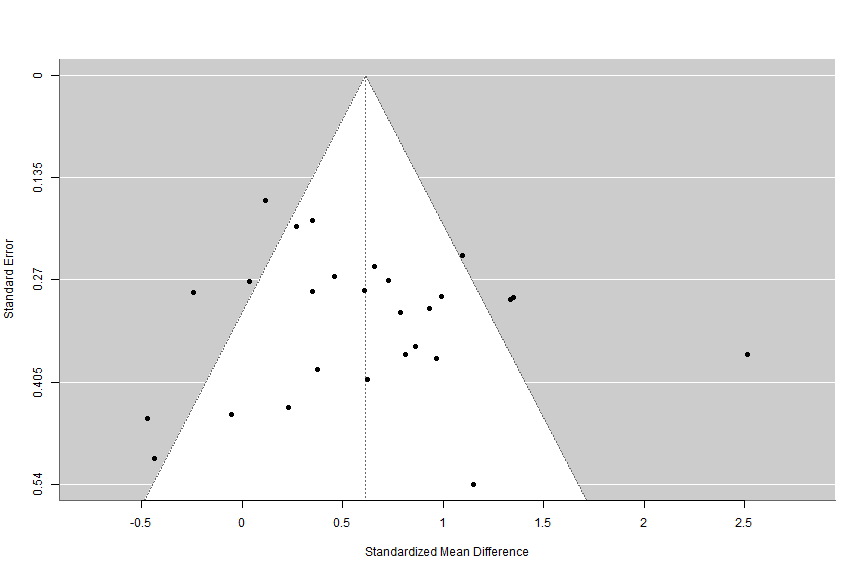
\includegraphics[width=1\textwidth,height=\textheight]{images/clipboard-27399461.png}
\caption{Now when we examine that funnel plot, it is not perfectly symmetrical, but it also isn't too crazy. For the purposes of this example we'll say that it is reasonably symmetrical.}
\end{figure}

\hypertarget{trim-and-fill-analysis}{%
\subsubsection{Trim and Fill Analysis}\label{trim-and-fill-analysis}}

Next we'll check out a trim and fill analysis to see what it finds.

\begin{Shaded}
\begin{Highlighting}[]
\CommentTok{\# carry out trim{-}and{-}fill analysis}
\NormalTok{trimandfill }\OtherTok{\textless{}{-}} \FunctionTok{trimfill}\NormalTok{(overallresult)}
\NormalTok{trimandfill}
\end{Highlighting}
\end{Shaded}

\emph{What's this code doing?}

First we are creating a new item, which we call `\textbf{trimandfill}'. Then we use the \textbf{trimfill} function with the data from the overall meta-analysis result.

The second line of code simply displays the results.

Running that code gives us the following results in our console:

\begin{Shaded}
\begin{Highlighting}[]
\NormalTok{Estimated number of missing studies on the right side}\SpecialCharTok{:} \DecValTok{2}\NormalTok{ (}\AttributeTok{SE =} \FloatTok{3.3967}\NormalTok{)}

\NormalTok{Random}\SpecialCharTok{{-}}\NormalTok{Effects }\FunctionTok{Model}\NormalTok{ (}\AttributeTok{k =} \DecValTok{29}\NormalTok{; tau}\SpecialCharTok{\^{}}\DecValTok{2}\NormalTok{ estimator}\SpecialCharTok{:}\NormalTok{ REML)}

\NormalTok{tau}\SpecialCharTok{\^{}}\DecValTok{2}\NormalTok{ (estimated amount of total heterogeneity)}\SpecialCharTok{:} \FloatTok{0.2780}\NormalTok{ (}\AttributeTok{SE =} \FloatTok{0.1034}\NormalTok{)}
\FunctionTok{tau}\NormalTok{ (square root of estimated tau}\SpecialCharTok{\^{}}\DecValTok{2}\NormalTok{ value)}\SpecialCharTok{:}      \FloatTok{0.5273}
\NormalTok{I}\SpecialCharTok{\^{}}\DecValTok{2}\NormalTok{ (total heterogeneity }\SpecialCharTok{/}\NormalTok{ total variability)}\SpecialCharTok{:}   \FloatTok{75.67}\NormalTok{\%}
\NormalTok{H}\SpecialCharTok{\^{}}\DecValTok{2}\NormalTok{ (total variability }\SpecialCharTok{/}\NormalTok{ sampling variability)}\SpecialCharTok{:}  \FloatTok{4.11}

\NormalTok{Test }\ControlFlowTok{for}\NormalTok{ Heterogeneity}\SpecialCharTok{:}
\FunctionTok{Q}\NormalTok{(}\AttributeTok{df =} \DecValTok{28}\NormalTok{) }\OtherTok{=} \FloatTok{103.1403}\NormalTok{, p}\SpecialCharTok{{-}}\NormalTok{val }\SpecialCharTok{\textless{}}\NormalTok{ .}\DecValTok{0001}

\NormalTok{Model Results}\SpecialCharTok{:}

\NormalTok{estimate      se    zval    pval   ci.lb   ci.ub      }
  \FloatTok{0.6774}  \FloatTok{0.1161}  \FloatTok{5.8323}  \SpecialCharTok{\textless{}}\NormalTok{.}\DecValTok{0001}  \FloatTok{0.4497}  \FloatTok{0.9050}  \SpecialCharTok{**}\ErrorTok{*} 

\SpecialCharTok{{-}{-}{-}}
\NormalTok{Signif. codes}\SpecialCharTok{:}  \DecValTok{0}\NormalTok{ ‘}\SpecialCharTok{**}\ErrorTok{*}\NormalTok{’ }\FloatTok{0.001}\NormalTok{ ‘}\SpecialCharTok{**}\NormalTok{’ }\FloatTok{0.01}\NormalTok{ ‘}\SpecialCharTok{*}\NormalTok{’ }\FloatTok{0.05}\NormalTok{ ‘.’ }\FloatTok{0.1}\NormalTok{ ‘ ’ }\DecValTok{1}
\end{Highlighting}
\end{Shaded}

\emph{What's this result mean?}

The first line tells us that the analysis indicates that 2 studies may be missing from the right side of the funnel. The model results are the overall meta-analytic effect (and accompanying other data) if these two studies were imputed.

Let's also check out what the funnel plot would look like if we add the missing studies indicated by the trim and fill analysis.

\begin{Shaded}
\begin{Highlighting}[]
\CommentTok{\# draw funnel plot with missing studies filled in}
\FunctionTok{funnel}\NormalTok{(trimandfill)}
\end{Highlighting}
\end{Shaded}

\emph{What's this code doing?}

We're telling metafor to use its \textbf{funnel} function on the \textbf{trimandfill} data to create a funnel plot with the missing studies included.

When we run that code, we see the following chart in our plots:

\begin{figure}
\centering
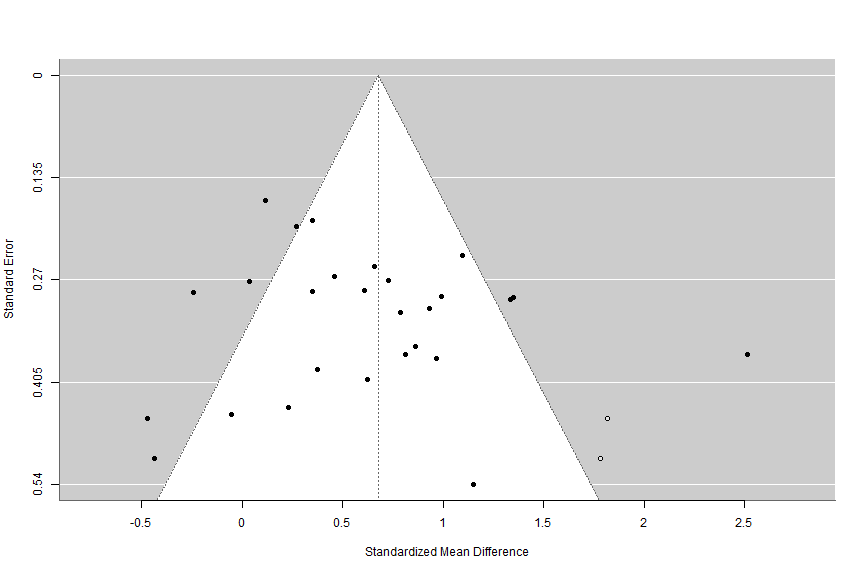
\includegraphics[width=1\textwidth,height=\textheight]{images/clipboard-2269174522.png}
\caption{This should seem very similar to your previous funnel plot - and that's because it is! Note however, the two hollow circles on the right side of the funnel (just before the 2 on the x axis). Those are our imputed studies from the trim and fill analysis.}
\end{figure}

So from the trim and fill analysis, we know that there are two studies potentially missing on the right side of the funnel. We also know that if they were included the overall meta-analytic effect size would be \emph{g} = .68. Recall that the overall meta-analytic model indicated our effect size was \emph{g} = .61. In this case, these studies absence would not notably change our overall effect size, so it is not too much of an issue. In addition, if these missing studies were included, our effect size would actually be stronger than the one we computed.

\hypertarget{eggers-regression}{%
\subsubsection{Egger's Regression}\label{eggers-regression}}

Another test we can use is Egger's regression which checks for funnel plot asymmetry. It's simple to calculate, just use the code below:

\begin{Shaded}
\begin{Highlighting}[]
\CommentTok{\#Egger\textquotesingle{}s regression}
\FunctionTok{regtest}\NormalTok{(overallresult)}
\end{Highlighting}
\end{Shaded}

What's this code doing?

This runs Egger's regression test using the data from the overall meta-analysis result.

Running that code gives us this result:

\begin{Shaded}
\begin{Highlighting}[]
\NormalTok{Regression Test }\ControlFlowTok{for}\NormalTok{ Funnel Plot Asymmetry}

\NormalTok{Model}\SpecialCharTok{:}\NormalTok{     mixed}\SpecialCharTok{{-}}\NormalTok{effects meta}\SpecialCharTok{{-}}\NormalTok{regression model}
\NormalTok{Predictor}\SpecialCharTok{:}\NormalTok{ standard error}

\NormalTok{Test }\ControlFlowTok{for}\NormalTok{ Funnel Plot Asymmetry}\SpecialCharTok{:}\NormalTok{ z }\OtherTok{=} \SpecialCharTok{{-}}\FloatTok{0.0380}\NormalTok{, p }\OtherTok{=} \FloatTok{0.9696}
\NormalTok{Limit }\FunctionTok{Estimate}\NormalTok{ (as sei }\OtherTok{{-}\textgreater{}} \DecValTok{0}\NormalTok{)}\SpecialCharTok{:}\NormalTok{   b }\OtherTok{=}  \FloatTok{0.6299}\NormalTok{ (CI}\SpecialCharTok{:} \SpecialCharTok{{-}}\FloatTok{0.2071}\NormalTok{, }\FloatTok{1.4669}\NormalTok{)}
\end{Highlighting}
\end{Shaded}

\emph{What's this result mean?}

Here we want to look at the p value. If it's less than .05, we know that there may be significant funnel plot asymmetry.

\hypertarget{fail-safe-n}{%
\subsubsection{Fail Safe N}\label{fail-safe-n}}

Some reviewers will want to see Fail Safe N tests. There are a few variants, but we'll focus on Rosenthal's Fail Safe N. This is the most common fail safe n test I see reported in the literature. We can use this code to calculate it.

\begin{Shaded}
\begin{Highlighting}[]
\CommentTok{\#Rosenthal fail safe n}
\FunctionTok{fsn}\NormalTok{(yi, vi, }\AttributeTok{data=}\NormalTok{dat1)}
\end{Highlighting}
\end{Shaded}

\emph{What's this code doing?}

This code is telling metafor to use the fail safe n function (\textbf{fsn}), referencing the effect size (\textbf{\emph{yi}}) and variance (\textbf{\emph{vi}}) from the \textbf{dat1} dataset (recall this was used to calculate our overall meta-analytic model).

When we run that code, we get the following result:

\begin{Shaded}
\begin{Highlighting}[]
\NormalTok{Fail}\SpecialCharTok{{-}}\NormalTok{safe N Calculation Using the Rosenthal Approach}

\NormalTok{Observed Significance Level}\SpecialCharTok{:} \ErrorTok{\textless{}}\NormalTok{.}\DecValTok{0001}
\NormalTok{Target Significance Level}\SpecialCharTok{:}   \FloatTok{0.05}

\NormalTok{Fail}\SpecialCharTok{{-}}\NormalTok{safe N}\SpecialCharTok{:} \DecValTok{1028}
\end{Highlighting}
\end{Shaded}

\emph{What's this result mean?}

This tells us that 1028 null effect (effect size of 0) studies would be needed to change the p value of our overall meta-analytic effect size to greater than .05.

Now, it's important to note that there are other approaches to calculating fail safe n tests, such as Orwin's and Rosenberg's. However, Rosenthal's is what I see most commonly reported.

\hypertarget{reporting-publication-bias}{%
\subsubsection{Reporting Publication Bias}\label{reporting-publication-bias}}

Ok, so we've now run a variety of tests to check for publication bias. What do they tell us, and how do we report it? Well, we know the funnel plot was reasonably symmetrical, the trim and fill only found two missing studies and they did not change our meta-analytic effect size much. Similarly, Egger's regression did not indicate significant funnel plot asymmetry. Finally, Rosenthal's fail safe n test said 1028 studies would be needed to change our overall meta-analytic effect size to be non-significant. Overall, we can state that publication bias is not likely to be a significant concern in our analysis. We can report this more specifically as follows:

\begin{quote}
We checked for the presence of publication bias using a variety of tests. First, we constructed a funnel plot. As shown in Figure 1, the funnel plot is reasonably symmetrical.

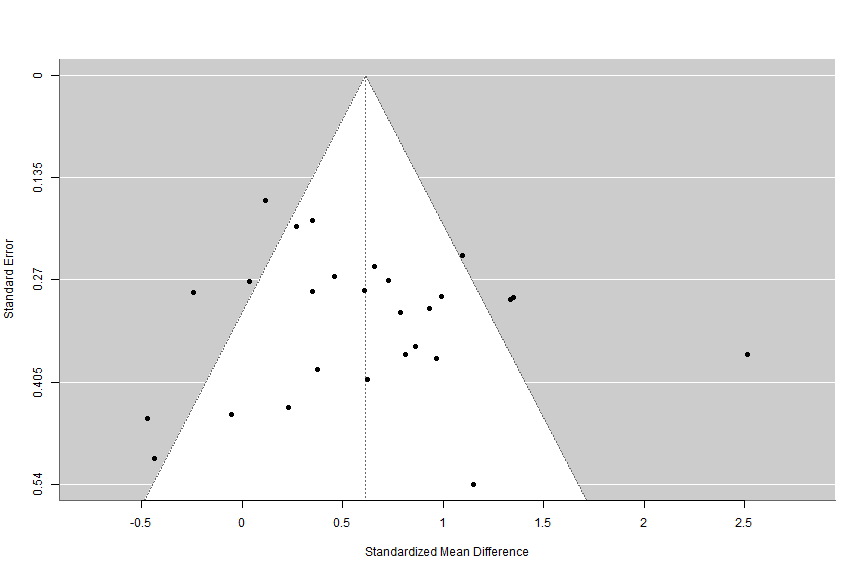
\includegraphics[width=1\textwidth,height=\textheight]{images/clipboard-27399461.png}

Next we conducted a trim and fill analysis to check for missing studies and the impact of those studies on the overall meta-analytic effect size. This test found that there were likely two studies missing on the right side of the funnel plot (Figure 2), and they would change our overall effect size to \emph{g} = .68, \emph{p} \textless{} .001. This is not notably different than the overall effect size calculated in our meta-analytic model (\emph{g} = .61, \emph{p} \textless{} .001).

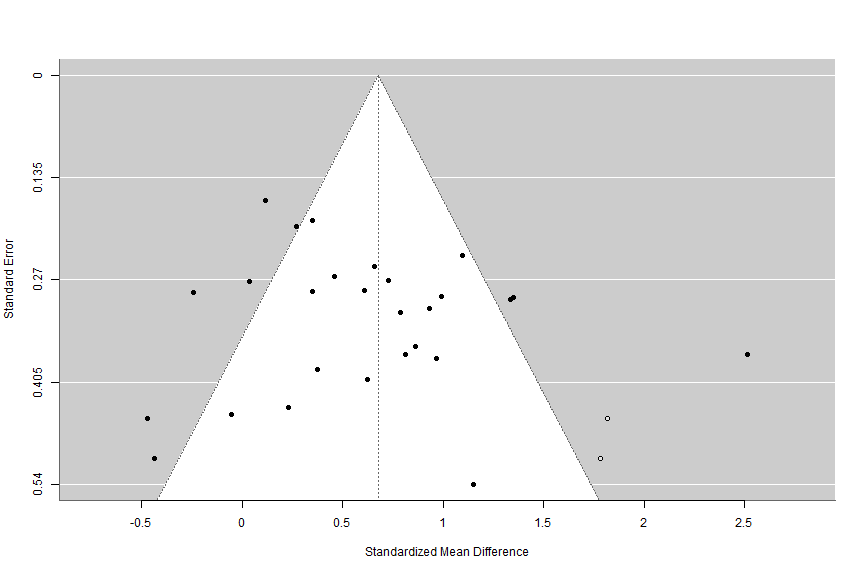
\includegraphics[width=1\textwidth,height=\textheight]{images/clipboard-2269174522.png}

Next, we used Egger's regression test to test for funnel plot asymmetry, which was not significant (z = -0.04, p = 0.97). Finally, we used Rosenthal's fail safe n test to see how many null effect studies would be needed to change the overall meta-analytic effect size to be non-significant. The test showed 1028 studies would be needed.

Based on the results of these four tests, publication bias is not expected to be a significant influence on our results.
\end{quote}

\hypertarget{thats-it}{%
\subsection{That's it!}\label{thats-it}}

You've now gone through all the steps needed to conduct a conventional meta-analysis. Congratulations! This may seem intimidating, but if you complete each step, in order, this will be a very simple process. And think - now you a) have a code you can use, with slight modifications, for every conventional meta-analysis you conduct in the future, b) have a code you can share with friends, and c) can share you code with your publication so others can replicate your analysis. Just think - if more people had done that I would not have had to write this book\ldots.

\hypertarget{section}{%
\subsubsection{}\label{section}}

\hypertarget{3LMA}{%
\chapter{Three-Level Meta-Analysis}\label{3LMA}}

This chapter will cover the basics of three-level meta-analysis in R using metafor\citep{viechtbauer2010}. Remember how in conventional meta-analysis each participant can only be counted once? Well, that means we exclude A LOT of data when we use conventional meta-analysis in many education fields. But we can use three-level meta-analysis to get around that!

Let's look at an example: Say you are comparing the impact of learning from a virtual character to a game on learning outcomes. The study you're coding has two groups, a virtual character group and a game group. It has an immediate learning test, a one week delayed learning test, and a month delayed learning test. Which test do you code? In a three-level meta-analysis, you can code all three! No data lost, yay!

As noted in the conventional meta-analysis chapter, we're focusing on random-effects models here. If you don't know the differences between fixed and random effects meta-analysis models, please see \citep{borenstein2010}.

If you aren't familiar with conventional meta-analysis, please read about it before conducting any meta-analysis. There are plenty of free resources available. I would recommend starting with the great, free book, \href{https://bookdown.org/MathiasHarrer/Doing_Meta_Analysis_in_R/}{Doing Meta-Analysis in R}\citep{harrer2021}. This same book explains three-level meta-analysis quite well too!

Let's say you understand the differences between conventional and three-level meta-analytic models, you understand what meta-analysis is used for, and you've decided you're moving ahead with the three-level model. Let's explore how to do this in R with metafor using standardized mean differences as the effect size.

\hypertarget{preparing-your-data-1}{%
\section{Preparing your data}\label{preparing-your-data-1}}

Hopefully you have already run your \protect\hyperlink{crossliteraturesearch}{literature search}, \protect\hyperlink{crossscreening}{screened your studies}, and \protect\hyperlink{crossdata}{extracted your data}. This point forward assumes you have already completed these steps.

\hypertarget{your-data-file-1}{%
\subsection{Your Data File}\label{your-data-file-1}}

Personally I prefer to use .csv files as my data file that I import into R. Why? Because that's what was always used in the examples I found online when I was learning R, and I've used it ever since. Why change something that works? Plus, .csv works with many different software programs and across various operating systems. ~

As noted in the \protect\hyperlink{crossdata}{data extraction and coding chapter}, metafor uses two pieces of information for conducting the meta-analysis that you need to consider before importing data in R: the effect size (\textbf{\emph{yi}}) and the variance (\textbf{\emph{vi}}). If you read the previous chapters, you know you have choices when coding: you can code the mean, standard deviation, and sample size for the experimental and control groups and then use R and metafor to calculate the effect size and variance for each comparison (my recommended method), or you can calculate the effect size and variance for each effect size yourself. I prefer the former approach because I find it helpful to have all of this data to not only check for errors in coding (such as a misplaced decimal point -- these things happen!) and also for calculating sample sizes for tables.

If you choose to use R and metafor to calculate the effect sizes and variance, it will be important to have each mean, standard deviation, and sample size for the experimental group and the control group in their own columns. I recommend having simple column titles that are descriptive and easy to remember, because you will have to type them into R. \textbf{See a sample coding form below that we will use to complete this analysis}. Note that you can have as many moderator variables as you wish, and they can be continuous or categorical.

\textbf{Important Reminder:}

Preparing your data looks very similar to a conventional meta-analysis. However, it is important that you have two columns that are formatted in a specific way. First, you need a column that simply labels each comparison with a number that is not duplicative of any other comparison. In other words, you can simply code all your data, then create a new column and label each respective comparison as 1, 2, 3, 4, etc.

Second is the study column. It is important that every comparison from the same study appears the same. To avoid issues here, I recommend copy-pasting.

So in the end, your coding form may look like this, which contains three effect sizes from one study:

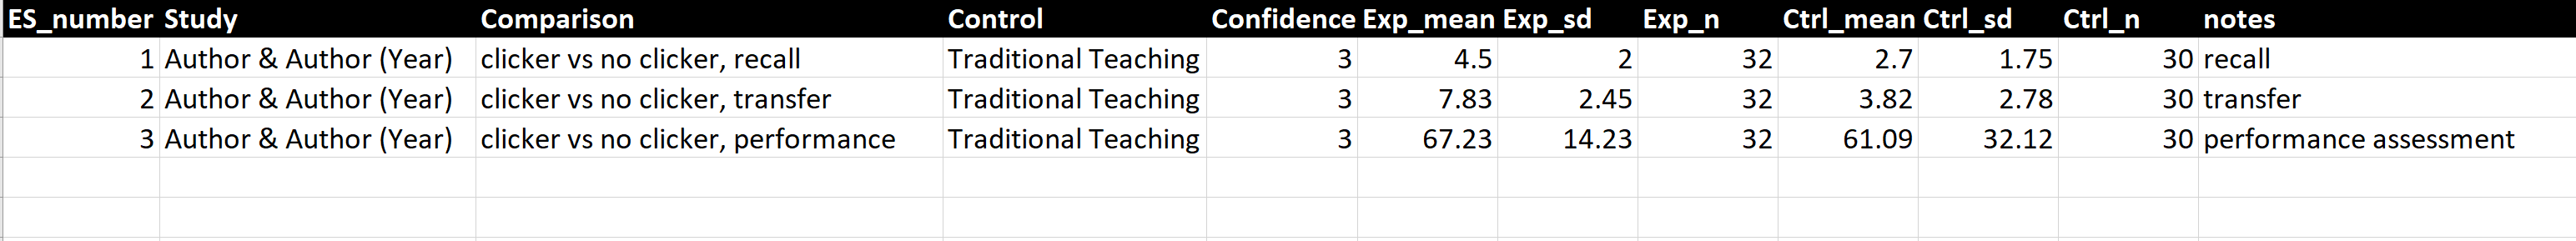
\includegraphics[width=2\textwidth,height=\textheight]{images/3lmacoding.PNG}

So, assuming you have all of that done, let's get onto the fun stuff, running a three-level meta-analysis!

\hypertarget{running-a-three-level-meta-analysis-in-metafor}{%
\section{Running a Three-Level Meta-Analysis in Metafor}\label{running-a-three-level-meta-analysis-in-metafor}}

\hypertarget{example-data-for-this-analysis-1}{%
\subsection{Example Data for This Analysis}\label{example-data-for-this-analysis-1}}

If you want to follow along with this specific example, you'll want to use the subset of data from Schroeder et al.'s (2023)\citep{schroeder2023} meta-analysis on the effects of 360˚ video on learning. The data can be downloaded here.

\hypertarget{load-r-packages-1}{%
\subsection{Load R Packages}\label{load-r-packages-1}}

First we need to load our R packages. Hopefully you installed these already, if not it won't take long, just see the \protect\hyperlink{crossrpackages}{R Basics chapter}. Assuming you have already installed the R packages, let's load them up so we can do some analysis!

\begin{Shaded}
\begin{Highlighting}[]
\DocumentationTok{\#\#\#\#\#\#\#\#\#\#\#\#\#\#\#\#\#\#\#\#\#\#\#\#\#\#\#}
\CommentTok{\#Preparation\#}
\DocumentationTok{\#\#\#\#\#\#\#\#\#\#\#\#\#\#\#\#\#\#\#\#\#\#\#\#\#\#\#}

\CommentTok{\#load packages}
\FunctionTok{library}\NormalTok{(metafor)}
\FunctionTok{library}\NormalTok{(ggplot2)}
\FunctionTok{library}\NormalTok{(dplyr)}
\end{Highlighting}
\end{Shaded}

\emph{What's this code doing?}

This code is simply loading the metafor, ggplot2, and dplyr packages in the R environment so we can do our analysis.

\hypertarget{import-your-data-into-r-studio-1}{%
\subsection{Import Your Data Into R Studio}\label{import-your-data-into-r-studio-1}}

The first step to conducting your meta-analysis is to read in the data. To do that, we first want to set our working directory (more about that in the \protect\hyperlink{crossrbasics}{R Basics chapter}). Once you've set your working directory, you can use this piece of code.

\begin{Shaded}
\begin{Highlighting}[]
\CommentTok{\#name data file and read in .csv.}
\NormalTok{df }\OtherTok{\textless{}{-}} \FunctionTok{read.csv}\NormalTok{(}\StringTok{"360 sample data.csv"}\NormalTok{)}
\end{Highlighting}
\end{Shaded}

\emph{What's this code doing?\\
}You see the first piece of code is `\textbf{df}', which is what we are going to name our data file. The \textbf{\textless-} indicates that you are going to name something. The next piece is telling R to read in a .csv file from the working directory, and then you can see the file name I used. So basically, we're saying \emph{import this data and call it df}.

\hypertarget{calculating-effect-sizes-1}{%
\subsection{Calculating Effect Sizes}\label{calculating-effect-sizes-1}}

Next, you will want to calculate the effect sizes and variance for each effect size if you have not done so already. You can do that using this code:

\begin{Shaded}
\begin{Highlighting}[]
\NormalTok{dat1 }\OtherTok{\textless{}{-}} \FunctionTok{escalc}\NormalTok{(}\AttributeTok{measure=}\StringTok{"SMD"}\NormalTok{, }\AttributeTok{m1i=}\NormalTok{Exp\_mean, }\AttributeTok{sd1i=}\NormalTok{Exp\_sd, }\AttributeTok{n1i=}\NormalTok{Exp\_n,}
               \AttributeTok{m2i=}\NormalTok{Ctrl\_mean, }\AttributeTok{sd2i=}\NormalTok{Ctrl\_sd, }\AttributeTok{n2i=}\NormalTok{Ctrl\_n, }\AttributeTok{data=}\NormalTok{df)}
\end{Highlighting}
\end{Shaded}

\emph{What's this code doing?}

\textbf{dat1 \textless-} indicates naming a new datafile and we're calling it \textbf{dat1}.

In this case you're doing a calculation. \textbf{Escalc} is telling it calculate an effect size, \textbf{measure=``SMD''} is saying we want the effect sizes to be standardized mean differences.

The next set of variables (\textbf{m1i, sd1i, n1i, m2i, sd2i,} and \textbf{n2i}) are specific pieces of information that metafor needs to calculate the effect size. \textbf{m1i} is the mean of the intervention group. \textbf{sd1i} is the standard deviation of the intervention group. \textbf{n1i} is the sample size of the intervention group. \textbf{m2i} is the mean of the control group. \textbf{sd2i} is the standard deviation of the control group. \textbf{n2i} is the sample size of the control group. I have always found those codes hard to remember, so on my coding form/data file I use different column headings. You can see I tell metafor where to find each variable by using the \textbf{=} sign. For example, the mean of the intervention group (\textbf{m1i}) is called \textbf{Exp\_mean} in my data file.

Finally, we need to tell metafor where to find the data, and we have to refer to data already in R. We use our datafile `\textbf{df}'.

Now you can make sure the effect size and variance for each effect size were calculated:

\begin{Shaded}
\begin{Highlighting}[]
\CommentTok{\#display dataset with ES and variance}
\NormalTok{dat1}
\end{Highlighting}
\end{Shaded}

\emph{What's this code doing?}

This will display your full data set saved as `\textbf{dat1}' in the console.

However, I find this kind of hard to read if I have a lot of data. So, I prefer to write it all to a .csv file instead because I find it easier to read. This code can do that:

\begin{Shaded}
\begin{Highlighting}[]
\CommentTok{\#save .csv file with ES data. This goes into working directory}
\FunctionTok{write.csv}\NormalTok{(dat1, }\AttributeTok{file =} \StringTok{"ESdata.csv"}\NormalTok{)}
\end{Highlighting}
\end{Shaded}

\emph{What's this code doing?}

The \textbf{write.csv} tells R you want to create a .csv file. This will be saved in your working directory.

The \textbf{dat1} is telling R which data you want to write into the .csv file.

\textbf{File = ``ESdata.csv''} is simply naming the datafile between the '' ``. You can name it whatever you want, but my example will use ESdata as the file name.

You're probably wondering, \emph{Why write a .csv file with the effect size and variance data when it is saved in R?}

Well, I like to look at the .csv file and make sure I don't see any effect sizes that seem very wrong. If I find any then it is easy for me to track back to which study it came from and I can see if I made a mistake during coding. A misplaced decimal point can have huge implications for your analysis - this is a step that helps you catch those human errors.

\hypertarget{running-the-meta-analysis-model-1}{%
\section{Running The Meta-Analysis Model}\label{running-the-meta-analysis-model-1}}

Now the part we've all been waiting for, let's run a three-level meta-analysis model! We can use this code:

\begin{Shaded}
\begin{Highlighting}[]
\CommentTok{\#multilevel model}
\NormalTok{m\_multi }\OtherTok{\textless{}{-}} \FunctionTok{rma.mv}\NormalTok{(yi,}
\NormalTok{                  vi,}
                  \AttributeTok{random =} \SpecialCharTok{\textasciitilde{}} \DecValTok{1} \SpecialCharTok{|}\NormalTok{ Study}\SpecialCharTok{/}\NormalTok{ES\_number,}
                  \AttributeTok{method =} \StringTok{"REML"}\NormalTok{,}
                  \AttributeTok{test =} \StringTok{"t"}\NormalTok{,}
                  \AttributeTok{dfs =} \StringTok{"contain"}\NormalTok{,}
                  \AttributeTok{data =}\NormalTok{ dat1) }
\NormalTok{m\_multi}
\end{Highlighting}
\end{Shaded}

\emph{What's this code doing?}

This looks scary doesn't it? It's not that complicated actually. Let's see what we're doing with this code.

First, we're naming our meta-analysis result as a new piece of data in R, and we're naming it `\textbf{m\_multi}'

\textbf{rma.mv} is telling metafor that we want to run a random-effects, multivariate meta-analysis model. Within that, we're using \textbf{yi} to reference effect size data within our data set, \textbf{vi} to reference effect size variance within our data set.

The next line is a bit more complex. Harrer et al.~(2021)\citep{harrer2021} explain that this is used to define the random effects and their nesting. Specifically, we will always start with \textbf{\textasciitilde1 and a vertical bar} for three-level models. Next, we need to define what our grouping variables are, in our case, it's going to be studies (\textbf{Study} column in our data set), and within studies, are effect size numbers (\textbf{ES\_number} column in our data set).

\textbf{method} is specifying that we want to use Restricted Maximum-Likelihood.

\textbf{test}, by default, uses z. However Harrer et al.~(2021)\citep{harrer2021} recommend using `\textbf{t}' because it is similar to the Knapp-Hartung method.

\textbf{dfs = ``contain''} is done because using ``residual'' can lead to inflated Type 1 error rate according to Viechtbauer (n.d.)\citep{viechtbauer}.

and \textbf{data = dat1} is simply telling metafor which data set within R to reference when running the analysis.

Finally, \textbf{m\_multi} displays the analysis results on the screen.

\hypertarget{interpreting-the-results-1}{%
\subsection{Interpreting the Results}\label{interpreting-the-results-1}}

When we run that code, we now see the following:

\begin{Shaded}
\begin{Highlighting}[]
\NormalTok{Multivariate Meta}\SpecialCharTok{{-}}\NormalTok{Analysis }\FunctionTok{Model}\NormalTok{ (}\AttributeTok{k =} \DecValTok{35}\NormalTok{; method}\SpecialCharTok{:}\NormalTok{ REML)}

\NormalTok{Variance Components}\SpecialCharTok{:}

\NormalTok{            estim    sqrt  nlvls  fixed           factor }
\NormalTok{sigma}\SpecialCharTok{\^{}}\FloatTok{2.1}  \FloatTok{2.6808}  \FloatTok{1.6373}     \DecValTok{12}\NormalTok{     no            Study }
\NormalTok{sigma}\SpecialCharTok{\^{}}\FloatTok{2.2}  \FloatTok{0.1649}  \FloatTok{0.4061}     \DecValTok{35}\NormalTok{     no  Study}\SpecialCharTok{/}\NormalTok{ES\_number }

\NormalTok{Test }\ControlFlowTok{for}\NormalTok{ Heterogeneity}\SpecialCharTok{:}
\FunctionTok{Q}\NormalTok{(}\AttributeTok{df =} \DecValTok{34}\NormalTok{) }\OtherTok{=} \FloatTok{285.5500}\NormalTok{, p}\SpecialCharTok{{-}}\NormalTok{val }\SpecialCharTok{\textless{}}\NormalTok{ .}\DecValTok{0001}

\NormalTok{Model Results}\SpecialCharTok{:}

\NormalTok{estimate      se     tval  df    pval    ci.lb   ci.ub    }
 \SpecialCharTok{{-}}\FloatTok{0.3799}  \FloatTok{0.4843}  \SpecialCharTok{{-}}\FloatTok{0.7843}  \DecValTok{11}  \FloatTok{0.4494}  \SpecialCharTok{{-}}\FloatTok{1.4459}  \FloatTok{0.6861}    

\SpecialCharTok{{-}{-}{-}}
\NormalTok{Signif. codes}\SpecialCharTok{:}  \DecValTok{0}\NormalTok{ ‘}\SpecialCharTok{**}\ErrorTok{*}\NormalTok{’ }\FloatTok{0.001}\NormalTok{ ‘}\SpecialCharTok{**}\NormalTok{’ }\FloatTok{0.01}\NormalTok{ ‘}\SpecialCharTok{*}\NormalTok{’ }\FloatTok{0.05}\NormalTok{ ‘.’ }\FloatTok{0.1}\NormalTok{ ‘ ’ }\DecValTok{1}
\end{Highlighting}
\end{Shaded}

\emph{What's this mean?}

Recall this is a subset of data from Schroeder et al.~(2023)\citep{schroeder2023} so the numbers will not align with what is in the published version.

The first line tells us this is a multivariate random-effects model including 35 comparisons, and tau\textsuperscript{2} was estimated using restricted maximum likelihood estimation (REML).

Next, we see our variance components. The estimate is tau\textsuperscript{2}. The first (\textbf{sigma2.1}) refers to the between-study heterogeneity, whereas \textbf{sigma2.2} refers to within-comparison heterogeneity.

Typically, the other important pieces here that we are interested in reporting in our manuscript are the \textbf{overall effect size, tau\textsuperscript{2}}, and the \textbf{\emph{Q}-test}.

The \textbf{effect size} (model results in this output) is interpreted as the standardized mean difference effect size, if there is a significant \emph{Q} test it indicates there is significant heterogeneity in our sample.

Next, let's check out the variance components in more depth.

\hypertarget{explaining-the-variance}{%
\subsection{Explaining the Variance}\label{explaining-the-variance}}

In the above step, we saw tau\textsuperscript{2}, but we did not see \emph{I}\textsuperscript{2}. If you're familiar with conventional meta-analysis, you know that \emph{I}\textsuperscript{2} tells us how much variation is explained by between-study heterogeneity. In three-level meta-analysis we can look at this to find both a within-study and between-comparison value. Let's check out that code:

\textbf{Important:} First, we actually need to do some background work. Harrer et al.~(2021)\citep{harrer2021} have provided code that helps us calculate \emph{I}\textsuperscript{2},but first we need to `teach' R that analysis.

So, please visit this link and copy the entire code: \url{https://raw.githubusercontent.com/MathiasHarrer/dmetar/master/R/mlm.variance.distribution.R}

Got the code? Great, go ahead and paste that into the R \ul{console} (where your results are usually displayed in R studio) and \textbf{hit enter.} Awesome, now R knows the analysis.

Now we can use this code to calculate \emph{I}\textsuperscript{2}.

\begin{Shaded}
\begin{Highlighting}[]
\CommentTok{\#calculate i2 for each level}
\NormalTok{i2 }\OtherTok{\textless{}{-}} \FunctionTok{var.comp}\NormalTok{(m\_multi)}
\FunctionTok{summary}\NormalTok{(i2)}
\NormalTok{i2}
\end{Highlighting}
\end{Shaded}

\emph{What's this code doing?}

We are creating a new object, \textbf{i2}, and using the function \textbf{var.comp} on our overall meta-analysis model (\textbf{m\_multi}).

Then we calculate \textbf{summary} statistics for i2.

And finally display i2 on the screen.

Let's look at the results:

\begin{Shaded}
\begin{Highlighting}[]
\SpecialCharTok{$}\NormalTok{results}
\NormalTok{        \% of total variance    I2}
\NormalTok{Level }\DecValTok{1}            \FloatTok{2.805362}   \SpecialCharTok{{-}{-}{-}}
\NormalTok{Level }\DecValTok{2}            \FloatTok{5.631495}  \FloatTok{5.63}
\NormalTok{Level }\DecValTok{3}           \FloatTok{91.563144} \FloatTok{91.56}

\SpecialCharTok{$}\NormalTok{totalI2}
\NormalTok{[}\DecValTok{1}\NormalTok{] }\FloatTok{97.19464}
\end{Highlighting}
\end{Shaded}

\emph{What's this result mean?}

When you run this analysis, you'll see that 5.63\% of the variance is due to level 2 (within-study) heterogeneity, while 91.56\% is due to between-comparisons heterogeneity. Overall, the model explains 97.2\% of the variance.

We can also get the same information from the plot that was generated:

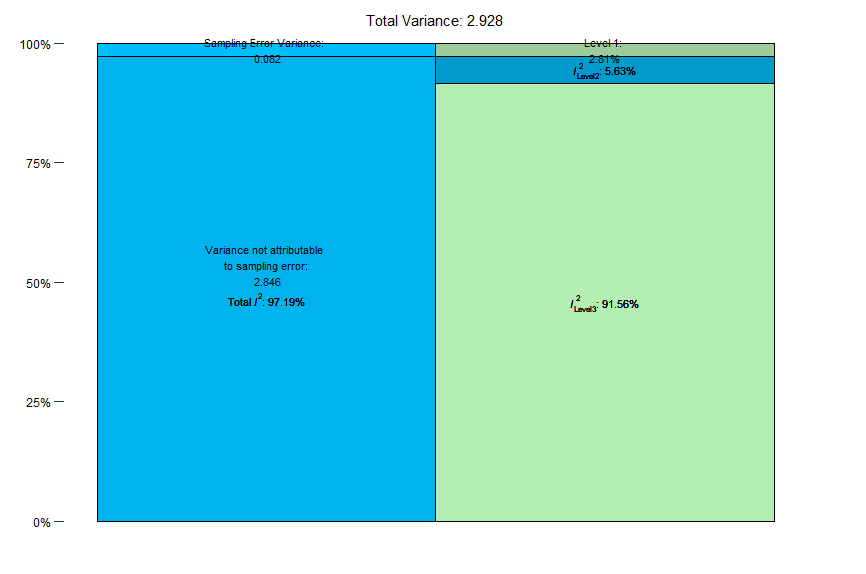
\includegraphics[width=1\textwidth,height=\textheight]{images/i2plot.png}

Ok, so we've established that we have quite a bit of between-comparison heterogeneity. When we consider that the tau\textsuperscript{2} for the between-comparison heterogeneity was notably higher than the within-study heterogeneity, these results are consistent and help us rationalize conducting moderator analyses.

\hypertarget{checking-for-outliers-and-influence-1}{%
\subsection{Checking for Outliers and Influence}\label{checking-for-outliers-and-influence-1}}

At this point we've ran our random-effects three-level meta-analysis model. We also understand where the variance is coming from. However, we have not checked for outliers or studies with significant influence on the results. This is actually a complex topic, as not many meta-analyses (as of January, 2024) in education actually address a) if they searched for outliers or influence, b) what metric they used to check for outliers and why, and c) what they did about the outliers and why. Kind of interesting right?

So here's what we can do to check for outliers and influence. Unfortunately it isn't quite as easy as evaluating outliers in conventional meta-analysis, but don't worry, it's not too difficult!

First, let's check for outliers. We're going to slightly adapt Van Lissa's (n.d.)\citep{vanlissa} method.

\begin{Shaded}
\begin{Highlighting}[]
\CommentTok{\#adapting CI calculation and plotting from https://cjvanlissa.github.io/Doing{-}Meta{-}Analysis{-}in{-}R/detecting{-}outliers{-}influential{-}cases.html}
\CommentTok{\# Calculate CI for all observed effect sizes}
\NormalTok{dat1}\SpecialCharTok{$}\NormalTok{upperci }\OtherTok{\textless{}{-}}\NormalTok{ dat1}\SpecialCharTok{$}\NormalTok{yi }\SpecialCharTok{+} \FloatTok{1.96} \SpecialCharTok{*} \FunctionTok{sqrt}\NormalTok{(dat1}\SpecialCharTok{$}\NormalTok{vi)}
\NormalTok{dat1}\SpecialCharTok{$}\NormalTok{lowerci }\OtherTok{\textless{}{-}}\NormalTok{ dat1}\SpecialCharTok{$}\NormalTok{yi }\SpecialCharTok{{-}} \FloatTok{1.96} \SpecialCharTok{*} \FunctionTok{sqrt}\NormalTok{(dat1}\SpecialCharTok{$}\NormalTok{vi)}
\CommentTok{\# Create filter variable}
\NormalTok{dat1}\SpecialCharTok{$}\NormalTok{outlier }\OtherTok{\textless{}{-}}\NormalTok{ dat1}\SpecialCharTok{$}\NormalTok{upperci }\SpecialCharTok{\textless{}}\NormalTok{ m\_multi}\SpecialCharTok{$}\NormalTok{ci.lb }\SpecialCharTok{|}\NormalTok{ dat1}\SpecialCharTok{$}\NormalTok{lowerci }\SpecialCharTok{\textgreater{}}\NormalTok{ m\_multi}\SpecialCharTok{$}\NormalTok{ci.ub}
\CommentTok{\# Count number of outliers:}
\FunctionTok{sum}\NormalTok{(dat1}\SpecialCharTok{$}\NormalTok{outlier)}
\NormalTok{dat1}
\CommentTok{\# Make a basic plot, based on the data in dat1, and specify that the x{-}variable is the effect size, \textquotesingle{}d\textquotesingle{}, the colour and fill of the histogram bars are based on}
\CommentTok{\# the value of \textquotesingle{}outlier\textquotesingle{}:}
\FunctionTok{ggplot}\NormalTok{(}\AttributeTok{data =}\NormalTok{ dat1, }\FunctionTok{aes}\NormalTok{(}\AttributeTok{x =}\NormalTok{ yi, }\AttributeTok{colour =}\NormalTok{ outlier, }\AttributeTok{fill =}\NormalTok{ outlier)) }\SpecialCharTok{+}
  \CommentTok{\# Add a histogram with transparent bars (alpha = .2)}
  \FunctionTok{geom\_histogram}\NormalTok{(}\AttributeTok{alpha =}\NormalTok{ .}\DecValTok{2}\NormalTok{) }\SpecialCharTok{+}
  \CommentTok{\# Add a vertical line at the pooled effect value (m\_re$b[1])}
  \FunctionTok{geom\_vline}\NormalTok{(}\AttributeTok{xintercept =}\NormalTok{ m\_multi}\SpecialCharTok{$}\NormalTok{b[}\DecValTok{1}\NormalTok{]) }\SpecialCharTok{+}
  \CommentTok{\# Apply a black and white theme}
  \FunctionTok{theme\_bw}\NormalTok{()}

\DocumentationTok{\#\#Print file that lists outliers. This goes into working directory}
\FunctionTok{write.csv}\NormalTok{(dat1, }\AttributeTok{file =} \StringTok{"outliers indicated.csv"}\NormalTok{)}
\end{Highlighting}
\end{Shaded}

\emph{What's this code doing?}

This code identifies outliers using the criteria that the individual effect size's confidence interval does not overlap the meta-analytical effect size confidence interval. It creates a nice chart that you'll see appear in your plots, and it will create a .csv file with outliers indicated.

Running that code created a plot, a .csv file, and displayed data in the console. I prefer to first examine the plot, which shows three outliers in blue.

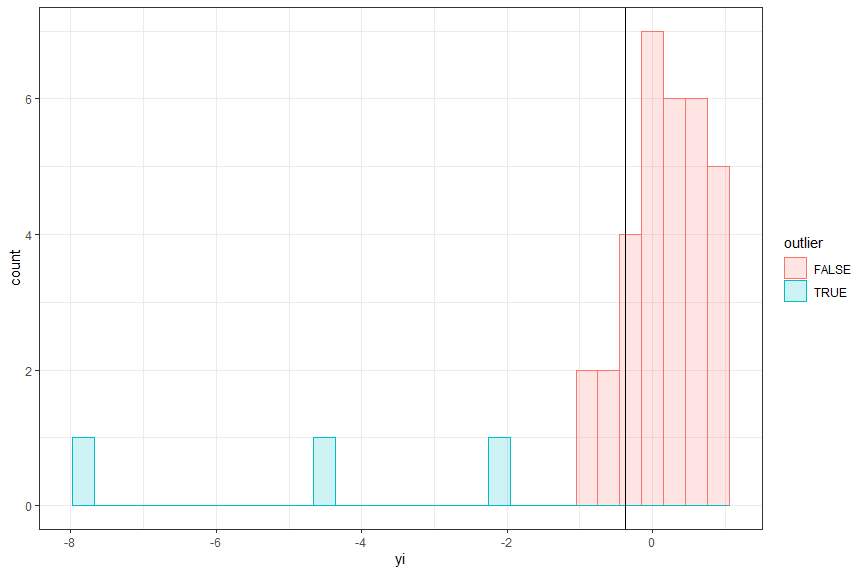
\includegraphics[width=1\textwidth,height=\textheight]{images/outliers3level.png}

You can see here with have three outliers using this criteria, however we don't know which comparisons they are. Both the data in the console and generated .csv file tell us which comparisons were outliers.

At this point, similar to conventional meta-analysis, we need to examine the studies in more detail. First, I check for any data entry errors. Sometimes decimal points are in the wrong place, which can easy create an outlier.

\hypertarget{checking-for-influence}{%
\subsubsection{Checking for Influence}\label{checking-for-influence}}

Assuming there were no data entry errors, I then move on to check and see if these outliers have a significant influence on the results. Similar to conventional meta-analysis, we're going to examine Cook's distance, dfbetas, and hat values. You can read about influence diagnostics and the metrics used \href{https://wviechtb.github.io/metafor/reference/influence.rma.mv.html}{here} and in Viechtbauer and Cheung (2010)\citep{viechtbauer2010b}.Unfortunately, we're not using the nice influence code that provided asterisks on influential studies, so we'll have to a do a bit of work ourselves.

\hypertarget{cooks-distance}{%
\paragraph{Cook's Distance}\label{cooks-distance}}

First, let's check out the Cook's distance.

\begin{Shaded}
\begin{Highlighting}[]
\CommentTok{\#cook\textquotesingle{}s distance}
\NormalTok{cooks }\OtherTok{\textless{}{-}} \FunctionTok{cooks.distance}\NormalTok{(m\_multi)}
\FunctionTok{plot}\NormalTok{(cooks, }\AttributeTok{type=}\StringTok{"o"}\NormalTok{, }\AttributeTok{pch=}\DecValTok{19}\NormalTok{, }\AttributeTok{xlab=}\StringTok{"Observed Outcome"}\NormalTok{, }\AttributeTok{ylab=}\StringTok{"Cook\textquotesingle{}s Distance"}\NormalTok{)}
\end{Highlighting}
\end{Shaded}

\emph{What's this code doing?}

This code calculates Cook's distance based on our overall meta-analysis result (\textbf{m\_multi}).

Running that code gives us the following plot:

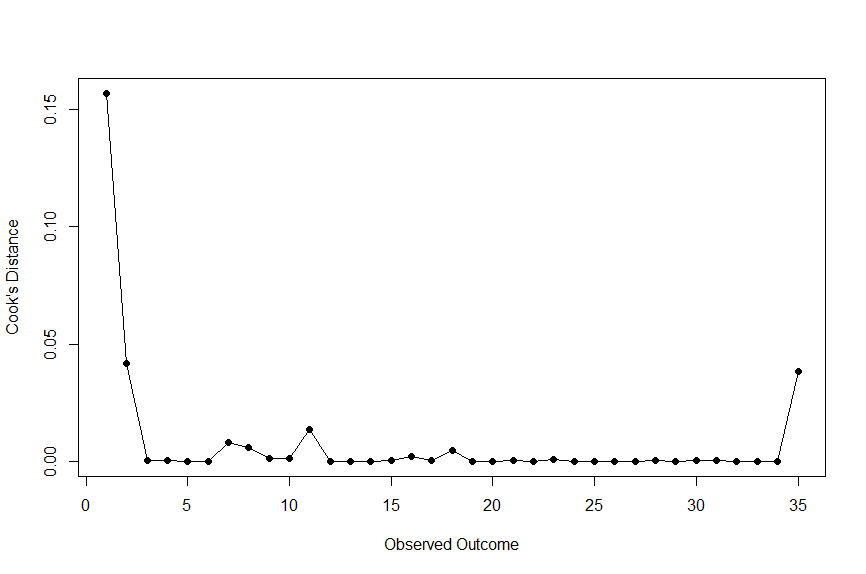
\includegraphics[width=1\textwidth,height=\textheight]{images/cook3level.png}

Here, we are looking for a Cook's distance over 0.50 to indicate a study with significant influence. As shown, none of our outliers meet this criteria.

\hypertarget{dfbetas}{%
\paragraph{dfbetas}\label{dfbetas}}

Now let's check our dfbetas. Here's the code:

\begin{Shaded}
\begin{Highlighting}[]
\CommentTok{\#Calculate dfbetas}
\NormalTok{dfbetas }\OtherTok{\textless{}{-}}\FunctionTok{dfbetas}\NormalTok{(m\_multi)}
\NormalTok{dfbetas }
\end{Highlighting}
\end{Shaded}

\emph{What's this code doing?}

Here we are creating a \textbf{dfbetas} item, and using the \textbf{dfbetas} function on our meta-analytic model (\textbf{m\_multi}).

We then display the results in the console.

This gives us the following results:

\begin{Shaded}
\begin{Highlighting}[]
\NormalTok{        intrcpt}
\DecValTok{1}  \SpecialCharTok{{-}}\FloatTok{0.626210184}
\DecValTok{2}   \FloatTok{0.169860526}
\DecValTok{3}  \SpecialCharTok{{-}}\FloatTok{0.019773230}
\DecValTok{4}   \FloatTok{0.018578841}
\DecValTok{5}   \FloatTok{0.006064717}
\DecValTok{6}   \FloatTok{0.005999710}
\DecValTok{7}  \SpecialCharTok{{-}}\FloatTok{0.089768522}
\DecValTok{8}   \FloatTok{0.075905014}
\DecValTok{9}  \SpecialCharTok{{-}}\FloatTok{0.036595130}
\DecValTok{10}  \FloatTok{0.032405437}
\DecValTok{11}  \FloatTok{0.110392454}
\DecValTok{12} \SpecialCharTok{{-}}\FloatTok{0.004587048}
\DecValTok{13} \SpecialCharTok{{-}}\FloatTok{0.007298008}
\DecValTok{14} \SpecialCharTok{{-}}\FloatTok{0.001561507}
\DecValTok{15}  \FloatTok{0.021281904}
\DecValTok{16} \SpecialCharTok{{-}}\FloatTok{0.044837905}
\DecValTok{17} \SpecialCharTok{{-}}\FloatTok{0.019897092}
\DecValTok{18}  \FloatTok{0.067207219}
\DecValTok{19}  \FloatTok{0.003352683}
\DecValTok{20}  \FloatTok{0.007897610}
\DecValTok{21} \SpecialCharTok{{-}}\FloatTok{0.016373463}
\DecValTok{22}  \FloatTok{0.002410328}
\DecValTok{23}  \FloatTok{0.029562056}
\DecValTok{24} \SpecialCharTok{{-}}\FloatTok{0.010640162}
\DecValTok{25}  \FloatTok{0.009266463}
\DecValTok{26}  \FloatTok{0.005062508}
\DecValTok{27} \SpecialCharTok{{-}}\FloatTok{0.003420734}
\DecValTok{28}  \FloatTok{0.015525088}
\DecValTok{29} \SpecialCharTok{{-}}\FloatTok{0.007364825}
\DecValTok{30}  \FloatTok{0.012981876}
\DecValTok{31} \SpecialCharTok{{-}}\FloatTok{0.014656427}
\DecValTok{32}  \FloatTok{0.012061267}
\DecValTok{33} \SpecialCharTok{{-}}\FloatTok{0.011572638}
\DecValTok{34} \SpecialCharTok{{-}}\FloatTok{0.001067083}
\DecValTok{35}  \FloatTok{0.189468678}
\end{Highlighting}
\end{Shaded}

\emph{What's this result mean?}

Here, we're looking for values more than the absolute value of 1. If those exist (none do in this data) we know that comparison has a significant influence on the results.

\hypertarget{hat-values}{%
\paragraph{Hat values}\label{hat-values}}

Finally we can check hat values to help us check for studies with significant influence on the overall meta-analytical result. We'll use this code:

\begin{Shaded}
\begin{Highlighting}[]
\CommentTok{\#calculate hatvalues}
\NormalTok{hatvalues }\OtherTok{\textless{}{-}} \FunctionTok{hatvalues}\NormalTok{(m\_multi)}
\NormalTok{hatvalues}
\end{Highlighting}
\end{Shaded}

\emph{What's this code doing?}

We are creating a data item called \textbf{hatvalues}, and calculating hat values using the \textbf{hatvalues} function in metafor for the overall meta-analytic model. We then display the results in the console.

Running that code displays some statistics in the console, but honestly I find them challenging to read in that format. So instead, let's write all of our influence statistics into a .csv file for easier viewing.

\begin{Shaded}
\begin{Highlighting}[]
\DocumentationTok{\#\#Print file that lists influence info to examine them. This goes into working directory}
\NormalTok{influence}\OtherTok{\textless{}{-}}\FunctionTok{cbind}\NormalTok{(cooks, dfbetas, hatvalues)}
\FunctionTok{write.csv}\NormalTok{(influence, }\AttributeTok{file =} \StringTok{"influenceinfo.csv"}\NormalTok{)}
\end{Highlighting}
\end{Shaded}

\emph{What's this code doing?}

First, we bind the cooks distance, dfbetas, and hatvalues data together into one data set, which we name \textbf{influence}.

Then we write this data into a .csv file that is saved in our working directory as \textbf{influenceinfo.csv}.

So, how do we interpret hat values? This is a little more complex so that's why I like to use .csv files. As a reminder, you can read about influence diagnostics and the metrics used \href{https://wviechtb.github.io/metafor/reference/influence.rma.uni.html}{here} and in Viechtbauer and Cheung (2010)\citep{viechtbauer2010b}. Specifically for hatvalues, we're looking for values larger than 3*(p/k), where p is the number of model coefficients and k is the number of cases\citep{viechtbauera}. I like to do that computation in spreadsheet software, then have it highlight cells that exceed that value.

For our conversation here, we'll say that we did not find any individual comparisons that were influential. So what do we do? We have outliers, but none are influential? Let's explore that.

\hypertarget{dealing-with-outliers-and-influential-studies}{%
\subsubsection{Dealing with Outliers and Influential Studies}\label{dealing-with-outliers-and-influential-studies}}

We know from this data that three comparisons in our dataset are potential outliers, but they aren't significant. What do we do from here? Well, there's a lot of options, but here are my recommended steps:

\begin{itemize}
\item
  Go back to your data and check the effect size. Is it oddly large or small? If so, check and see if you have a typo in the data.
\item
  Let's say the data has no errors. Next we'll look at the study itself. Is there something substantially methodologically `wrong' or is it significantly different than the other studies in your sample? If so, you may be able to rationalize removing the study from your data set. If you do, be sure to report that you removed the study, and why, in your manuscript.
\item
  Ok so now things get real: Let's say your data is good, and the study itself was pretty well-done and not notably different than your other studies in the sample. What do you do? Well, that's a matter of opinion.

  \begin{itemize}
  \item
    My personal opinion is to retain the study as is - because it is valid data.
  \item
    Another option is to ``downsize'' the effect size to slightly larger (or smaller) than the next largest (or smallest) effect size.

    \begin{itemize}
    \tightlist
    \item
      I don't prefer this approach because I think valid data should be examined as valid data, but this is a reasonable option. The problem I have with this approach is that I have never seen a metric for how much ``larger'' or ``smaller'' you should change the effect size to. So I guess you just\ldots{} guess? That seems imprecise to me and since it can/will influence your whole analysis, I don't like that.
    \end{itemize}
  \item
    A final option is to remove the outlier from the dataset.

    \begin{itemize}
    \tightlist
    \item
      I generally don't like this option because I cannot rationalize it if the study was consistent with the rest in the analysis.
    \end{itemize}
  \end{itemize}
\end{itemize}

For the purposes of this example, we'll assume that the data are good, and there was nothing particularly notable about the study itself. Therefore we will retain the effect size in the data.

\hypertarget{writing-up-the-results-1}{%
\subsection{Writing up the Results}\label{writing-up-the-results-1}}

So if we were going to write this up, we may report something like this:

\begin{quote}
We conducted a random-effects three-level meta-analysis of 35 comparisons extracted from 12 studies. Our results indicated that the intervention was not significantly different than the control condition (\emph{g} = -.38, \emph{p} = .45). The model indicates that there is significantly heterogeneity within the sample (\emph{Q}(34) = 285.55, \emph{p} \textless{} .001), with tau\textsuperscript{2} = 2.68 (between-comparisons) and tau\textsuperscript{2} = .16 (within-studies). Furthermore, our model explained 97.20\% of the variance, with 5.63\% of the variance due to within-study heterogeneity, and 91.56\% due to between-comparisons heterogeneity. We detected three comparisons that were potential outliers, however examination of the studies did not indicate any notable deviations from other studies in our sample. Furthermore, none of these potential outliers significantly influenced our overall meta-analytical result. As such, the potential outliers were retained in the data analysis.
\end{quote}

\hypertarget{moderator-analysis-1}{%
\subsection{Moderator Analysis}\label{moderator-analysis-1}}

We've ran our overall random-effects three-level meta-analysis model. Some people think this is the important finding, but in education, I think this result is generally only \emph{kind of} interesting. The \emph{really} good stuff, in my opinion, is examining all the potential moderator variables. Essentially, we're going to check and see what variables may influence the overall effect size.

What might be a moderator variable? Well, it depends on your field and the intervention you're investigating. In educational technologies, we typically examine participant characteristics, study characteristics, and intervention characteristics as potential moderators.

\hypertarget{when-are-moderator-analyses-rationalized}{%
\subsubsection{When are moderator analyses rationalized?}\label{when-are-moderator-analyses-rationalized}}

What a loaded question that is! In conventional meta-analysis, we're looking at the overall \emph{Q} statistics \emph{p} value, as well as \emph{I\textsuperscript{2}}. We're doing the same here in three-level meta-analysis.

So, now let's explore moderation analyses. We're going to focus on categorical moderators because there are a plethora of resources online about how to run numerical moderators in meta-regression.

\textbf{Important Note:} Like conventional meta-analysis in metafor, the tricky thing about categorical variable moderator analyses is it's actually two steps, and they look similar. Let's take a look at the different steps.

\hypertarget{calculate-qbetween-1}{%
\subsubsection{\texorpdfstring{Calculate Q\textsubscript{between}}{Calculate Qbetween}}\label{calculate-qbetween-1}}

First we need to calculate Q\textsubscript{between}. This is an omnibus test that will tell us if there are significant differences between levels of the moderator. We're going to use grade range as our example:

\begin{Shaded}
\begin{Highlighting}[]
\DocumentationTok{\#\#\#\#Grade Level  }
\CommentTok{\#calculate qb}
\NormalTok{mod.gradeq }\OtherTok{\textless{}{-}} \FunctionTok{rma.mv}\NormalTok{(yi,}
\NormalTok{                     vi,}
                     \AttributeTok{data =}\NormalTok{ dat1,}
                     \AttributeTok{random =} \SpecialCharTok{\textasciitilde{}} \DecValTok{1} \SpecialCharTok{|}\NormalTok{ Study}\SpecialCharTok{/}\NormalTok{ES\_number, }
                     \AttributeTok{method =} \StringTok{"REML"}\NormalTok{,}
                     \AttributeTok{test =} \StringTok{"t"}\NormalTok{,}
                     \AttributeTok{dfs =} \StringTok{"contain"}\NormalTok{,}
                     \AttributeTok{mods =} \SpecialCharTok{\textasciitilde{}} \FunctionTok{factor}\NormalTok{(grade\_c))}
\FunctionTok{summary}\NormalTok{(mod.gradeq)}
\end{Highlighting}
\end{Shaded}

\emph{What's this code doing?}

The first line is first creating a piece of data in R, which we're naming \textbf{mod.gradeq} (which to me, stands for moderator, grade, qbetween, but you can name it whatever you want).

Next you'll see the familiar \textbf{rma.mv} code, but the new piece is the `\textbf{mods = \textasciitilde{} factor(grade\_c)}' piece. This is saying we want to run a moderator analysis with \textbf{grade\_c} (that's the column name in our data set) as the moderator.

The second line simply displays the data on the screen.

When we run that code, we're presented with the following:

\begin{Shaded}
\begin{Highlighting}[]
\NormalTok{Multivariate Meta}\SpecialCharTok{{-}}\NormalTok{Analysis }\FunctionTok{Model}\NormalTok{ (}\AttributeTok{k =} \DecValTok{35}\NormalTok{; method}\SpecialCharTok{:}\NormalTok{ REML)}

\NormalTok{  logLik  Deviance       AIC       BIC      AICc   }
\SpecialCharTok{{-}}\FloatTok{39.0955}   \FloatTok{78.1911}   \FloatTok{90.1911}   \FloatTok{98.7950}   \FloatTok{93.6911}   

\NormalTok{Variance Components}\SpecialCharTok{:}

\NormalTok{            estim    sqrt  nlvls  fixed           factor }
\NormalTok{sigma}\SpecialCharTok{\^{}}\FloatTok{2.1}  \FloatTok{2.9968}  \FloatTok{1.7311}     \DecValTok{12}\NormalTok{     no            Study }
\NormalTok{sigma}\SpecialCharTok{\^{}}\FloatTok{2.2}  \FloatTok{0.1652}  \FloatTok{0.4064}     \DecValTok{35}\NormalTok{     no  Study}\SpecialCharTok{/}\NormalTok{ES\_number }

\NormalTok{Test }\ControlFlowTok{for}\NormalTok{ Residual Heterogeneity}\SpecialCharTok{:}
\FunctionTok{QE}\NormalTok{(}\AttributeTok{df =} \DecValTok{31}\NormalTok{) }\OtherTok{=} \FloatTok{255.8519}\NormalTok{, p}\SpecialCharTok{{-}}\NormalTok{val }\SpecialCharTok{\textless{}}\NormalTok{ .}\DecValTok{0001}

\NormalTok{Test of }\FunctionTok{Moderators}\NormalTok{ (coefficients }\DecValTok{2}\SpecialCharTok{:}\DecValTok{4}\NormalTok{)}\SpecialCharTok{:}
\FunctionTok{F}\NormalTok{(}\AttributeTok{df1 =} \DecValTok{3}\NormalTok{, }\AttributeTok{df2 =} \DecValTok{8}\NormalTok{) }\OtherTok{=} \FloatTok{1.5686}\NormalTok{, p}\SpecialCharTok{{-}}\NormalTok{val }\OtherTok{=} \FloatTok{0.2711}

\NormalTok{Model Results}\SpecialCharTok{:}

\NormalTok{                            estimate      se     tval  df    pval    ci.lb   ci.ub    }
\NormalTok{intrcpt                       }\FloatTok{0.2566}  \FloatTok{1.0087}   \FloatTok{0.2544}   \DecValTok{8}  \FloatTok{0.8056}  \SpecialCharTok{{-}}\FloatTok{2.0695}  \FloatTok{2.5827}    
\FunctionTok{factor}\NormalTok{(grade\_c)Grades }\DecValTok{9{-}12}   \SpecialCharTok{{-}}\FloatTok{1.8710}  \FloatTok{1.2705}  \SpecialCharTok{{-}}\FloatTok{1.4726}  \DecValTok{31}  \FloatTok{0.1509}  \SpecialCharTok{{-}}\FloatTok{4.4623}  \FloatTok{0.7202}    
\FunctionTok{factor}\NormalTok{(grade\_c)University    }\SpecialCharTok{{-}}\FloatTok{0.7356}  \FloatTok{1.1972}  \SpecialCharTok{{-}}\FloatTok{0.6144}  \DecValTok{31}  \FloatTok{0.5434}  \SpecialCharTok{{-}}\FloatTok{3.1773}  \FloatTok{1.7061}    
\FunctionTok{factor}\NormalTok{(grade\_c)Workforce      }\FloatTok{0.4138}  \FloatTok{2.0591}   \FloatTok{0.2010}   \DecValTok{8}  \FloatTok{0.8457}  \SpecialCharTok{{-}}\FloatTok{4.3345}  \FloatTok{5.1621}    

\SpecialCharTok{{-}{-}{-}}
\NormalTok{Signif. codes}\SpecialCharTok{:}  \DecValTok{0}\NormalTok{ ‘}\SpecialCharTok{**}\ErrorTok{*}\NormalTok{’ }\FloatTok{0.001}\NormalTok{ ‘}\SpecialCharTok{**}\NormalTok{’ }\FloatTok{0.01}\NormalTok{ ‘}\SpecialCharTok{*}\NormalTok{’ }\FloatTok{0.05}\NormalTok{ ‘.’ }\FloatTok{0.1}\NormalTok{ ‘ ’ }\DecValTok{1}
\end{Highlighting}
\end{Shaded}

\emph{What's this result mean?}

There's a lot of information here but we only want one thing: \textbf{The test of moderators.} In this case, that's Test of Moderators (coefficients 2:4): F(df1 = 3, df2 = 8) = 1.57, p-val = 0.27

What we're doing here is checking the \textbf{p value}. We can see this test is not significant, which means that this is not a statistically significant moderator. In other words, for this example, the effect of the intervention was not significantly different for participants in grades 9-12 than participants in post-secondary education.

With our Q\textsubscript{between} value in hand, we now need to create the actual table we'll report in the manuscript. You'll note that when we calculated Q\textsubscript{between}, one of the levels of the moderator was missing, and replaced by the term intercept. Well, it's time to fix that and get the tables we would use for reporting in our manuscript.

We'll use a very similar code:

\begin{Shaded}
\begin{Highlighting}[]
\CommentTok{\#calculate ES}
\NormalTok{mod.grade }\OtherTok{\textless{}{-}} \FunctionTok{rma.mv}\NormalTok{(yi,}
\NormalTok{                    vi,}
                    \AttributeTok{data =}\NormalTok{ dat1,}
                    \AttributeTok{random =} \SpecialCharTok{\textasciitilde{}} \DecValTok{1} \SpecialCharTok{|}\NormalTok{ Study}\SpecialCharTok{/}\NormalTok{ES\_number, }
                    \AttributeTok{method =} \StringTok{"REML"}\NormalTok{,}
                    \AttributeTok{test =} \StringTok{"t"}\NormalTok{,}
                    \AttributeTok{dfs =} \StringTok{"contain"}\NormalTok{,}
                    \AttributeTok{mods =} \SpecialCharTok{\textasciitilde{}} \FunctionTok{factor}\NormalTok{(grade\_c)}\SpecialCharTok{{-}}\DecValTok{1}\NormalTok{)}
\FunctionTok{summary}\NormalTok{(mod.grade)}
\end{Highlighting}
\end{Shaded}

\emph{What's this code doing?}

The first line is first creating a piece of data in R, which we're naming \textbf{mod.grade} (which to me, stands for moderator, grade, but you can name it whatever you want). Next you'll see the familiar \textbf{rma.mv code}, and the `\textbf{mods = \textasciitilde{} factor(grade\_c)}' piece. This is saying we want to run a moderator analysis with \textbf{grade\_c} (that's the column name in our data set) as the moderator. What's new here is the \textbf{-1}, which \ul{removes the intercept and runs an ANOVA type model} that we're used to seeing for categorical variables in educational meta-analyses.

The second line simply displays the data on the screen.

When we run that code, we'll get our results, which look like this:

\begin{Shaded}
\begin{Highlighting}[]
\NormalTok{Multivariate Meta}\SpecialCharTok{{-}}\NormalTok{Analysis }\FunctionTok{Model}\NormalTok{ (}\AttributeTok{k =} \DecValTok{35}\NormalTok{; method}\SpecialCharTok{:}\NormalTok{ REML)}

\NormalTok{  logLik  Deviance       AIC       BIC      AICc   }
\SpecialCharTok{{-}}\FloatTok{39.0955}   \FloatTok{78.1911}   \FloatTok{90.1911}   \FloatTok{98.7950}   \FloatTok{93.6911}   

\NormalTok{Variance Components}\SpecialCharTok{:}

\NormalTok{            estim    sqrt  nlvls  fixed           factor }
\NormalTok{sigma}\SpecialCharTok{\^{}}\FloatTok{2.1}  \FloatTok{2.9968}  \FloatTok{1.7311}     \DecValTok{12}\NormalTok{     no            Study }
\NormalTok{sigma}\SpecialCharTok{\^{}}\FloatTok{2.2}  \FloatTok{0.1652}  \FloatTok{0.4064}     \DecValTok{35}\NormalTok{     no  Study}\SpecialCharTok{/}\NormalTok{ES\_number }

\NormalTok{Test }\ControlFlowTok{for}\NormalTok{ Residual Heterogeneity}\SpecialCharTok{:}
\FunctionTok{QE}\NormalTok{(}\AttributeTok{df =} \DecValTok{31}\NormalTok{) }\OtherTok{=} \FloatTok{255.8519}\NormalTok{, p}\SpecialCharTok{{-}}\NormalTok{val }\SpecialCharTok{\textless{}}\NormalTok{ .}\DecValTok{0001}

\NormalTok{Test of }\FunctionTok{Moderators}\NormalTok{ (coefficients }\DecValTok{1}\SpecialCharTok{:}\DecValTok{4}\NormalTok{)}\SpecialCharTok{:}
\FunctionTok{F}\NormalTok{(}\AttributeTok{df1 =} \DecValTok{4}\NormalTok{, }\AttributeTok{df2 =} \DecValTok{8}\NormalTok{) }\OtherTok{=} \FloatTok{1.3172}\NormalTok{, p}\SpecialCharTok{{-}}\NormalTok{val }\OtherTok{=} \FloatTok{0.3420}

\NormalTok{Model Results}\SpecialCharTok{:}

\NormalTok{                            estimate      se     tval  df    pval    ci.lb    ci.ub    }
\FunctionTok{factor}\NormalTok{(grade\_c)Grades }\DecValTok{4{-}6}     \FloatTok{0.2566}  \FloatTok{1.0087}   \FloatTok{0.2544}   \DecValTok{8}  \FloatTok{0.8056}  \SpecialCharTok{{-}}\FloatTok{2.0695}   \FloatTok{2.5827}    
\FunctionTok{factor}\NormalTok{(grade\_c)Grades }\DecValTok{9{-}12}   \SpecialCharTok{{-}}\FloatTok{1.6145}  \FloatTok{0.7725}  \SpecialCharTok{{-}}\FloatTok{2.0899}  \DecValTok{31}  \FloatTok{0.0449}  \SpecialCharTok{{-}}\FloatTok{3.1900}  \SpecialCharTok{{-}}\FloatTok{0.0389}  \SpecialCharTok{*} 
\FunctionTok{factor}\NormalTok{(grade\_c)University    }\SpecialCharTok{{-}}\FloatTok{0.4790}  \FloatTok{0.6448}  \SpecialCharTok{{-}}\FloatTok{0.7429}  \DecValTok{31}  \FloatTok{0.4631}  \SpecialCharTok{{-}}\FloatTok{1.7941}   \FloatTok{0.8360}    
\FunctionTok{factor}\NormalTok{(grade\_c)Workforce      }\FloatTok{0.6704}  \FloatTok{1.7951}   \FloatTok{0.3734}   \DecValTok{8}  \FloatTok{0.7185}  \SpecialCharTok{{-}}\FloatTok{3.4691}   \FloatTok{4.8099}    

\SpecialCharTok{{-}{-}{-}}
\NormalTok{Signif. codes}\SpecialCharTok{:}  \DecValTok{0}\NormalTok{ ‘}\SpecialCharTok{**}\ErrorTok{*}\NormalTok{’ }\FloatTok{0.001}\NormalTok{ ‘}\SpecialCharTok{**}\NormalTok{’ }\FloatTok{0.01}\NormalTok{ ‘}\SpecialCharTok{*}\NormalTok{’ }\FloatTok{0.05}\NormalTok{ ‘.’ }\FloatTok{0.1}\NormalTok{ ‘ ’ }\DecValTok{1}
\end{Highlighting}
\end{Shaded}

\emph{What's this result mean?}

This looks almost identical to the previous result when we calculated Q\textsubscript{between}. However, you'll note that the intercept is now gone. \ul{These are the means, standard errors, p values, etc. for the levels of the moderator that you will want to report in your manuscript.}

Note that the test of moderators is different than before. Confusing right? \ul{Well, that's because the two tests, while named the same thing, are testing different things.} When we calculated Q\textsubscript{between,} the test of moderators was testing if there were significant differences between levels of the moderator. However, in this test of moderators it is testing if the moderators are significantly different than zero. These are totally different tests - \textbf{do not use this test of moderator as your Q\textsubscript{between} value because it most certainly is not!}

What if you have more moderator variables to test? Well, you simply replace the `\textbf{grade\_c}' variable with whatever each moderator variable column in your data is labeled as, and don't forget to rename the data items as well (mod.gradeq and mod.grade). Then you can re-run the same two code sets to calculate Q\textsubscript{between} and the effect sizes.

\hypertarget{easily-create-tables-1}{%
\subsubsection{Easily Create Tables}\label{easily-create-tables-1}}

Have you tried to copy-paste the results of the moderator analysis from the console into a word processing software yet? Go ahead and try, the book will be here while you test it out.

So you tried it, and that looks terrible right? And the tables are missing data reviewers want to see, like the number of participants per level of moderator. What if I told you that I have already spent time (with the help of Chris Palaguachi) creating the code to create these tables? Let's take a look at the code that will save you hours and hours of calculations and table manipulations.

\hypertarget{create-the-summary-table-1}{%
\paragraph{Create the Summary Table}\label{create-the-summary-table-1}}

First we'll create the summary table. This is way easier than it sounds.

\begin{Shaded}
\begin{Highlighting}[]
\CommentTok{\#Only save table results for word }
\NormalTok{mod.grade\_table }\OtherTok{\textless{}{-}}\FunctionTok{coef}\NormalTok{(}\FunctionTok{summary}\NormalTok{(mod.grade))}
\end{Highlighting}
\end{Shaded}

\emph{What's this code doing?}

First, we're creating a new data item, called \textbf{mod.grade\_table}. The \textbf{coef(summary(mod.grade))} is simply telling metafor we want the coefficient summary for the \textbf{mod.grade} data - which is what we called our moderator analysis of the grade levels.

Overall, this basically saves most of the data we want as a separate table.

So now we have a beautiful summary table. We could write this to a spreadsheet now\ldots{} but what about the number of participants in each condition for each level of the moderator? And what about the number of comparisons for each moderator? We could hand calculate those\ldots{} but that sounds boring. We could program in the analyses individually\ldots{} but that is also boring (I've done that more than I want to admit). Or, we can use this code Chris and I created to do that automatically:

\hypertarget{calculating-participant-and-comparison-numbers-and-saving-the-table-1}{%
\paragraph{Calculating Participant and Comparison Numbers, and Saving the Table}\label{calculating-participant-and-comparison-numbers-and-saving-the-table-1}}

First, we'll compute the number of participants from the experimental and control conditions for each level of the moderator. We'll also calculate the number of comparisons for each level of the moderator. Finally, we'll bind these to the pre-existing table, and write all of this information as a table in a .csv file.

\begin{Shaded}
\begin{Highlighting}[]
\CommentTok{\#calculate participants in each group and add it to the table}
\NormalTok{mod.gradeSumParticipants }\OtherTok{\textless{}{-}}\NormalTok{ dat1 }\SpecialCharTok{\%\textgreater{}\%}
  \FunctionTok{group\_by}\NormalTok{(grade\_c) }\SpecialCharTok{\%\textgreater{}\%}
  \FunctionTok{summarise}\NormalTok{(}\AttributeTok{nexp =} \FunctionTok{sum}\NormalTok{(Exp\_n, }\AttributeTok{na.rm =} \ConstantTok{TRUE}\NormalTok{),}
            \AttributeTok{nctrl =} \FunctionTok{sum}\NormalTok{(Ctrl\_n, }\AttributeTok{na.rm =} \ConstantTok{TRUE}\NormalTok{))}
\NormalTok{mod.gradeNumComp }\OtherTok{\textless{}{-}}\NormalTok{ dat1 }\SpecialCharTok{\%\textgreater{}\%}
  \FunctionTok{count}\NormalTok{(grade\_c)}
\NormalTok{mod.gradeNumComp }\OtherTok{\textless{}{-}} \FunctionTok{rename}\NormalTok{(mod.gradeNumComp, }\AttributeTok{kcomparisons =}\NormalTok{ n)}
\NormalTok{mod.grade\_table.final}\OtherTok{\textless{}{-}} \FunctionTok{cbind}\NormalTok{(mod.gradeSumParticipants,mod.gradeNumComp[}\FunctionTok{c}\NormalTok{(}\DecValTok{2}\NormalTok{)], mod.grade\_table) }
\FunctionTok{write.csv}\NormalTok{(mod.grade\_table.final, }\StringTok{"mod.gradeResult.csv"}\NormalTok{)}
\end{Highlighting}
\end{Shaded}

\emph{What's this code doing?}

There's a lot more going on in this code, so we'll look at major pieces.

First, we create a new data item called \textbf{gradeSumParticipants}. This data is counting the number of participants in the experimental and control conditions, and naming them \textbf{nexp} and \textbf{nctrl}, respectively.

Next, we have a new item called \textbf{gradeNumComp}. This is counting the number of comparisons in each item. We then create a new data item (\textbf{gradeNumComp}) and rename it \textbf{kcomparisons}.

Finally, we create a new table, bind all the data together, and write it as a csv file.

How great is that? We now have almost all the data we need from the moderator analysis. The only missing piece is the \emph{Q\textsubscript{between}} value. Guess what, we have a script to record that too.

\begin{Shaded}
\begin{Highlighting}[]
\CommentTok{\# Save QM Test and write it into a text file}
\NormalTok{Qmod.grade\_collapsed\_string }\OtherTok{\textless{}{-}} \FunctionTok{paste}\NormalTok{(mod.gradeq[[}\StringTok{"QMdf"}\NormalTok{]], }\AttributeTok{collapse =} \StringTok{", "}\NormalTok{)}
\NormalTok{Qmod.grade1 }\OtherTok{\textless{}{-}} \FunctionTok{data.frame}\NormalTok{(}\AttributeTok{CollapsedQMdf =}\NormalTok{ Qmod.grade\_collapsed\_string)}
\NormalTok{Qmod.grade2 }\OtherTok{\textless{}{-}} \FunctionTok{round}\NormalTok{(mod.gradeq}\SpecialCharTok{$}\NormalTok{QM,}\DecValTok{2}\NormalTok{)}
\NormalTok{Qmod.grade3 }\OtherTok{\textless{}{-}} \FunctionTok{round}\NormalTok{(mod.gradeq}\SpecialCharTok{$}\NormalTok{QMp,}\DecValTok{3}\NormalTok{)}

\NormalTok{Qmod.gradeQ }\OtherTok{\textless{}{-}} \FunctionTok{paste}\NormalTok{(}
  \StringTok{"Qb("}\NormalTok{,Qmod.grade\_collapsed\_string,}\StringTok{") ="}\NormalTok{, }
\NormalTok{  Qmod.grade2,}
  \StringTok{", p ="}\NormalTok{, }
\NormalTok{  Qmod.grade3,}
  \AttributeTok{collapse =} \StringTok{" "}
\NormalTok{)}

\FunctionTok{cat}\NormalTok{(Qmod.gradeQ, }\StringTok{"}\SpecialCharTok{\textbackslash{}n}\StringTok{"}\NormalTok{)}
\NormalTok{mod.gradeQtest }\OtherTok{\textless{}{-}} \FunctionTok{data.frame}\NormalTok{(}\AttributeTok{Text =}\NormalTok{ Qmod.gradeQ)}
\FunctionTok{write.table}\NormalTok{(mod.gradeQtest, }\AttributeTok{file =} \StringTok{"Qmod.gradeQ.txt"}\NormalTok{, }\AttributeTok{row.names =} \ConstantTok{FALSE}\NormalTok{, }\AttributeTok{col.names =} \ConstantTok{FALSE}\NormalTok{, }\AttributeTok{quote =} \ConstantTok{FALSE}\NormalTok{)}
\end{Highlighting}
\end{Shaded}

\emph{What's this code doing?}

This is another complex code. First, we are extracting some data from the moderator analysis (The relevant Q statistics) and naming them something else.

Then we are writing them into the format we want.

Then we write them into a .txt file in the format we should be used to seeing for \emph{Q\textsubscript{between.}}

Ok, so now we've gotten our moderator analyses run and all of our information extracted. We can simply replicate this code, changing our moderator names and variable names where required. I recommend having a copy of the code for each variable, and using find and replace to replace the moderator names. It's quite efficient!

\hypertarget{plots}{%
\section{Plots}\label{plots}}

We should always include a forest plot with our results. Unfortunately, this is a bit more complex with a three-level meta-analysis because we have both study-level effects and (often) multiple comparisons from within each study. However, there are some really fun visualizations we can create if we borrow some code from others. Let's see what's possible.

\textbf{Important Note:} We're going to use a different file for creating our forest and caterpillar plots. This same file and data preparation is needed to create the funnel plots to evaluate publication bias. For that reason, I tend to create my forest plots, caterpillar plots, and funnel plots all at the same time. In addition, because it uses a different data file, I generally create a second R code file as well specifically for making plots. That's why this all grouped at the end of this chapter.

The code in this plots section is adapted from Fernández-Castilla et al.~(2020)\citep{fernández-castilla2020}. I have slightly adapted the code to fit our data.

\hypertarget{preparatory-work}{%
\subsubsection{Preparatory Work}\label{preparatory-work}}

Before we dig into the `how-to' of creating forest plots for three-level meta-analysis, we need to create a new data file with our raw data and compute a couple new statistics. So let's do that first.

We'll need a .csv file that contains columns for outcome number (this is just sequential, meaning 1 through n number of comparisons). Next, we need a study column, this will number the studies (\emph{not} comparisons, but studies). Then we need author names as we wish to see them on the plots. Next we have effect size, variance, and standard error.

So what does this mean practically? Well, for me, it usually means I copy-paste the author list from my data sheet, as well as the effect size and variance.

That leaves one tricky variable\ldots{} standard error. We don't have that in our data set currently. Do you remember the relationships between the standard error, participant numbers, and the variance? This is basic statistics stuff right?

Don't worry, I didn't remember either. The standard error is the computed by dividing the standard deviation by the square root of the sample size.

If you recall, we already have sample sizes coded. So what I do is copy-paste my experimental and control group participant numbers, then sum them for each comparison.

Now we just need to calculate that standard deviation. Well, the standard deviation is the squareroot of the variance, and we know the variance. So that's easy to compute in our spreadsheet.

Together, these data points let us compute the standard error in our spreadsheet.

In the end, your spreadsheet should look like this one, which is what we'll use for creating our plots.

Now, let's get to the R code and load up our data

\begin{Shaded}
\begin{Highlighting}[]
\CommentTok{\#load packages}
\FunctionTok{library}\NormalTok{(ggplot2)}
\FunctionTok{library}\NormalTok{(plyr)}
\FunctionTok{library}\NormalTok{(grid)}
\FunctionTok{library}\NormalTok{(gridExtra)}
\FunctionTok{library}\NormalTok{(metafor)}
\FunctionTok{library}\NormalTok{(metaSEM)}
\FunctionTok{library}\NormalTok{(ggrepel)}

\CommentTok{\#load data}
\NormalTok{mydf}\OtherTok{\textless{}{-}}\FunctionTok{read.csv}\NormalTok{(}\StringTok{"data for plots.csv"}\NormalTok{)}


\NormalTok{study}\OtherTok{\textless{}{-}}\NormalTok{mydf}\SpecialCharTok{$}\NormalTok{study}
\NormalTok{out}\OtherTok{\textless{}{-}}\NormalTok{mydf}\SpecialCharTok{$}\NormalTok{outcome}
\NormalTok{ES}\OtherTok{\textless{}{-}}\NormalTok{mydf}\SpecialCharTok{$}\NormalTok{effect\_size}
\NormalTok{var}\OtherTok{\textless{}{-}}\NormalTok{mydf}\SpecialCharTok{$}\NormalTok{variance}
\NormalTok{se}\OtherTok{\textless{}{-}}\NormalTok{mydf}\SpecialCharTok{$}\NormalTok{standard\_error}
\NormalTok{author}\OtherTok{\textless{}{-}}\NormalTok{mydf}\SpecialCharTok{$}\NormalTok{author}
\end{Highlighting}
\end{Shaded}

\emph{What's this code doing?}

First, we load our packages.

Next, we import our data from the working directory. I call this file ``\textbf{data for plots}'' because I'm really creative.

Next we are naming a bunch of vectors we'll need to create these plots and our publication bias plots.

\hypertarget{three-level-meta-analysis-forest-plot}{%
\subsubsection{Three-Level Meta-Analysis Forest Plot}\label{three-level-meta-analysis-forest-plot}}

Let's create our three-level forest plot:

\begin{Shaded}
\begin{Highlighting}[]
\NormalTok{forest\_plot\_3}\OtherTok{\textless{}{-}}\ControlFlowTok{function}\NormalTok{(author, study, ES, out, var, se, size\_lines)\{}
\NormalTok{  size\_lines}\OtherTok{=}\NormalTok{size\_lines}
\NormalTok{  dataset}\OtherTok{\textless{}{-}}\FunctionTok{data.frame}\NormalTok{(study,author, ES, out, var, se)}
\NormalTok{  row }\OtherTok{=} \DecValTok{1}
\NormalTok{  nrow}\OtherTok{=}\FunctionTok{max}\NormalTok{(dataset}\SpecialCharTok{$}\NormalTok{study)}
\NormalTok{  studyn}\OtherTok{=}\FunctionTok{max}\NormalTok{(dataset}\SpecialCharTok{$}\NormalTok{study)}
\NormalTok{  studyinfo }\OtherTok{=} \FunctionTok{data.frame}\NormalTok{(}\AttributeTok{Study =} \FunctionTok{numeric}\NormalTok{(nrow),}
                         \AttributeTok{author =} \FunctionTok{numeric}\NormalTok{(nrow),}
                         \AttributeTok{id =} \FunctionTok{numeric}\NormalTok{(nrow),}
                         \AttributeTok{ES=} \FunctionTok{numeric}\NormalTok{(nrow),}
                         \AttributeTok{SE=} \FunctionTok{numeric}\NormalTok{(nrow),}
                         \AttributeTok{Var=}\FunctionTok{numeric}\NormalTok{(nrow),}
                         \AttributeTok{cilb=} \FunctionTok{numeric}\NormalTok{(nrow),}
                         \AttributeTok{ciub=} \FunctionTok{numeric}\NormalTok{(nrow),}
                         \AttributeTok{k=} \FunctionTok{numeric}\NormalTok{(nrow),}
                         \AttributeTok{out=}\FunctionTok{numeric}\NormalTok{(nrow),}
                         \AttributeTok{median\_Var=}\FunctionTok{numeric}\NormalTok{(nrow),}
                         \AttributeTok{S\_cilb=}\FunctionTok{numeric}\NormalTok{(nrow),}
                         \AttributeTok{S\_ciub=}\FunctionTok{numeric}\NormalTok{(nrow),}
                         \AttributeTok{Weight=}\FunctionTok{numeric}\NormalTok{(nrow))}
\NormalTok{  Study1 }\OtherTok{=}\FunctionTok{c}\NormalTok{()}
\NormalTok{  Study2 }\OtherTok{=}\FunctionTok{c}\NormalTok{()}
\NormalTok{  dataset}\SpecialCharTok{$}\NormalTok{author}\OtherTok{\textless{}{-}}\FunctionTok{as.character}\NormalTok{(dataset}\SpecialCharTok{$}\NormalTok{author)}
\NormalTok{  meta\_abu }\OtherTok{\textless{}{-}} \FunctionTok{summary}\NormalTok{(}\FunctionTok{meta3}\NormalTok{(}\AttributeTok{y=}\NormalTok{ES, }\AttributeTok{v=}\NormalTok{var, }\AttributeTok{cluster=}\NormalTok{study, }\AttributeTok{data=}\NormalTok{dataset))}
\NormalTok{  estimate}\OtherTok{\textless{}{-}}\FunctionTok{round}\NormalTok{(meta\_abu}\SpecialCharTok{$}\NormalTok{coefficients}\SpecialCharTok{$}\NormalTok{Estimate[}\DecValTok{1}\NormalTok{], }\AttributeTok{digits=}\DecValTok{2}\NormalTok{)}
\NormalTok{  tau}\OtherTok{\textless{}{-}}\NormalTok{meta\_abu}\SpecialCharTok{$}\NormalTok{coefficients}\SpecialCharTok{$}\NormalTok{Estimate[}\DecValTok{3}\NormalTok{]}
\NormalTok{  out}\OtherTok{\textless{}{-}}\NormalTok{meta\_abu}\SpecialCharTok{$}\NormalTok{coefficients}\SpecialCharTok{$}\NormalTok{Estimate[}\DecValTok{2}\NormalTok{]}
  
  
  
  \ControlFlowTok{for}\NormalTok{ (i }\ControlFlowTok{in} \DecValTok{1}\SpecialCharTok{:}\FunctionTok{max}\NormalTok{(dataset}\SpecialCharTok{$}\NormalTok{study))\{}
\NormalTok{    data}\OtherTok{\textless{}{-}}\FunctionTok{subset}\NormalTok{(dataset, study}\SpecialCharTok{==}\NormalTok{i)}
\NormalTok{    uni}\OtherTok{=}\FunctionTok{nrow}\NormalTok{(data)}
    
    \ControlFlowTok{if}\NormalTok{ (uni}\SpecialCharTok{==}\DecValTok{1}\NormalTok{) \{}
\NormalTok{      studyinfo}\SpecialCharTok{$}\NormalTok{ES[row]}\OtherTok{\textless{}{-}}\NormalTok{data}\SpecialCharTok{$}\NormalTok{ES}
\NormalTok{      studyinfo}\SpecialCharTok{$}\NormalTok{SE[row]}\OtherTok{\textless{}{-}}\NormalTok{data}\SpecialCharTok{$}\NormalTok{se}
\NormalTok{      studyinfo}\SpecialCharTok{$}\NormalTok{cilb[row]}\OtherTok{\textless{}{-}}\NormalTok{(data}\SpecialCharTok{$}\NormalTok{ES}\SpecialCharTok{{-}}\NormalTok{(data}\SpecialCharTok{$}\NormalTok{se}\SpecialCharTok{*}\FloatTok{1.96}\NormalTok{))}
\NormalTok{      studyinfo}\SpecialCharTok{$}\NormalTok{ciub[row]}\OtherTok{\textless{}{-}}\NormalTok{(data}\SpecialCharTok{$}\NormalTok{ES}\SpecialCharTok{+}\NormalTok{(data}\SpecialCharTok{$}\NormalTok{se}\SpecialCharTok{*}\FloatTok{1.96}\NormalTok{))}
\NormalTok{      studyinfo}\SpecialCharTok{$}\NormalTok{S\_cilb[row]}\OtherTok{\textless{}{-}}\NormalTok{(data}\SpecialCharTok{$}\NormalTok{ES}\SpecialCharTok{{-}}\NormalTok{(data}\SpecialCharTok{$}\NormalTok{se}\SpecialCharTok{*}\FloatTok{1.96}\NormalTok{))}
\NormalTok{      studyinfo}\SpecialCharTok{$}\NormalTok{S\_ciub[row]}\OtherTok{\textless{}{-}}\NormalTok{(data}\SpecialCharTok{$}\NormalTok{ES}\SpecialCharTok{+}\NormalTok{(data}\SpecialCharTok{$}\NormalTok{se}\SpecialCharTok{*}\FloatTok{1.96}\NormalTok{))}
\NormalTok{      studyinfo}\SpecialCharTok{$}\NormalTok{Weight[row]}\OtherTok{\textless{}{-}}\DecValTok{1}\SpecialCharTok{/}\NormalTok{ (data}\SpecialCharTok{$}\NormalTok{se}\SpecialCharTok{\^{}}\DecValTok{2}\NormalTok{)}
\NormalTok{    \}}
    \ControlFlowTok{else}\NormalTok{ \{}
\NormalTok{      a}\OtherTok{\textless{}{-}}\FunctionTok{rma}\NormalTok{(}\AttributeTok{y=}\NormalTok{data}\SpecialCharTok{$}\NormalTok{ES, }\AttributeTok{vi=}\NormalTok{data}\SpecialCharTok{$}\NormalTok{var, }\AttributeTok{data=}\NormalTok{data, }\AttributeTok{method=}\StringTok{"REML"}\NormalTok{)}
      
\NormalTok{      diagonal}\OtherTok{\textless{}{-}}\DecValTok{1}\SpecialCharTok{/}\NormalTok{(data}\SpecialCharTok{$}\NormalTok{var}\SpecialCharTok{+}\NormalTok{out)}
\NormalTok{      D}\OtherTok{\textless{}{-}}\FunctionTok{diag}\NormalTok{(diagonal)}
\NormalTok{      obs}\OtherTok{\textless{}{-}}\FunctionTok{nrow}\NormalTok{(data)}
\NormalTok{      I}\OtherTok{\textless{}{-}}\FunctionTok{matrix}\NormalTok{(}\FunctionTok{c}\NormalTok{(}\FunctionTok{rep}\NormalTok{(}\DecValTok{1}\NormalTok{,(obs}\SpecialCharTok{\^{}}\DecValTok{2}\NormalTok{))),}\AttributeTok{nrow=}\NormalTok{obs)}
\NormalTok{      M}\OtherTok{\textless{}{-}}\NormalTok{D}\SpecialCharTok{\%*\%}\NormalTok{I}\SpecialCharTok{\%*\%}\NormalTok{D}
\NormalTok{      inv\_sumVar}\OtherTok{\textless{}{-}}\FunctionTok{sum}\NormalTok{(}\DecValTok{1}\SpecialCharTok{/}\NormalTok{(data}\SpecialCharTok{$}\NormalTok{var}\SpecialCharTok{+}\NormalTok{out))}
\NormalTok{      O}\OtherTok{\textless{}{-}}\DecValTok{1}\SpecialCharTok{/}\NormalTok{((}\DecValTok{1}\SpecialCharTok{/}\NormalTok{tau)}\SpecialCharTok{+}\NormalTok{inv\_sumVar)}
\NormalTok{      V}\OtherTok{\textless{}{-}}\NormalTok{D}\SpecialCharTok{{-}}\NormalTok{(O}\SpecialCharTok{*}\NormalTok{M)}
\NormalTok{      T}\OtherTok{\textless{}{-}}\FunctionTok{as.matrix}\NormalTok{(data}\SpecialCharTok{$}\NormalTok{ES)}
\NormalTok{      X}\OtherTok{\textless{}{-}}\FunctionTok{matrix}\NormalTok{(}\FunctionTok{c}\NormalTok{(}\FunctionTok{rep}\NormalTok{(}\DecValTok{1}\NormalTok{,obs)), }\AttributeTok{ncol=}\DecValTok{1}\NormalTok{)}
\NormalTok{      var\_effect}\OtherTok{\textless{}{-}}\FunctionTok{solve}\NormalTok{(}\FunctionTok{t}\NormalTok{(X)}\SpecialCharTok{\%*\%}\NormalTok{V}\SpecialCharTok{\%*\%}\NormalTok{X)}
      
\NormalTok{      studyinfo}\SpecialCharTok{$}\NormalTok{ES[row]}\OtherTok{\textless{}{-}}\NormalTok{a}\SpecialCharTok{$}\NormalTok{b}
\NormalTok{      studyinfo}\SpecialCharTok{$}\NormalTok{SE[row]}\OtherTok{\textless{}{-}}\NormalTok{a}\SpecialCharTok{$}\NormalTok{se}
\NormalTok{      studyinfo}\SpecialCharTok{$}\NormalTok{cilb[row]}\OtherTok{\textless{}{-}}\NormalTok{a}\SpecialCharTok{$}\NormalTok{ci.lb}
\NormalTok{      studyinfo}\SpecialCharTok{$}\NormalTok{ciub[row]}\OtherTok{\textless{}{-}}\NormalTok{a}\SpecialCharTok{$}\NormalTok{ci.ub}
\NormalTok{      studyinfo}\SpecialCharTok{$}\NormalTok{S\_cilb[row]}\OtherTok{\textless{}{-}}\NormalTok{a}\SpecialCharTok{$}\NormalTok{b }\SpecialCharTok{{-}} \FloatTok{1.96}\SpecialCharTok{*}\FunctionTok{median}\NormalTok{(data}\SpecialCharTok{$}\NormalTok{se)}
\NormalTok{      studyinfo}\SpecialCharTok{$}\NormalTok{S\_ciub[row]}\OtherTok{\textless{}{-}}\NormalTok{a}\SpecialCharTok{$}\NormalTok{b }\SpecialCharTok{+} \FloatTok{1.96}\SpecialCharTok{*}\FunctionTok{median}\NormalTok{(data}\SpecialCharTok{$}\NormalTok{se)}
\NormalTok{      studyinfo}\SpecialCharTok{$}\NormalTok{Weight[row]}\OtherTok{\textless{}{-}}\DecValTok{1}\SpecialCharTok{/}\NormalTok{ var\_effect}
\NormalTok{    \}}
    
\NormalTok{    studyinfo}\SpecialCharTok{$}\NormalTok{Study[row]}\OtherTok{\textless{}{-}}\FunctionTok{c}\NormalTok{(Study1,}\FunctionTok{paste}\NormalTok{(}\StringTok{"Study"}\NormalTok{,i))}
\NormalTok{    studyinfo}\SpecialCharTok{$}\NormalTok{id[row]}\OtherTok{\textless{}{-}}\NormalTok{i}
\NormalTok{    studyinfo}\SpecialCharTok{$}\NormalTok{k[row]}\OtherTok{\textless{}{-}}\FunctionTok{nrow}\NormalTok{(data)}
\NormalTok{    studyinfo}\SpecialCharTok{$}\NormalTok{author[row]}\OtherTok{\textless{}{-}}\NormalTok{data}\SpecialCharTok{$}\NormalTok{author[}\DecValTok{1}\NormalTok{]}
\NormalTok{    studyinfo}\SpecialCharTok{$}\NormalTok{out[row] }\OtherTok{\textless{}{-}} \FunctionTok{c}\NormalTok{(Study2, }\FunctionTok{paste}\NormalTok{(}\StringTok{"J ="}\NormalTok{,studyinfo}\SpecialCharTok{$}\NormalTok{k[i]))}
\NormalTok{    studyinfo}\SpecialCharTok{$}\NormalTok{median\_Var[row]}\OtherTok{\textless{}{-}}\FunctionTok{median}\NormalTok{(data}\SpecialCharTok{$}\NormalTok{var)}
\NormalTok{    studyinfo}\SpecialCharTok{$}\NormalTok{Var}\OtherTok{\textless{}{-}}\NormalTok{(studyinfo}\SpecialCharTok{$}\NormalTok{SE)}\SpecialCharTok{\^{}}\DecValTok{2}
\NormalTok{    row }\OtherTok{=}\NormalTok{ row }\SpecialCharTok{+} \DecValTok{1}      
\NormalTok{  \}}
  
  
\NormalTok{  minimum}\OtherTok{\textless{}{-}}\FunctionTok{min}\NormalTok{(studyinfo}\SpecialCharTok{$}\NormalTok{S\_cilb)}
\NormalTok{  maximum}\OtherTok{\textless{}{-}}\FunctionTok{max}\NormalTok{(studyinfo}\SpecialCharTok{$}\NormalTok{S\_ciub)}
\NormalTok{  lim\_minimum}\OtherTok{\textless{}{-}}\NormalTok{minimum}\FloatTok{{-}0.10}
\NormalTok{  lim\_maximum}\OtherTok{\textless{}{-}}\NormalTok{maximum}\FloatTok{+0.25}
\NormalTok{  r\_lim\_minimum}\OtherTok{\textless{}{-}}\FunctionTok{round}\NormalTok{(lim\_minimum, }\AttributeTok{digits=}\DecValTok{0}\NormalTok{)}
\NormalTok{  r\_lim\_maximum}\OtherTok{\textless{}{-}}\FunctionTok{round}\NormalTok{(lim\_maximum, }\AttributeTok{digits=}\DecValTok{0}\NormalTok{)}
\NormalTok{  abs\_r\_lim\_minimum}\OtherTok{\textless{}{-}}\FunctionTok{abs}\NormalTok{(r\_lim\_minimum)}
\NormalTok{  abs\_r\_lim\_maximum}\OtherTok{\textless{}{-}}\FunctionTok{abs}\NormalTok{(r\_lim\_maximum)}
\NormalTok{  dec\_min}\OtherTok{\textless{}{-}}\FunctionTok{round}\NormalTok{(}\FunctionTok{abs}\NormalTok{((lim\_minimum}\SpecialCharTok{{-}}\NormalTok{r\_lim\_minimum)}\SpecialCharTok{*}\DecValTok{100}\NormalTok{), }\AttributeTok{digits=}\DecValTok{0}\NormalTok{)}
\NormalTok{  dec\_max}\OtherTok{\textless{}{-}}\FunctionTok{round}\NormalTok{(}\FunctionTok{abs}\NormalTok{((lim\_maximum}\SpecialCharTok{{-}}\NormalTok{r\_lim\_maximum)}\SpecialCharTok{*}\DecValTok{100}\NormalTok{), }\AttributeTok{digits=}\DecValTok{0}\NormalTok{)}
  
  \ControlFlowTok{if}\NormalTok{ (dec\_min }\SpecialCharTok{\textless{}} \DecValTok{25}\NormalTok{) \{}
\NormalTok{    c}\OtherTok{=}\DecValTok{25}\SpecialCharTok{/}\DecValTok{100}
\NormalTok{  \} }\ControlFlowTok{else} \ControlFlowTok{if}\NormalTok{ (dec\_min}\SpecialCharTok{\textgreater{}}\DecValTok{25} \SpecialCharTok{\&}\NormalTok{ dec\_min}\SpecialCharTok{\textless{}}\DecValTok{50}\NormalTok{) \{}
\NormalTok{    c}\OtherTok{=}\DecValTok{50}\SpecialCharTok{/}\DecValTok{100}
\NormalTok{  \} }\ControlFlowTok{else} \ControlFlowTok{if}\NormalTok{ (dec\_min}\SpecialCharTok{\textgreater{}}\DecValTok{50} \SpecialCharTok{\&}\NormalTok{ dec\_min}\SpecialCharTok{\textless{}}\DecValTok{75}\NormalTok{) \{}
\NormalTok{    c}\OtherTok{=}\DecValTok{75}\SpecialCharTok{/}\DecValTok{100}
\NormalTok{  \} }\ControlFlowTok{else}\NormalTok{ \{}
\NormalTok{    c}\OtherTok{=}\NormalTok{abs\_r\_lim\_minimum}\SpecialCharTok{+}\DecValTok{1}
\NormalTok{  \}}
  
  \ControlFlowTok{if}\NormalTok{ (dec\_max }\SpecialCharTok{\textless{}} \DecValTok{25}\NormalTok{) \{}
\NormalTok{    d}\OtherTok{=}\DecValTok{25}\SpecialCharTok{/}\DecValTok{100}
\NormalTok{  \} }\ControlFlowTok{else} \ControlFlowTok{if}\NormalTok{ (dec\_max}\SpecialCharTok{\textgreater{}}\DecValTok{25} \SpecialCharTok{\&}\NormalTok{ dec\_max}\SpecialCharTok{\textless{}}\DecValTok{50}\NormalTok{) \{}
\NormalTok{    d}\OtherTok{=}\DecValTok{50}\SpecialCharTok{/}\DecValTok{100}
\NormalTok{  \} }\ControlFlowTok{else} \ControlFlowTok{if}\NormalTok{ (dec\_max}\SpecialCharTok{\textgreater{}}\DecValTok{50} \SpecialCharTok{\&}\NormalTok{ dec\_max}\SpecialCharTok{\textless{}}\DecValTok{75}\NormalTok{) \{}
\NormalTok{    d}\OtherTok{=}\DecValTok{75}\SpecialCharTok{/}\DecValTok{100}
\NormalTok{  \} }\ControlFlowTok{else}\NormalTok{ \{}
\NormalTok{    d}\OtherTok{=}\NormalTok{abs\_r\_lim\_maximum}\SpecialCharTok{+}\DecValTok{1}
\NormalTok{  \}}
  
\NormalTok{  lim\_minimum}\OtherTok{\textless{}{-}}\NormalTok{r\_lim\_minimum}\SpecialCharTok{{-}}\NormalTok{c}
\NormalTok{  lim\_maximum}\OtherTok{\textless{}{-}}\NormalTok{r\_lim\_maximum}\SpecialCharTok{+}\NormalTok{d}
  
\NormalTok{  Axis\_ES }\OtherTok{\textless{}{-}} \FunctionTok{seq}\NormalTok{(lim\_minimum, lim\_maximum, }\AttributeTok{by=}\FloatTok{0.50}\NormalTok{)}
\NormalTok{  Axis\_ES}\OtherTok{\textless{}{-}}\NormalTok{Axis\_ES[}\FunctionTok{order}\NormalTok{(Axis\_ES)]}
\NormalTok{  empty }\OtherTok{\textless{}{-}} \FunctionTok{data.frame}\NormalTok{(}\AttributeTok{id=}\FunctionTok{c}\NormalTok{(}\ConstantTok{NA}\NormalTok{,}\ConstantTok{NA}\NormalTok{), }\AttributeTok{ES=}\FunctionTok{c}\NormalTok{(}\ConstantTok{NA}\NormalTok{, }\ConstantTok{NA}\NormalTok{), }\AttributeTok{cilb=}\FunctionTok{c}\NormalTok{(}\ConstantTok{NA}\NormalTok{, }\ConstantTok{NA}\NormalTok{),}\AttributeTok{ciub=}\FunctionTok{c}\NormalTok{(}\ConstantTok{NA}\NormalTok{,}\ConstantTok{NA}\NormalTok{),}
                      \AttributeTok{k=}\FunctionTok{c}\NormalTok{(}\ConstantTok{NA}\NormalTok{,}\ConstantTok{NA}\NormalTok{), }\AttributeTok{Study=}\FunctionTok{c}\NormalTok{(}\ConstantTok{NA}\NormalTok{,}\ConstantTok{NA}\NormalTok{), }\AttributeTok{SE=}\FunctionTok{c}\NormalTok{(}\ConstantTok{NA}\NormalTok{, }\ConstantTok{NA}\NormalTok{), }
                      \AttributeTok{out=}\FunctionTok{c}\NormalTok{(}\ConstantTok{NA}\NormalTok{,}\ConstantTok{NA}\NormalTok{),}\AttributeTok{median\_Var=}\FunctionTok{c}\NormalTok{(}\ConstantTok{NA}\NormalTok{,}\ConstantTok{NA}\NormalTok{), }\AttributeTok{S\_cilb=}\FunctionTok{c}\NormalTok{(}\ConstantTok{NA}\NormalTok{,}\ConstantTok{NA}\NormalTok{), }\AttributeTok{S\_ciub=}\FunctionTok{c}\NormalTok{(}\ConstantTok{NA}\NormalTok{,}\ConstantTok{NA}\NormalTok{),}
                      \AttributeTok{Var=}\FunctionTok{c}\NormalTok{(}\ConstantTok{NA}\NormalTok{, }\ConstantTok{NA}\NormalTok{), }\AttributeTok{Weight=}\FunctionTok{c}\NormalTok{(}\ConstantTok{NA}\NormalTok{,}\ConstantTok{NA}\NormalTok{), }\AttributeTok{author=}\FunctionTok{c}\NormalTok{(}\StringTok{""}\NormalTok{,}\StringTok{"Summary"}\NormalTok{))}
  
\NormalTok{  studyinfo }\OtherTok{\textless{}{-}} \FunctionTok{rbind}\NormalTok{(studyinfo, empty)}
\NormalTok{  studyinfo}\SpecialCharTok{$}\NormalTok{Study}\OtherTok{=}\FunctionTok{factor}\NormalTok{(studyinfo}\SpecialCharTok{$}\NormalTok{Study ,}\AttributeTok{levels=}\FunctionTok{unique}\NormalTok{(studyinfo}\SpecialCharTok{$}\NormalTok{Study))}
\NormalTok{  studyinfo}\SpecialCharTok{$}\NormalTok{author}\OtherTok{=}\FunctionTok{factor}\NormalTok{(studyinfo}\SpecialCharTok{$}\NormalTok{author ,}\AttributeTok{levels=}\FunctionTok{unique}\NormalTok{(studyinfo}\SpecialCharTok{$}\NormalTok{author))}
\NormalTok{  r\_diam}\OtherTok{\textless{}{-}}\NormalTok{studyn}\DecValTok{{-}2}
\NormalTok{  sum.y }\OtherTok{\textless{}{-}} \FunctionTok{c}\NormalTok{(}\DecValTok{1}\NormalTok{, }\FloatTok{0.7}\NormalTok{, }\DecValTok{1}\NormalTok{, }\FloatTok{1.3}\NormalTok{, }\FunctionTok{rep}\NormalTok{(}\ConstantTok{NA}\NormalTok{,r\_diam )) }
\NormalTok{  sum.x }\OtherTok{\textless{}{-}} \FunctionTok{c}\NormalTok{(meta\_abu}\SpecialCharTok{$}\NormalTok{coefficients}\SpecialCharTok{$}\NormalTok{lbound[}\DecValTok{1}\NormalTok{], meta\_abu}\SpecialCharTok{$}\NormalTok{coefficients}\SpecialCharTok{$}\NormalTok{Estimate[}\DecValTok{1}\NormalTok{], meta\_abu}\SpecialCharTok{$}\NormalTok{coefficients}\SpecialCharTok{$}\NormalTok{ubound[}\DecValTok{1}\NormalTok{], meta\_abu}\SpecialCharTok{$}\NormalTok{coefficients}\SpecialCharTok{$}\NormalTok{Estimate[}\DecValTok{1}\NormalTok{], }\FunctionTok{rep}\NormalTok{(}\ConstantTok{NA}\NormalTok{, r\_diam))}
\NormalTok{  studyinfo}\OtherTok{\textless{}{-}}\FunctionTok{data.frame}\NormalTok{(studyinfo, sum.x, sum.y )}
\NormalTok{  studyinfo}\OtherTok{\textless{}{-}}\NormalTok{studyinfo[, }\FunctionTok{c}\NormalTok{(}\DecValTok{15}\NormalTok{,}\DecValTok{16}\NormalTok{,}\DecValTok{3}\NormalTok{,}\DecValTok{4}\NormalTok{,}\DecValTok{5}\NormalTok{,}\DecValTok{6}\NormalTok{,}\DecValTok{7}\NormalTok{,}\DecValTok{8}\NormalTok{,}\DecValTok{9}\NormalTok{,}\DecValTok{10}\NormalTok{,}\DecValTok{11}\NormalTok{,}\DecValTok{12}\NormalTok{,}\DecValTok{13}\NormalTok{,}\DecValTok{14}\NormalTok{,}\DecValTok{1}\NormalTok{,}\DecValTok{2}\NormalTok{)]}
  
\NormalTok{  forest}\OtherTok{\textless{}{-}}\FunctionTok{ggplot}\NormalTok{()}\SpecialCharTok{+} \FunctionTok{geom\_point}\NormalTok{(}\AttributeTok{data=}\NormalTok{studyinfo, }\FunctionTok{aes}\NormalTok{(}\AttributeTok{y=}\FunctionTok{factor}\NormalTok{(author), }\AttributeTok{x =}\NormalTok{ ES, }\AttributeTok{xmin =}\NormalTok{cilb, }\AttributeTok{xmax =}\NormalTok{ ciub, }\AttributeTok{size=}\NormalTok{Weight), }\AttributeTok{shape=}\DecValTok{15}\NormalTok{) }\SpecialCharTok{+}
    \CommentTok{\#scale\_size\_area()+}
    \FunctionTok{geom\_errorbarh}\NormalTok{(}\AttributeTok{data=}\NormalTok{studyinfo, }\FunctionTok{aes}\NormalTok{(}\AttributeTok{y=}\FunctionTok{factor}\NormalTok{(author), }\AttributeTok{x =}\NormalTok{ ES, }\AttributeTok{xmin =}\NormalTok{cilb, }\AttributeTok{xmax =}\NormalTok{ ciub), }\AttributeTok{size=}\DecValTok{1}\NormalTok{, }\AttributeTok{height=}\NormalTok{.}\DecValTok{2}\NormalTok{)}\SpecialCharTok{+}
    \FunctionTok{scale\_x\_continuous}\NormalTok{(}\AttributeTok{limits=}\FunctionTok{c}\NormalTok{(lim\_minimum,lim\_maximum),}\AttributeTok{breaks=}\NormalTok{Axis\_ES)}\SpecialCharTok{+} 
    \FunctionTok{scale\_y\_discrete}\NormalTok{(}\AttributeTok{limits=}\FunctionTok{rev}\NormalTok{(}\FunctionTok{levels}\NormalTok{(studyinfo}\SpecialCharTok{$}\NormalTok{author)))}\SpecialCharTok{+}
    \FunctionTok{geom\_vline}\NormalTok{(}\AttributeTok{xintercept=}\DecValTok{0}\NormalTok{)}\SpecialCharTok{+}
    \FunctionTok{theme}\NormalTok{(}\AttributeTok{panel.grid.major =} \FunctionTok{element\_blank}\NormalTok{(),}
          \AttributeTok{panel.grid.minor =} \FunctionTok{element\_blank}\NormalTok{(),}
          \AttributeTok{legend.position=}\StringTok{"none"}\NormalTok{,}
          \AttributeTok{panel.background =} \FunctionTok{element\_blank}\NormalTok{(),}
          \AttributeTok{axis.line.x =} \FunctionTok{element\_line}\NormalTok{(}\AttributeTok{colour =} \StringTok{"black"}\NormalTok{),}
          \AttributeTok{axis.ticks.y =}\FunctionTok{element\_blank}\NormalTok{(),}
          \AttributeTok{axis.title.x=}\FunctionTok{element\_text}\NormalTok{(}\AttributeTok{size=}\DecValTok{10}\NormalTok{, }\AttributeTok{color =}\StringTok{"black"}\NormalTok{,}\AttributeTok{family=}\StringTok{"sans"}\NormalTok{),}
          \AttributeTok{axis.title.y=}\FunctionTok{element\_blank}\NormalTok{(),}
          \AttributeTok{axis.text.y =} \FunctionTok{element\_text}\NormalTok{(}\AttributeTok{family=}\StringTok{"sans"}\NormalTok{,}\AttributeTok{size=}\DecValTok{10}\NormalTok{, }\AttributeTok{color =} \StringTok{"black"}\NormalTok{,}\AttributeTok{hjust=}\DecValTok{0}\NormalTok{, }\AttributeTok{angle=}\DecValTok{0}\NormalTok{),}
          \AttributeTok{axis.text.x =} \FunctionTok{element\_text}\NormalTok{(}\AttributeTok{size=}\DecValTok{10}\NormalTok{, }\AttributeTok{color=}\StringTok{"black"}\NormalTok{,}\AttributeTok{family=}\StringTok{"sans"}\NormalTok{), }
          \AttributeTok{axis.line.y =}\FunctionTok{element\_blank}\NormalTok{())}\SpecialCharTok{+}
    \FunctionTok{labs}\NormalTok{(}\AttributeTok{x =} \FunctionTok{paste}\NormalTok{(}\StringTok{"Pooled Effect Size"}\NormalTok{, estimate), }\AttributeTok{hjust=}\SpecialCharTok{{-}}\DecValTok{2}\NormalTok{)}\SpecialCharTok{+}
    \FunctionTok{geom\_polygon}\NormalTok{(}\FunctionTok{aes}\NormalTok{(}\AttributeTok{x=}\NormalTok{sum.x, }\AttributeTok{y=}\NormalTok{sum.y))}\SpecialCharTok{+}
    \FunctionTok{geom\_vline}\NormalTok{(}\AttributeTok{xintercept=}\NormalTok{estimate, }\AttributeTok{colour=}\StringTok{"black"}\NormalTok{,}\AttributeTok{linetype=}\DecValTok{4}\NormalTok{)}\SpecialCharTok{+}
    \FunctionTok{geom\_text}\NormalTok{(}\FunctionTok{aes}\NormalTok{(}\AttributeTok{x=}\NormalTok{lim\_maximum, }\AttributeTok{y=}\FunctionTok{factor}\NormalTok{(studyinfo}\SpecialCharTok{$}\NormalTok{author),}\AttributeTok{label =}\NormalTok{ studyinfo}\SpecialCharTok{$}\NormalTok{out), }\AttributeTok{size=}\DecValTok{3}\NormalTok{)}
 
  \ControlFlowTok{if}\NormalTok{ (size\_lines}\SpecialCharTok{==}\DecValTok{1}\NormalTok{)\{}
   
\NormalTok{  forest}\OtherTok{\textless{}{-}}\NormalTok{forest}\SpecialCharTok{+}\FunctionTok{geom\_point}\NormalTok{(}\AttributeTok{data=}\NormalTok{studyinfo, }\FunctionTok{aes}\NormalTok{(}\AttributeTok{y=}\FunctionTok{factor}\NormalTok{(author), }\AttributeTok{x=}\NormalTok{ES, }\AttributeTok{xmin =}\NormalTok{ S\_cilb, }\AttributeTok{xmax =}\NormalTok{  S\_ciub), }\AttributeTok{shape=}\DecValTok{15}\NormalTok{)}\SpecialCharTok{+}
    \FunctionTok{geom\_errorbarh}\NormalTok{(}\AttributeTok{data=}\NormalTok{studyinfo, }\FunctionTok{aes}\NormalTok{(}\AttributeTok{y=}\FunctionTok{factor}\NormalTok{(author), }\AttributeTok{x=}\NormalTok{ES, }\AttributeTok{xmin =}\NormalTok{ S\_cilb, }\AttributeTok{xmax =}\NormalTok{  S\_ciub, }\AttributeTok{size=}\NormalTok{k), }\AttributeTok{width=}\NormalTok{.}\DecValTok{8}\NormalTok{,  }\AttributeTok{height=}\NormalTok{.}\DecValTok{4}\NormalTok{, }\AttributeTok{alpha=}\NormalTok{.}\DecValTok{2}\NormalTok{) }\CommentTok{\#Cambiar .3 por .8}
\NormalTok{  \} }\ControlFlowTok{else}\NormalTok{\{}
    
\NormalTok{    forest}\OtherTok{\textless{}{-}}\NormalTok{forest}\SpecialCharTok{+}\FunctionTok{geom\_point}\NormalTok{(}\AttributeTok{data=}\NormalTok{studyinfo, }\FunctionTok{aes}\NormalTok{(}\AttributeTok{y=}\FunctionTok{factor}\NormalTok{(author), }\AttributeTok{x=}\NormalTok{ES, }\AttributeTok{xmin =}\NormalTok{ S\_cilb, }\AttributeTok{xmax =}\NormalTok{  S\_ciub), }\AttributeTok{shape=}\DecValTok{15}\NormalTok{)}\SpecialCharTok{+}
      \FunctionTok{geom\_errorbarh}\NormalTok{(}\AttributeTok{data=}\NormalTok{studyinfo, }\FunctionTok{aes}\NormalTok{(}\AttributeTok{y=}\FunctionTok{factor}\NormalTok{(author), }\AttributeTok{x=}\NormalTok{ES, }\AttributeTok{xmin =}\NormalTok{ S\_cilb, }\AttributeTok{xmax =}\NormalTok{  S\_ciub), }\AttributeTok{width=}\NormalTok{.}\DecValTok{8}\NormalTok{,  }\AttributeTok{height=}\NormalTok{.}\DecValTok{4}\NormalTok{, }\AttributeTok{alpha=}\NormalTok{.}\DecValTok{5}\NormalTok{) }\CommentTok{\#Cambiar .3 por .8}
    
\NormalTok{  \}}
  \FunctionTok{print}\NormalTok{(forest)}

\NormalTok{\}}


\DocumentationTok{\#\#If we want the size of the grey lines to be proportional to the number of outcomes within each study, then size\_lines=1}
\DocumentationTok{\#\#otherwise, specify that size\_lines=0}

\FunctionTok{forest\_plot\_3}\NormalTok{(author, study, ES, out, var, se, }\AttributeTok{size\_lines=}\DecValTok{1}\NormalTok{)}
\end{Highlighting}
\end{Shaded}

\emph{What's this code doing?}

Well, there is a lot going on here, and I do not understand all of it. But what we're doing is making the beautiful three-level meta-analysis funnel plot seen below.

If this code works correctly for you, the forest plot should appear in the plots section of R studio.

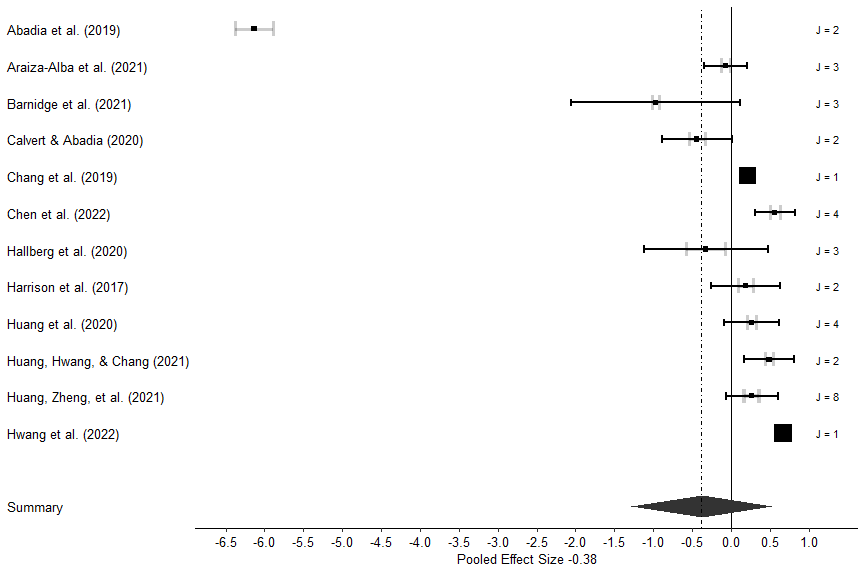
\includegraphics[width=1\textwidth,height=\textheight]{images/3lmaforest.png}

Absolutely beautiful plot right? I'll tell you what, I really love this plot. You can read about what the different items and colors mean in Fernández-Castilla et al.~(2020)\citep{fernández-castilla2020}. Remember, all of the code for the plots in this chapter are from their paper. But to quickly explain some major points, the black boxes represent the average effect size from the comparisons within each study, and the black lines are the study precision. The grey lines are the median precision of one effect size from each study. The size of the effect size box is representative of its weight in the analysis. J represents how many comparisons were analyzed from each study. I think that this is such a beautiful plot, one of my favorites in all of meta-analysis!

\hypertarget{caterpillar-plots}{%
\subsubsection{Caterpillar Plots}\label{caterpillar-plots}}

While forest plots are great, sometimes we want a different way to visualize our data. Caterpillar plots are an interesting way to visualize our data. Again, we borrow some code from Fernández-Castilla et al.~(2020)\citep{fernández-castilla2020}.

\hypertarget{all-comparisons}{%
\paragraph{All Comparisons}\label{all-comparisons}}

First, let's look at all comparisons in one plot:

\begin{Shaded}
\begin{Highlighting}[]
\NormalTok{Caterpillar}\OtherTok{\textless{}{-}}\ControlFlowTok{function}\NormalTok{(study, ES, out, var, se)\{ }
\NormalTok{  dataset}\OtherTok{\textless{}{-}}\FunctionTok{data.frame}\NormalTok{(study, ES, out, var, se)}
\NormalTok{  dataset}\SpecialCharTok{$}\NormalTok{cilb}\OtherTok{\textless{}{-}}\NormalTok{dataset}\SpecialCharTok{$}\NormalTok{ES}\SpecialCharTok{{-}}\NormalTok{(}\FloatTok{1.96}\SpecialCharTok{*}\NormalTok{dataset}\SpecialCharTok{$}\NormalTok{se)}
\NormalTok{  dataset}\SpecialCharTok{$}\NormalTok{ciub}\OtherTok{\textless{}{-}}\NormalTok{dataset}\SpecialCharTok{$}\NormalTok{ES}\SpecialCharTok{+}\NormalTok{(}\FloatTok{1.96}\SpecialCharTok{*}\NormalTok{dataset}\SpecialCharTok{$}\NormalTok{se)}
\NormalTok{meta\_abu }\OtherTok{\textless{}{-}} \FunctionTok{summary}\NormalTok{(}\FunctionTok{meta3}\NormalTok{(}\AttributeTok{y=}\NormalTok{ES, }\AttributeTok{v=}\NormalTok{var, }\AttributeTok{cluster=}\NormalTok{study, }\AttributeTok{data=}\NormalTok{dataset))}
\NormalTok{dataset}\OtherTok{\textless{}{-}}\NormalTok{dataset[}\FunctionTok{order}\NormalTok{(dataset}\SpecialCharTok{$}\NormalTok{ES),]}
\NormalTok{dataset}\SpecialCharTok{$}\NormalTok{id}\OtherTok{\textless{}{-}}\FunctionTok{c}\NormalTok{(}\FunctionTok{rep}\NormalTok{(}\DecValTok{1}\SpecialCharTok{:}\FunctionTok{length}\NormalTok{(dataset}\SpecialCharTok{$}\NormalTok{se)))}
\NormalTok{P\_combined}\OtherTok{\textless{}{-}}\FunctionTok{nrow}\NormalTok{(dataset)}\SpecialCharTok{+}\DecValTok{10}
\NormalTok{combined\_ES}\OtherTok{\textless{}{-}}\FunctionTok{data.frame}\NormalTok{(}\AttributeTok{ES=}\NormalTok{meta\_abu}\SpecialCharTok{$}\NormalTok{coefficients}\SpecialCharTok{$}\NormalTok{Estimate[}\DecValTok{1}\NormalTok{],}
                        \AttributeTok{cilb=}\NormalTok{meta\_abu}\SpecialCharTok{$}\NormalTok{coefficients}\SpecialCharTok{$}\NormalTok{lbound[}\DecValTok{1}\NormalTok{], }\AttributeTok{ciub=}\NormalTok{meta\_abu}\SpecialCharTok{$}\NormalTok{coefficients}\SpecialCharTok{$}\NormalTok{ubound[}\DecValTok{1}\NormalTok{],}
                        \AttributeTok{id=}\NormalTok{P\_combined)}


\NormalTok{minimum}\OtherTok{\textless{}{-}}\FunctionTok{min}\NormalTok{(dataset}\SpecialCharTok{$}\NormalTok{cilb)}
\NormalTok{maximum}\OtherTok{\textless{}{-}}\FunctionTok{max}\NormalTok{(dataset}\SpecialCharTok{$}\NormalTok{ciub)}
\NormalTok{lim\_minimum}\OtherTok{\textless{}{-}}\NormalTok{minimum}\FloatTok{{-}0.10}
\NormalTok{lim\_maximum}\OtherTok{\textless{}{-}}\NormalTok{maximum}\FloatTok{+0.10}
\NormalTok{r\_lim\_minimum}\OtherTok{\textless{}{-}}\FunctionTok{round}\NormalTok{(lim\_minimum, }\AttributeTok{digits=}\DecValTok{0}\NormalTok{)}
\NormalTok{r\_lim\_maximum}\OtherTok{\textless{}{-}}\FunctionTok{round}\NormalTok{(lim\_maximum, }\AttributeTok{digits=}\DecValTok{0}\NormalTok{)}
\NormalTok{abs\_r\_lim\_minimum}\OtherTok{\textless{}{-}}\FunctionTok{abs}\NormalTok{(r\_lim\_minimum)}
\NormalTok{abs\_r\_lim\_maximum}\OtherTok{\textless{}{-}}\FunctionTok{abs}\NormalTok{(r\_lim\_maximum)}
\NormalTok{dec\_min}\OtherTok{\textless{}{-}}\FunctionTok{round}\NormalTok{(}\FunctionTok{abs}\NormalTok{((lim\_minimum}\SpecialCharTok{{-}}\NormalTok{r\_lim\_minimum)}\SpecialCharTok{*}\DecValTok{100}\NormalTok{), }\AttributeTok{digits=}\DecValTok{0}\NormalTok{)}
\NormalTok{dec\_max}\OtherTok{\textless{}{-}}\FunctionTok{round}\NormalTok{(}\FunctionTok{abs}\NormalTok{((lim\_maximum}\SpecialCharTok{{-}}\NormalTok{r\_lim\_maximum)}\SpecialCharTok{*}\DecValTok{100}\NormalTok{), }\AttributeTok{digits=}\DecValTok{0}\NormalTok{)}

\ControlFlowTok{if}\NormalTok{ (dec\_min }\SpecialCharTok{\textless{}} \DecValTok{25}\NormalTok{) \{}
\NormalTok{  c}\OtherTok{=}\DecValTok{25}\SpecialCharTok{/}\DecValTok{100}
\NormalTok{\} }\ControlFlowTok{else} \ControlFlowTok{if}\NormalTok{ (dec\_min}\SpecialCharTok{\textgreater{}}\DecValTok{25} \SpecialCharTok{\&}\NormalTok{ dec\_min}\SpecialCharTok{\textless{}}\DecValTok{50}\NormalTok{) \{}
\NormalTok{  c}\OtherTok{=}\DecValTok{50}\SpecialCharTok{/}\DecValTok{100}
\NormalTok{\} }\ControlFlowTok{else} \ControlFlowTok{if}\NormalTok{ (dec\_min}\SpecialCharTok{\textgreater{}}\DecValTok{50} \SpecialCharTok{\&}\NormalTok{ dec\_min}\SpecialCharTok{\textless{}}\DecValTok{75}\NormalTok{) \{}
\NormalTok{  c}\OtherTok{=}\DecValTok{75}\SpecialCharTok{/}\DecValTok{100}
\NormalTok{\} }\ControlFlowTok{else}\NormalTok{ \{}
\NormalTok{  c}\OtherTok{=}\NormalTok{abs\_r\_lim\_minimum}\SpecialCharTok{+}\DecValTok{1}
\NormalTok{\}}

\ControlFlowTok{if}\NormalTok{ (dec\_max }\SpecialCharTok{\textless{}} \DecValTok{25}\NormalTok{) \{}
\NormalTok{  d}\OtherTok{=}\DecValTok{25}\SpecialCharTok{/}\DecValTok{100}
\NormalTok{\} }\ControlFlowTok{else} \ControlFlowTok{if}\NormalTok{ (dec\_max}\SpecialCharTok{\textgreater{}}\DecValTok{25} \SpecialCharTok{\&}\NormalTok{ dec\_max}\SpecialCharTok{\textless{}}\DecValTok{50}\NormalTok{) \{}
\NormalTok{  d}\OtherTok{=}\DecValTok{50}\SpecialCharTok{/}\DecValTok{100}
\NormalTok{\} }\ControlFlowTok{else} \ControlFlowTok{if}\NormalTok{ (dec\_max}\SpecialCharTok{\textgreater{}}\DecValTok{50} \SpecialCharTok{\&}\NormalTok{ dec\_max}\SpecialCharTok{\textless{}}\DecValTok{75}\NormalTok{) \{}
\NormalTok{  d}\OtherTok{=}\DecValTok{75}\SpecialCharTok{/}\DecValTok{100}
\NormalTok{\} }\ControlFlowTok{else}\NormalTok{ \{}
\NormalTok{  d}\OtherTok{=}\NormalTok{abs\_r\_lim\_maximum}\SpecialCharTok{+}\DecValTok{1}
\NormalTok{\}}

\NormalTok{lim\_minimum}\OtherTok{\textless{}{-}}\NormalTok{r\_lim\_minimum}\SpecialCharTok{{-}}\NormalTok{c}
\NormalTok{lim\_maximum}\OtherTok{\textless{}{-}}\NormalTok{r\_lim\_maximum}\SpecialCharTok{+}\NormalTok{d}

\NormalTok{Axis\_ES }\OtherTok{\textless{}{-}} \FunctionTok{seq}\NormalTok{(lim\_minimum, lim\_maximum, }\AttributeTok{by=}\DecValTok{2}\NormalTok{)}
\CommentTok{\#Axis\_ES\textless{}{-} c(Axis\_ES,0)}
\NormalTok{Axis\_ES}\OtherTok{\textless{}{-}}\NormalTok{Axis\_ES[}\FunctionTok{order}\NormalTok{(Axis\_ES)]}

\NormalTok{p }\OtherTok{\textless{}{-}} \FunctionTok{ggplot}\NormalTok{()}\SpecialCharTok{+}
  \FunctionTok{geom\_point}\NormalTok{(}\AttributeTok{data=}\NormalTok{dataset, }\FunctionTok{aes}\NormalTok{(}\AttributeTok{y=}\NormalTok{id, }\AttributeTok{x=}\NormalTok{ES),}\AttributeTok{colour =} \StringTok{"black"}\NormalTok{)}\SpecialCharTok{+}
  \FunctionTok{geom\_errorbarh}\NormalTok{(}\AttributeTok{data=}\NormalTok{dataset, }\FunctionTok{aes}\NormalTok{(}\AttributeTok{y=}\NormalTok{id, }\AttributeTok{x=}\NormalTok{ES, }\AttributeTok{xmin =}\NormalTok{ cilb, }\AttributeTok{xmax =}\NormalTok{ ciub),}\AttributeTok{size=}\DecValTok{1}\NormalTok{,  }\AttributeTok{height=}\NormalTok{.}\DecValTok{2}\NormalTok{)}\SpecialCharTok{+}
  \FunctionTok{scale\_x\_continuous}\NormalTok{(}\AttributeTok{limits=}\FunctionTok{c}\NormalTok{(lim\_minimum,lim\_maximum),}\AttributeTok{breaks=}\NormalTok{Axis\_ES)}\SpecialCharTok{+} 
  \FunctionTok{geom\_vline}\NormalTok{(}\AttributeTok{xintercept=}\DecValTok{0}\NormalTok{,}\AttributeTok{size=}\FloatTok{1.2}\NormalTok{, }\AttributeTok{alpha=}\FloatTok{0.7}\NormalTok{,}\AttributeTok{colour=}\StringTok{"\#EF3B2C"}\NormalTok{, }\AttributeTok{linetype=}\StringTok{"twodash"}\NormalTok{)}
\NormalTok{p}\OtherTok{\textless{}{-}}\NormalTok{p}\SpecialCharTok{+}
  \FunctionTok{geom\_point}\NormalTok{(}\AttributeTok{data=}\NormalTok{combined\_ES, }\FunctionTok{aes}\NormalTok{(}\AttributeTok{y=}\NormalTok{id, }\AttributeTok{x=}\NormalTok{ES), }\AttributeTok{colour =} \StringTok{"red"}\NormalTok{, }\AttributeTok{size=}\DecValTok{2}\NormalTok{)}\SpecialCharTok{+}
  \FunctionTok{geom\_errorbarh}\NormalTok{(}\AttributeTok{data=}\NormalTok{combined\_ES, }\FunctionTok{aes}\NormalTok{(}\AttributeTok{y=}\NormalTok{id, }\AttributeTok{x=}\NormalTok{ES, }\AttributeTok{xmin =}\NormalTok{ cilb, }\AttributeTok{xmax =}\NormalTok{ ciub), }\AttributeTok{colour=}\StringTok{"red"}\NormalTok{, }\AttributeTok{size=}\DecValTok{1}\NormalTok{,  }\AttributeTok{height=}\NormalTok{.}\DecValTok{2}\NormalTok{)}\SpecialCharTok{+}
  \FunctionTok{coord\_flip}\NormalTok{()}\SpecialCharTok{+}
  \FunctionTok{theme}\NormalTok{( }\AttributeTok{axis.line=}\FunctionTok{element\_blank}\NormalTok{(), }\AttributeTok{panel.grid.major =} \FunctionTok{element\_blank}\NormalTok{(), }\AttributeTok{panel.grid.minor =} \FunctionTok{element\_blank}\NormalTok{(),}
         \AttributeTok{legend.position=}\StringTok{"none"}\NormalTok{,}\AttributeTok{panel.background =} \FunctionTok{element\_blank}\NormalTok{(), }\AttributeTok{axis.line.x =} \FunctionTok{element\_blank}\NormalTok{(), }\AttributeTok{axis.line.y =} \FunctionTok{element\_line}\NormalTok{(}\AttributeTok{colour =} \StringTok{"black"}\NormalTok{),}
         \AttributeTok{axis.title.x=}\FunctionTok{element\_blank}\NormalTok{(), }\AttributeTok{axis.title.y=}\FunctionTok{element\_text}\NormalTok{(}\AttributeTok{size=}\DecValTok{14}\NormalTok{), }\AttributeTok{axis.text.y =} \FunctionTok{element\_text}\NormalTok{(}\AttributeTok{size=}\DecValTok{12}\NormalTok{, }\AttributeTok{color=}\StringTok{"black"}\NormalTok{), }\AttributeTok{axis.text.x =} \FunctionTok{element\_blank}\NormalTok{(), }\AttributeTok{axis.ticks =} \FunctionTok{element\_blank}\NormalTok{())}\SpecialCharTok{+}
  \FunctionTok{xlab}\NormalTok{(}\StringTok{"Effect sizes"}\NormalTok{)}

\FunctionTok{print}\NormalTok{(p)}

\NormalTok{\}}
\FunctionTok{Caterpillar}\NormalTok{(study, ES, out, var, se)}
\end{Highlighting}
\end{Shaded}

\emph{What's this code doing?}

This code creates a caterpillar plot of all comparisons in the analysis.

That should create a plot like this:

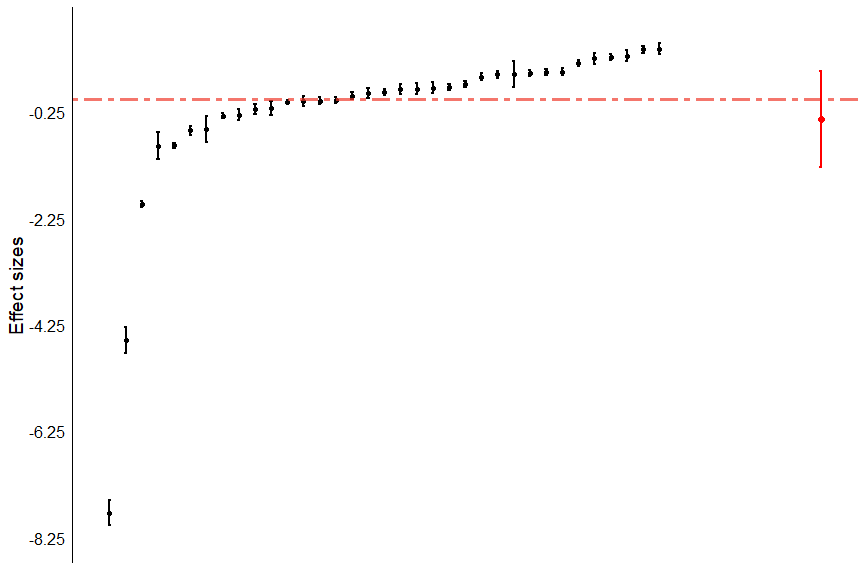
\includegraphics[width=1\textwidth,height=\textheight]{images/caterpillar_all.png}

As you can see, all 35 comparisons are included in this plot, listed from smallest (left) to largest (right). The red line is our overall meta-analytic effect size.

\hypertarget{study-level-plot}{%
\paragraph{Study-Level Plot}\label{study-level-plot}}

If you prefer a plot of study level results, similar to the forest plot, we can use this code, again from Fernández-Castilla et al.~(2020)\citep{fernández-castilla2020}:

\begin{Shaded}
\begin{Highlighting}[]

\NormalTok{caterpillar\_studies}\OtherTok{\textless{}{-}}\ControlFlowTok{function}\NormalTok{(study, ES, out, var, se)\{}
\NormalTok{dataset}\OtherTok{\textless{}{-}}\FunctionTok{data.frame}\NormalTok{(study, ES, out, var, se)}
\NormalTok{  meta\_abu }\OtherTok{\textless{}{-}} \FunctionTok{summary}\NormalTok{(}\FunctionTok{meta3}\NormalTok{(}\AttributeTok{y=}\NormalTok{ES, }\AttributeTok{v=}\NormalTok{var, }\AttributeTok{cluster=}\NormalTok{study, }\AttributeTok{data=}\NormalTok{dataset))}
\NormalTok{  row }\OtherTok{=} \DecValTok{1}
\NormalTok{  nrow}\OtherTok{=}\FunctionTok{max}\NormalTok{(dataset}\SpecialCharTok{$}\NormalTok{study)}
\NormalTok{  studyn}\OtherTok{=}\FunctionTok{max}\NormalTok{(dataset}\SpecialCharTok{$}\NormalTok{study)}
\NormalTok{  studyinfo }\OtherTok{=} \FunctionTok{data.frame}\NormalTok{(}\AttributeTok{Study =} \FunctionTok{numeric}\NormalTok{(nrow),}
                         \AttributeTok{ES=} \FunctionTok{numeric}\NormalTok{(nrow),}
                         \AttributeTok{SE=} \FunctionTok{numeric}\NormalTok{(nrow),}
                         \AttributeTok{cilb=} \FunctionTok{numeric}\NormalTok{(nrow),}
                         \AttributeTok{ciub=} \FunctionTok{numeric}\NormalTok{(nrow),}
                         \AttributeTok{S\_cilb=}\FunctionTok{numeric}\NormalTok{(nrow),}
                         \AttributeTok{S\_ciub=}\FunctionTok{numeric}\NormalTok{(nrow))}
\NormalTok{  Study1 }\OtherTok{=}\FunctionTok{c}\NormalTok{()}
\NormalTok{  Study2 }\OtherTok{=}\FunctionTok{c}\NormalTok{()}
  
  \ControlFlowTok{for}\NormalTok{ (i }\ControlFlowTok{in} \DecValTok{1}\SpecialCharTok{:}\FunctionTok{max}\NormalTok{(dataset}\SpecialCharTok{$}\NormalTok{study))\{}
\NormalTok{    data}\OtherTok{\textless{}{-}}\FunctionTok{subset}\NormalTok{(dataset, study}\SpecialCharTok{==}\NormalTok{i)}
\NormalTok{    uni}\OtherTok{=}\FunctionTok{nrow}\NormalTok{(data)}
    \ControlFlowTok{if}\NormalTok{ (uni}\SpecialCharTok{==}\DecValTok{1}\NormalTok{) \{}
\NormalTok{      studyinfo}\SpecialCharTok{$}\NormalTok{ES[row]}\OtherTok{\textless{}{-}}\NormalTok{data}\SpecialCharTok{$}\NormalTok{ES}
\NormalTok{      studyinfo}\SpecialCharTok{$}\NormalTok{SE[row]}\OtherTok{\textless{}{-}}\NormalTok{data}\SpecialCharTok{$}\NormalTok{se}
\NormalTok{      studyinfo}\SpecialCharTok{$}\NormalTok{cilb[row]}\OtherTok{\textless{}{-}}\NormalTok{(data}\SpecialCharTok{$}\NormalTok{ES}\SpecialCharTok{{-}}\NormalTok{(data}\SpecialCharTok{$}\NormalTok{se}\SpecialCharTok{*}\FloatTok{1.96}\NormalTok{))}
\NormalTok{      studyinfo}\SpecialCharTok{$}\NormalTok{ciub[row]}\OtherTok{\textless{}{-}}\NormalTok{(data}\SpecialCharTok{$}\NormalTok{ES}\SpecialCharTok{+}\NormalTok{(data}\SpecialCharTok{$}\NormalTok{se}\SpecialCharTok{*}\FloatTok{1.96}\NormalTok{))}
\NormalTok{      studyinfo}\SpecialCharTok{$}\NormalTok{S\_cilb[row]}\OtherTok{\textless{}{-}}\NormalTok{(data}\SpecialCharTok{$}\NormalTok{ES}\SpecialCharTok{{-}}\NormalTok{(data}\SpecialCharTok{$}\NormalTok{se}\SpecialCharTok{*}\FloatTok{1.96}\NormalTok{))}
\NormalTok{      studyinfo}\SpecialCharTok{$}\NormalTok{S\_ciub[row]}\OtherTok{\textless{}{-}}\NormalTok{(data}\SpecialCharTok{$}\NormalTok{ES}\SpecialCharTok{+}\NormalTok{(data}\SpecialCharTok{$}\NormalTok{se}\SpecialCharTok{*}\FloatTok{1.96}\NormalTok{)) }
\NormalTok{    \}}
    
    \ControlFlowTok{else}\NormalTok{ \{}
\NormalTok{    a}\OtherTok{\textless{}{-}}\FunctionTok{rma}\NormalTok{(}\AttributeTok{y=}\NormalTok{data}\SpecialCharTok{$}\NormalTok{ES, }\AttributeTok{vi=}\NormalTok{data}\SpecialCharTok{$}\NormalTok{var, }\AttributeTok{data=}\NormalTok{data, }\AttributeTok{method=}\StringTok{"REML"}\NormalTok{)}
\NormalTok{    studyinfo}\SpecialCharTok{$}\NormalTok{ES[row]}\OtherTok{\textless{}{-}}\NormalTok{a}\SpecialCharTok{$}\NormalTok{b}
\NormalTok{    studyinfo}\SpecialCharTok{$}\NormalTok{SE[row]}\OtherTok{\textless{}{-}}\NormalTok{a}\SpecialCharTok{$}\NormalTok{se}
\NormalTok{    studyinfo}\SpecialCharTok{$}\NormalTok{cilb[row]}\OtherTok{\textless{}{-}}\NormalTok{a}\SpecialCharTok{$}\NormalTok{ci.lb}
\NormalTok{    studyinfo}\SpecialCharTok{$}\NormalTok{ciub[row]}\OtherTok{\textless{}{-}}\NormalTok{a}\SpecialCharTok{$}\NormalTok{ci.ub}
\NormalTok{    studyinfo}\SpecialCharTok{$}\NormalTok{S\_cilb[row]}\OtherTok{\textless{}{-}}\NormalTok{a}\SpecialCharTok{$}\NormalTok{b }\SpecialCharTok{{-}} \FloatTok{1.96}\SpecialCharTok{*}\FunctionTok{median}\NormalTok{(data}\SpecialCharTok{$}\NormalTok{se)}
\NormalTok{    studyinfo}\SpecialCharTok{$}\NormalTok{S\_ciub[row]}\OtherTok{\textless{}{-}}\NormalTok{a}\SpecialCharTok{$}\NormalTok{b }\SpecialCharTok{+} \FloatTok{1.96}\SpecialCharTok{*}\FunctionTok{median}\NormalTok{(data}\SpecialCharTok{$}\NormalTok{se)}
\NormalTok{    \}}
\NormalTok{    studyinfo}\SpecialCharTok{$}\NormalTok{Study[row]}\OtherTok{\textless{}{-}}\FunctionTok{c}\NormalTok{(Study1,}\FunctionTok{paste}\NormalTok{(}\StringTok{"Study"}\NormalTok{,i))}
\NormalTok{    row }\OtherTok{=}\NormalTok{ row }\SpecialCharTok{+} \DecValTok{1}      
    
\NormalTok{  \}}
  
\NormalTok{  studyinfo}\OtherTok{\textless{}{-}}\NormalTok{ studyinfo[}\FunctionTok{order}\NormalTok{(studyinfo}\SpecialCharTok{$}\NormalTok{ES),]}
\NormalTok{  studyinfo}\SpecialCharTok{$}\NormalTok{id}\OtherTok{\textless{}{-}}\FunctionTok{c}\NormalTok{(}\FunctionTok{rep}\NormalTok{(}\DecValTok{1}\SpecialCharTok{:}\FunctionTok{length}\NormalTok{(studyinfo}\SpecialCharTok{$}\NormalTok{ES)))}
  
\NormalTok{  P\_combined}\OtherTok{\textless{}{-}}\FunctionTok{nrow}\NormalTok{(studyinfo)}\SpecialCharTok{+}\DecValTok{2}
\NormalTok{  combined\_ES}\OtherTok{\textless{}{-}}\FunctionTok{data.frame}\NormalTok{(}\AttributeTok{ES=}\NormalTok{meta\_abu}\SpecialCharTok{$}\NormalTok{coefficients}\SpecialCharTok{$}\NormalTok{Estimate[}\DecValTok{1}\NormalTok{],}
                          \AttributeTok{cilb=}\NormalTok{meta\_abu}\SpecialCharTok{$}\NormalTok{coefficients}\SpecialCharTok{$}\NormalTok{lbound[}\DecValTok{1}\NormalTok{], }\AttributeTok{ciub=}\NormalTok{meta\_abu}\SpecialCharTok{$}\NormalTok{coefficients}\SpecialCharTok{$}\NormalTok{ubound[}\DecValTok{1}\NormalTok{],}
                          \AttributeTok{id=}\NormalTok{P\_combined)}
  
  
\NormalTok{  minimum}\OtherTok{\textless{}{-}}\FunctionTok{min}\NormalTok{(studyinfo}\SpecialCharTok{$}\NormalTok{S\_cilb)}
\NormalTok{  maximum}\OtherTok{\textless{}{-}}\FunctionTok{max}\NormalTok{(studyinfo}\SpecialCharTok{$}\NormalTok{S\_ciub)}
\NormalTok{  lim\_minimum}\OtherTok{\textless{}{-}}\NormalTok{minimum}\FloatTok{{-}0.10}
\NormalTok{  lim\_maximum}\OtherTok{\textless{}{-}}\NormalTok{maximum}\FloatTok{+0.10}
\NormalTok{  r\_lim\_minimum}\OtherTok{\textless{}{-}}\FunctionTok{round}\NormalTok{(lim\_minimum, }\AttributeTok{digits=}\DecValTok{0}\NormalTok{)}
\NormalTok{  r\_lim\_maximum}\OtherTok{\textless{}{-}}\FunctionTok{round}\NormalTok{(lim\_maximum, }\AttributeTok{digits=}\DecValTok{0}\NormalTok{)}
\NormalTok{  abs\_r\_lim\_minimum}\OtherTok{\textless{}{-}}\FunctionTok{abs}\NormalTok{(r\_lim\_minimum)}
\NormalTok{  abs\_r\_lim\_maximum}\OtherTok{\textless{}{-}}\FunctionTok{abs}\NormalTok{(r\_lim\_maximum)}
\NormalTok{  dec\_min}\OtherTok{\textless{}{-}}\FunctionTok{round}\NormalTok{(}\FunctionTok{abs}\NormalTok{((lim\_minimum}\SpecialCharTok{{-}}\NormalTok{r\_lim\_minimum)}\SpecialCharTok{*}\DecValTok{100}\NormalTok{), }\AttributeTok{digits=}\DecValTok{0}\NormalTok{)}
\NormalTok{  dec\_max}\OtherTok{\textless{}{-}}\FunctionTok{round}\NormalTok{(}\FunctionTok{abs}\NormalTok{((lim\_maximum}\SpecialCharTok{{-}}\NormalTok{r\_lim\_maximum)}\SpecialCharTok{*}\DecValTok{100}\NormalTok{), }\AttributeTok{digits=}\DecValTok{0}\NormalTok{)}
  
  \ControlFlowTok{if}\NormalTok{ (dec\_min }\SpecialCharTok{\textless{}} \DecValTok{25}\NormalTok{) \{}
\NormalTok{    c}\OtherTok{=}\DecValTok{25}\SpecialCharTok{/}\DecValTok{100}
\NormalTok{  \} }\ControlFlowTok{else} \ControlFlowTok{if}\NormalTok{ (dec\_min}\SpecialCharTok{\textgreater{}}\DecValTok{25} \SpecialCharTok{\&}\NormalTok{ dec\_min}\SpecialCharTok{\textless{}}\DecValTok{50}\NormalTok{) \{}
\NormalTok{    c}\OtherTok{=}\DecValTok{50}\SpecialCharTok{/}\DecValTok{100}
\NormalTok{  \} }\ControlFlowTok{else} \ControlFlowTok{if}\NormalTok{ (dec\_min}\SpecialCharTok{\textgreater{}}\DecValTok{50} \SpecialCharTok{\&}\NormalTok{ dec\_min}\SpecialCharTok{\textless{}}\DecValTok{75}\NormalTok{) \{}
\NormalTok{    c}\OtherTok{=}\DecValTok{75}\SpecialCharTok{/}\DecValTok{100}
\NormalTok{  \} }\ControlFlowTok{else}\NormalTok{ \{}
\NormalTok{    c}\OtherTok{=}\NormalTok{abs\_r\_lim\_minimum}\SpecialCharTok{+}\DecValTok{1}
\NormalTok{  \}}
  
  \ControlFlowTok{if}\NormalTok{ (dec\_max }\SpecialCharTok{\textless{}} \DecValTok{25}\NormalTok{) \{}
\NormalTok{    d}\OtherTok{=}\DecValTok{25}\SpecialCharTok{/}\DecValTok{100}
\NormalTok{  \} }\ControlFlowTok{else} \ControlFlowTok{if}\NormalTok{ (dec\_max}\SpecialCharTok{\textgreater{}}\DecValTok{25} \SpecialCharTok{\&}\NormalTok{ dec\_max}\SpecialCharTok{\textless{}}\DecValTok{50}\NormalTok{) \{}
\NormalTok{    d}\OtherTok{=}\DecValTok{50}\SpecialCharTok{/}\DecValTok{100}
\NormalTok{  \} }\ControlFlowTok{else} \ControlFlowTok{if}\NormalTok{ (dec\_max}\SpecialCharTok{\textgreater{}}\DecValTok{50} \SpecialCharTok{\&}\NormalTok{ dec\_max}\SpecialCharTok{\textless{}}\DecValTok{75}\NormalTok{) \{}
\NormalTok{    d}\OtherTok{=}\DecValTok{75}\SpecialCharTok{/}\DecValTok{100}
\NormalTok{  \} }\ControlFlowTok{else}\NormalTok{ \{}
\NormalTok{    d}\OtherTok{=}\NormalTok{abs\_r\_lim\_maximum}\SpecialCharTok{+}\DecValTok{1}
\NormalTok{  \}}
  
\NormalTok{  lim\_minimum}\OtherTok{\textless{}{-}}\NormalTok{r\_lim\_minimum}\SpecialCharTok{{-}}\NormalTok{c}
\NormalTok{  lim\_maximum}\OtherTok{\textless{}{-}}\NormalTok{r\_lim\_maximum}\SpecialCharTok{+}\NormalTok{d}
  
\NormalTok{  Axis\_ES }\OtherTok{\textless{}{-}} \FunctionTok{seq}\NormalTok{(lim\_minimum, lim\_maximum, }\AttributeTok{by=}\FloatTok{0.50}\NormalTok{)}
\NormalTok{  Axis\_ES}\OtherTok{\textless{}{-}} \FunctionTok{c}\NormalTok{(Axis\_ES,}\DecValTok{0}\NormalTok{)}
\NormalTok{  Axis\_ES}\OtherTok{\textless{}{-}}\NormalTok{Axis\_ES[}\FunctionTok{order}\NormalTok{(Axis\_ES)]}
  
  
\NormalTok{  r }\OtherTok{\textless{}{-}} \FunctionTok{ggplot}\NormalTok{()}\SpecialCharTok{+}
    \FunctionTok{geom\_point}\NormalTok{(}\AttributeTok{data=}\NormalTok{studyinfo, }\FunctionTok{aes}\NormalTok{(}\AttributeTok{y=}\NormalTok{id, }\AttributeTok{x=}\NormalTok{ES),}\AttributeTok{colour =} \StringTok{"black"}\NormalTok{)}\SpecialCharTok{+}
    \FunctionTok{geom\_errorbarh}\NormalTok{(}\AttributeTok{data=}\NormalTok{studyinfo, }\FunctionTok{aes}\NormalTok{(}\AttributeTok{y=}\NormalTok{id, }\AttributeTok{x=}\NormalTok{ES, }\AttributeTok{xmin =}\NormalTok{ cilb, }\AttributeTok{xmax =}\NormalTok{ ciub),  }\AttributeTok{size=}\DecValTok{1}\NormalTok{, }\AttributeTok{height=}\NormalTok{.}\DecValTok{2}\NormalTok{)}\SpecialCharTok{+}
    \FunctionTok{scale\_x\_continuous}\NormalTok{(}\AttributeTok{limits=}\FunctionTok{c}\NormalTok{(lim\_minimum,lim\_maximum),}\AttributeTok{breaks=}\NormalTok{Axis\_ES)}\SpecialCharTok{+} 
    \FunctionTok{geom\_vline}\NormalTok{(}\AttributeTok{xintercept=}\DecValTok{0}\NormalTok{,}\AttributeTok{size=}\FloatTok{1.2}\NormalTok{, }\AttributeTok{alpha=}\FloatTok{0.7}\NormalTok{,}\AttributeTok{colour=}\StringTok{"\#EF3B2C"}\NormalTok{, }\AttributeTok{linetype=}\StringTok{"twodash"}\NormalTok{)}
  
\NormalTok{  r}\OtherTok{\textless{}{-}}\NormalTok{r }\SpecialCharTok{+} \FunctionTok{geom\_point}\NormalTok{(}\AttributeTok{data=}\NormalTok{studyinfo, }\FunctionTok{aes}\NormalTok{(}\AttributeTok{y=}\NormalTok{id, }\AttributeTok{x=}\NormalTok{ES),}\AttributeTok{colour =} \StringTok{"black"}\NormalTok{)}\SpecialCharTok{+}
    \FunctionTok{geom\_errorbarh}\NormalTok{(}\AttributeTok{data=}\NormalTok{studyinfo, }\FunctionTok{aes}\NormalTok{(}\AttributeTok{y=}\NormalTok{id, }\AttributeTok{x=}\NormalTok{ES, }\AttributeTok{xmin =}\NormalTok{ S\_cilb, }\AttributeTok{xmax =}\NormalTok{  S\_ciub),}\AttributeTok{width=}\NormalTok{.}\DecValTok{2}\NormalTok{,  }\AttributeTok{height=}\NormalTok{.}\DecValTok{2}\NormalTok{, }\AttributeTok{alpha=}\NormalTok{.}\DecValTok{5}\NormalTok{)}\SpecialCharTok{+}
    \FunctionTok{geom\_point}\NormalTok{(}\AttributeTok{data=}\NormalTok{combined\_ES, }\FunctionTok{aes}\NormalTok{(}\AttributeTok{y=}\NormalTok{id, }\AttributeTok{x=}\NormalTok{ES),}\AttributeTok{colour =} \StringTok{"red"}\NormalTok{, }\AttributeTok{size=}\DecValTok{2}\NormalTok{)}\SpecialCharTok{+}
    \FunctionTok{geom\_errorbarh}\NormalTok{(}\AttributeTok{data=}\NormalTok{combined\_ES, }\FunctionTok{aes}\NormalTok{(}\AttributeTok{y=}\NormalTok{id, }\AttributeTok{x=}\NormalTok{ES, }\AttributeTok{xmin =}\NormalTok{ cilb, }\AttributeTok{xmax =}\NormalTok{ciub),}\AttributeTok{height=}\NormalTok{.}\DecValTok{2}\NormalTok{, }\AttributeTok{colour =} \StringTok{"red"}\NormalTok{)}\SpecialCharTok{+}
    \FunctionTok{coord\_flip}\NormalTok{()}\SpecialCharTok{+}
    \FunctionTok{theme}\NormalTok{(}\AttributeTok{axis.line=}\FunctionTok{element\_blank}\NormalTok{(), }\AttributeTok{panel.grid.major =} \FunctionTok{element\_blank}\NormalTok{(), }\AttributeTok{panel.grid.minor =} \FunctionTok{element\_blank}\NormalTok{(),}
          \AttributeTok{legend.position=}\StringTok{"none"}\NormalTok{,}\AttributeTok{panel.background =} \FunctionTok{element\_blank}\NormalTok{(), }\AttributeTok{axis.line.x =} \FunctionTok{element\_blank}\NormalTok{(), }\AttributeTok{axis.line.y =} \FunctionTok{element\_line}\NormalTok{(}\AttributeTok{colour =} \StringTok{"black"}\NormalTok{),}
          \AttributeTok{axis.title.x=}\FunctionTok{element\_blank}\NormalTok{(), }\AttributeTok{axis.title.y=}\FunctionTok{element\_text}\NormalTok{(}\AttributeTok{size=}\DecValTok{14}\NormalTok{), }\AttributeTok{axis.text.y =} \FunctionTok{element\_text}\NormalTok{(}\AttributeTok{size=}\DecValTok{12}\NormalTok{, }\AttributeTok{color=}\StringTok{"black"}\NormalTok{), }\AttributeTok{axis.text.x =} \FunctionTok{element\_blank}\NormalTok{(), }\AttributeTok{axis.ticks =} \FunctionTok{element\_blank}\NormalTok{())}\SpecialCharTok{+}
    \FunctionTok{xlab}\NormalTok{(}\StringTok{"Meta{-}analytic study means"}\NormalTok{)}
  
 \FunctionTok{print}\NormalTok{(r)}
\NormalTok{\}}

\FunctionTok{caterpillar\_studies}\NormalTok{(study, ES, out, var, se)}
\end{Highlighting}
\end{Shaded}

\emph{What's this code doing?}

This code creates a caterpillar plot of study level effects rather than the comparison level.

That should produce this plot:

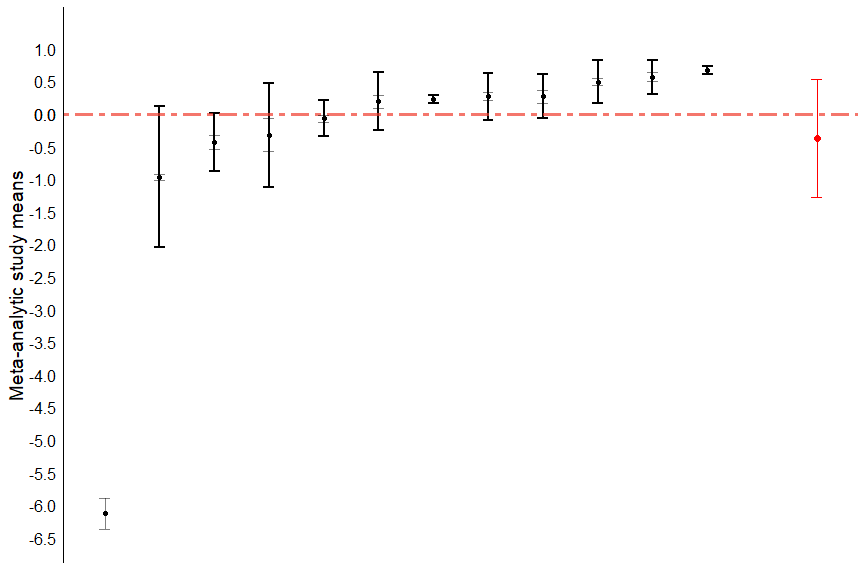
\includegraphics[width=1\textwidth,height=\textheight]{images/caterpillar_study.png}

Caterpillar plots are not, as of January 2024, very common in the educational literature. However, I see value in including the visualization in my publications.

\hypertarget{publication-bias-1}{%
\subsection{Publication Bias}\label{publication-bias-1}}

Oh we're not done yet, we haven't even talked about publication bias yet! Publication bias is more difficult to examine in three-level models than conventional meta-analysis models. Furthermore, the tests we have for conventional models often don't function well in three-level applications (Rodgers \& Pustejovsky, 2021)\citep{rodgers2021}. Instead, we can look at funnel plots to examine them for asymmetry.

\hypertarget{funnel-plots}{%
\subsubsection{Funnel Plots}\label{funnel-plots}}

Again, we're going to borrow the methods and adapt the code from Fernández-Castilla et al.~(2020)\citep{fernández-castilla2020}.

First we'll create a funnel plot of all effect sizes and check it for asymmetry.

\begin{Shaded}
\begin{Highlighting}[]
\NormalTok{three\_funnel}\OtherTok{\textless{}{-}}\ControlFlowTok{function}\NormalTok{(study, ES, out, var, se)\{}
  
\NormalTok{dataset}\OtherTok{\textless{}{-}}\FunctionTok{data.frame}\NormalTok{(study, ES, out, var, se)}
\NormalTok{contour.points}\OtherTok{=}\DecValTok{200}
\NormalTok{meta\_abu }\OtherTok{\textless{}{-}} \FunctionTok{summary}\NormalTok{(}\FunctionTok{meta3}\NormalTok{(}\AttributeTok{y=}\NormalTok{ES, }\AttributeTok{v=}\NormalTok{var, }\AttributeTok{cluster=}\NormalTok{study, }\AttributeTok{data=}\NormalTok{dataset))}
\NormalTok{estimate}\OtherTok{\textless{}{-}}\NormalTok{meta\_abu}\SpecialCharTok{$}\NormalTok{coefficients}\SpecialCharTok{$}\NormalTok{Estimate[}\DecValTok{1}\NormalTok{]}
\NormalTok{tau}\OtherTok{\textless{}{-}}\NormalTok{meta\_abu}\SpecialCharTok{$}\NormalTok{coefficients}\SpecialCharTok{$}\NormalTok{Estimate[}\DecValTok{3}\NormalTok{]}
\NormalTok{out}\OtherTok{\textless{}{-}}\NormalTok{meta\_abu}\SpecialCharTok{$}\NormalTok{coefficients}\SpecialCharTok{$}\NormalTok{Estimate[}\DecValTok{2}\NormalTok{]}

\NormalTok{maxse}\OtherTok{\textless{}{-}}\FunctionTok{max}\NormalTok{(dataset}\SpecialCharTok{$}\NormalTok{se)}
\NormalTok{ylim}\OtherTok{\textless{}{-}}\FunctionTok{c}\NormalTok{(}\DecValTok{0}\NormalTok{, maxse)}
\NormalTok{csize }\OtherTok{\textless{}{-}} \FunctionTok{seq}\NormalTok{(ylim[}\DecValTok{1}\NormalTok{], ylim[}\DecValTok{2}\NormalTok{], }\AttributeTok{length.out =}\NormalTok{ contour.points)}
\NormalTok{csize[csize }\SpecialCharTok{\textless{}=} \DecValTok{0}\NormalTok{] }\OtherTok{\textless{}{-}} \FloatTok{1e{-}07} \SpecialCharTok{*} \FunctionTok{min}\NormalTok{(dataset}\SpecialCharTok{$}\NormalTok{se)}
\NormalTok{csize}

\NormalTok{CI\_Lim}\OtherTok{\textless{}{-}}\FunctionTok{matrix}\NormalTok{(}\DecValTok{0}\NormalTok{, }\AttributeTok{nrow=}\FunctionTok{length}\NormalTok{(csize), }\AttributeTok{ncol=}\DecValTok{2}\NormalTok{)}
\FunctionTok{colnames}\NormalTok{(CI\_Lim)}\OtherTok{\textless{}{-}}\FunctionTok{c}\NormalTok{(}\StringTok{"lb\_total"}\NormalTok{, }\StringTok{"ub\_total"}\NormalTok{)}

\ControlFlowTok{for}\NormalTok{ (i }\ControlFlowTok{in} \DecValTok{1}\SpecialCharTok{:}\FunctionTok{length}\NormalTok{(csize))\{}
\NormalTok{  CI\_Lim[i,}\DecValTok{1}\NormalTok{]}\OtherTok{\textless{}{-}}\NormalTok{estimate}\FloatTok{{-}1.96}\SpecialCharTok{*}\FunctionTok{sqrt}\NormalTok{((csize[i]}\SpecialCharTok{\^{}}\DecValTok{2}\NormalTok{)}\SpecialCharTok{+}\NormalTok{tau}\SpecialCharTok{+}\NormalTok{out) }\CommentTok{\#add 1.96*}
\NormalTok{  CI\_Lim[i,}\DecValTok{2}\NormalTok{]}\OtherTok{\textless{}{-}}\NormalTok{estimate}\FloatTok{+1.96}\SpecialCharTok{*}\FunctionTok{sqrt}\NormalTok{((csize[i]}\SpecialCharTok{\^{}}\DecValTok{2}\NormalTok{)}\SpecialCharTok{+}\NormalTok{tau}\SpecialCharTok{+}\NormalTok{out)}
\NormalTok{\}}
\NormalTok{CI\_Lim}\OtherTok{\textless{}{-}}\FunctionTok{as.data.frame}\NormalTok{(CI\_Lim)}

\NormalTok{dataset}\SpecialCharTok{$}\NormalTok{study}\OtherTok{\textless{}{-}}\FunctionTok{as.character}\NormalTok{(dataset}\SpecialCharTok{$}\NormalTok{study)}
\NormalTok{dataset}\SpecialCharTok{$}\NormalTok{study }\OtherTok{\textless{}{-}} \FunctionTok{factor}\NormalTok{(dataset}\SpecialCharTok{$}\NormalTok{study)}
\NormalTok{geom.text.size }\OtherTok{=} \DecValTok{3}
\NormalTok{max\_SE}\OtherTok{\textless{}{-}}\FunctionTok{max}\NormalTok{(dataset}\SpecialCharTok{$}\NormalTok{se)}
\NormalTok{le}\OtherTok{\textless{}{-}}\FunctionTok{length}\NormalTok{(CI\_Lim[,}\DecValTok{1}\NormalTok{])}

\ControlFlowTok{if}\NormalTok{ ((CI\_Lim[le,}\DecValTok{1}\NormalTok{])}\SpecialCharTok{\textless{}} \DecValTok{0}\NormalTok{) \{}
\NormalTok{  minimum}\OtherTok{=}\FunctionTok{min}\NormalTok{(CI\_Lim[,}\DecValTok{1}\NormalTok{])}
\NormalTok{\} }\ControlFlowTok{else}\NormalTok{ \{}
\NormalTok{  minimum}\OtherTok{=}\FunctionTok{max}\NormalTok{(CI\_Lim[,}\DecValTok{1}\NormalTok{])}
\NormalTok{\} }

\ControlFlowTok{if}\NormalTok{ ((CI\_Lim[le,}\DecValTok{2}\NormalTok{]) }\SpecialCharTok{\textgreater{}} \DecValTok{0}\NormalTok{) \{}
\NormalTok{  maximum}\OtherTok{=}\FunctionTok{max}\NormalTok{(CI\_Lim[,}\DecValTok{2}\NormalTok{])}
\NormalTok{\} }\ControlFlowTok{else}\NormalTok{ \{}
\NormalTok{  maximum}\OtherTok{=}\FunctionTok{min}\NormalTok{(CI\_Lim[,}\DecValTok{2}\NormalTok{])}
\NormalTok{\} }


\NormalTok{lim\_minimum}\OtherTok{\textless{}{-}}\FunctionTok{floor}\NormalTok{(minimum}\FloatTok{{-}0.10}\NormalTok{)}
\NormalTok{lim\_maximum}\OtherTok{\textless{}{-}}\FunctionTok{ceiling}\NormalTok{(maximum}\FloatTok{+0.10}\NormalTok{)}
\NormalTok{Axis\_ES }\OtherTok{\textless{}{-}} \FunctionTok{seq}\NormalTok{(lim\_minimum, lim\_maximum, }\AttributeTok{by=}\DecValTok{1}\NormalTok{)}

\NormalTok{d }\OtherTok{\textless{}{-}} \FunctionTok{ggplot}\NormalTok{(}\AttributeTok{data=}\NormalTok{dataset, }\FunctionTok{aes}\NormalTok{(}\AttributeTok{x =}\NormalTok{ se, }\AttributeTok{y =}\NormalTok{ ES, }\FunctionTok{ylim}\NormalTok{(}\DecValTok{0}\NormalTok{,max\_SE)))}\SpecialCharTok{+}
  \FunctionTok{geom\_point}\NormalTok{()}\SpecialCharTok{+}
  \FunctionTok{xlab}\NormalTok{(}\StringTok{\textquotesingle{}Standard Error\textquotesingle{}}\NormalTok{)}\SpecialCharTok{+} 
  \FunctionTok{ylab}\NormalTok{(}\StringTok{\textquotesingle{}Effect size: g\textquotesingle{}}\NormalTok{)}\SpecialCharTok{+}
  \FunctionTok{geom\_hline}\NormalTok{(}\AttributeTok{yintercept=}\NormalTok{ estimate)}\SpecialCharTok{+}
  \FunctionTok{geom\_hline}\NormalTok{(}\AttributeTok{yintercept=} \DecValTok{0}\NormalTok{, }\AttributeTok{color=}\StringTok{\textquotesingle{}grey\textquotesingle{}}\NormalTok{)}\SpecialCharTok{+}
  \FunctionTok{scale\_x\_reverse}\NormalTok{()}\SpecialCharTok{+}
  \FunctionTok{scale\_y\_continuous}\NormalTok{(}\AttributeTok{breaks=}\NormalTok{Axis\_ES, }\AttributeTok{limits =}\FunctionTok{c}\NormalTok{(lim\_minimum,lim\_maximum))}\SpecialCharTok{+}
  \FunctionTok{coord\_flip}\NormalTok{()}\SpecialCharTok{+}
  \FunctionTok{theme}\NormalTok{(}\AttributeTok{panel.grid.major=}\FunctionTok{element\_blank}\NormalTok{(),}
        \AttributeTok{panel.grid.minor=}\FunctionTok{element\_blank}\NormalTok{(),}
        \AttributeTok{panel.border=}\FunctionTok{element\_blank}\NormalTok{(),}
        \AttributeTok{panel.background =} \FunctionTok{element\_blank}\NormalTok{(),}
        \AttributeTok{axis.line=}\FunctionTok{element\_line}\NormalTok{(),}
        \AttributeTok{axis.title =} \FunctionTok{element\_text}\NormalTok{(}\AttributeTok{size=}\DecValTok{14}\NormalTok{),}
        \AttributeTok{axis.text =} \FunctionTok{element\_text}\NormalTok{(}\AttributeTok{size=}\DecValTok{12}\NormalTok{, }\AttributeTok{color=}\StringTok{"black"}\NormalTok{),}
        \AttributeTok{text=}\FunctionTok{element\_text}\NormalTok{())}

\NormalTok{d }\OtherTok{\textless{}{-}}\NormalTok{ d }\SpecialCharTok{+} \FunctionTok{geom\_line}\NormalTok{(}\AttributeTok{data=}\NormalTok{CI\_Lim, }\FunctionTok{aes}\NormalTok{(}\AttributeTok{y=}\NormalTok{lb\_total, }\AttributeTok{x=}\NormalTok{csize), }\AttributeTok{colour=}\StringTok{"black"}\NormalTok{)}\SpecialCharTok{+}
  \FunctionTok{geom\_line}\NormalTok{(}\AttributeTok{data=}\NormalTok{CI\_Lim, }\FunctionTok{aes}\NormalTok{(}\AttributeTok{y=}\NormalTok{ub\_total, }\AttributeTok{x=}\NormalTok{csize), }\AttributeTok{colour=}\StringTok{"black"}\NormalTok{)}
\FunctionTok{print}\NormalTok{(d)}
\NormalTok{\}}

\FunctionTok{three\_funnel}\NormalTok{(study, ES, out, var, se)}
\end{Highlighting}
\end{Shaded}

\emph{What's this code doing?}

This code creates a funnel plot of all effect sizes.

When we run that code we'll see the following:

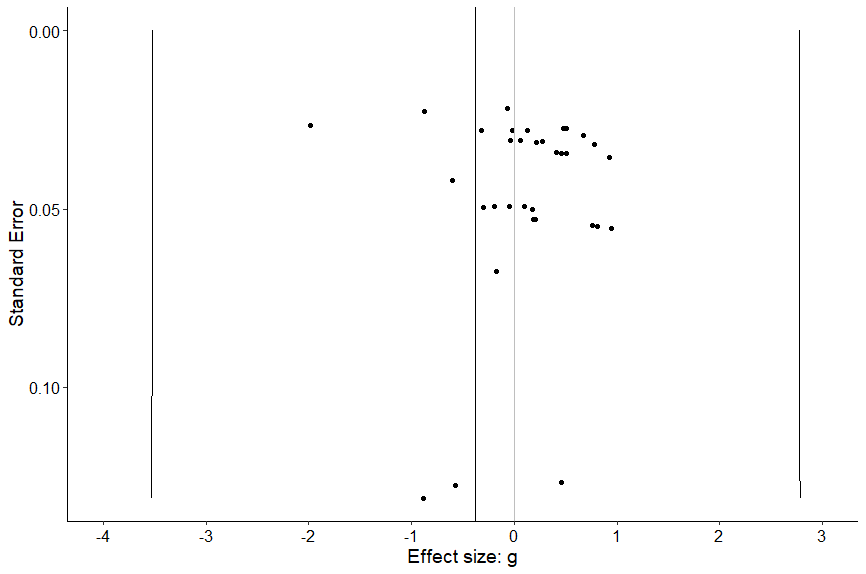
\includegraphics[width=1\textwidth,height=\textheight]{images/funnel_all.png}

The overall effect size is the grey vertical line to the left of zero. We want to see symmetry around that line, vertically and horizontally. But we don't. That looks pretty asymmetrical doesn't it?

Now let's create a funnel plot of study-level effects, again with the help of Fernández-Castilla et al.'s (2020)\citep{fernández-castilla2020} code:

\begin{Shaded}
\begin{Highlighting}[]
\NormalTok{three\_funnel\_study}\OtherTok{\textless{}{-}}\ControlFlowTok{function}\NormalTok{(study, ES, out, var, se, size\_dots, numbers)\{}
\NormalTok{ numbers}\OtherTok{=}\NormalTok{numbers}
\NormalTok{   size\_dots}\OtherTok{=}\NormalTok{size\_dots}
\NormalTok{  dataset}\OtherTok{\textless{}{-}}\FunctionTok{data.frame}\NormalTok{(study, ES, out, var, se)}
\NormalTok{  contour.points}\OtherTok{=}\DecValTok{200}
  
\NormalTok{  meta\_abu }\OtherTok{\textless{}{-}} \FunctionTok{summary}\NormalTok{(}\FunctionTok{meta3}\NormalTok{(}\AttributeTok{y=}\NormalTok{ES, }\AttributeTok{v=}\NormalTok{var, }\AttributeTok{cluster=}\NormalTok{study, }\AttributeTok{data=}\NormalTok{dataset))}
\NormalTok{  estimate}\OtherTok{\textless{}{-}}\NormalTok{meta\_abu}\SpecialCharTok{$}\NormalTok{coefficients}\SpecialCharTok{$}\NormalTok{Estimate[}\DecValTok{1}\NormalTok{]}
\NormalTok{  tau}\OtherTok{\textless{}{-}}\NormalTok{meta\_abu}\SpecialCharTok{$}\NormalTok{coefficients}\SpecialCharTok{$}\NormalTok{Estimate[}\DecValTok{3}\NormalTok{]}
\NormalTok{  out}\OtherTok{\textless{}{-}}\NormalTok{meta\_abu}\SpecialCharTok{$}\NormalTok{coefficients}\SpecialCharTok{$}\NormalTok{Estimate[}\DecValTok{2}\NormalTok{]}

\NormalTok{  row }\OtherTok{=} \DecValTok{1}
\NormalTok{  nrow}\OtherTok{=}\FunctionTok{max}\NormalTok{(dataset}\SpecialCharTok{$}\NormalTok{study)}
\NormalTok{  studyinfo }\OtherTok{=} \FunctionTok{data.frame}\NormalTok{(}\AttributeTok{Study =} \FunctionTok{numeric}\NormalTok{(nrow),}
                         \AttributeTok{id =} \FunctionTok{numeric}\NormalTok{(nrow),}
                         \AttributeTok{ES=} \FunctionTok{numeric}\NormalTok{(nrow),}
                         \AttributeTok{SE=} \FunctionTok{numeric}\NormalTok{(nrow),}
                         \AttributeTok{k=} \FunctionTok{numeric}\NormalTok{(nrow),}
                         \AttributeTok{median\_SE=}\FunctionTok{numeric}\NormalTok{(nrow))}
\NormalTok{  Study1 }\OtherTok{=}\FunctionTok{c}\NormalTok{()}
\NormalTok{  geom.text.size }\OtherTok{=} \DecValTok{3}
  
  \ControlFlowTok{for}\NormalTok{ (i }\ControlFlowTok{in} \DecValTok{1}\SpecialCharTok{:}\FunctionTok{max}\NormalTok{(dataset}\SpecialCharTok{$}\NormalTok{study))\{}
\NormalTok{    data}\OtherTok{\textless{}{-}}\FunctionTok{subset}\NormalTok{(dataset, study}\SpecialCharTok{==}\NormalTok{i)}
\NormalTok{    uni}\OtherTok{=}\FunctionTok{nrow}\NormalTok{(data)}
    
    \ControlFlowTok{if}\NormalTok{ (uni}\SpecialCharTok{==}\DecValTok{1}\NormalTok{) \{}
\NormalTok{      studyinfo}\SpecialCharTok{$}\NormalTok{ES[row]}\OtherTok{\textless{}{-}}\NormalTok{data}\SpecialCharTok{$}\NormalTok{ES}
\NormalTok{      studyinfo}\SpecialCharTok{$}\NormalTok{SE[row]}\OtherTok{\textless{}{-}}\NormalTok{data}\SpecialCharTok{$}\NormalTok{se}
\NormalTok{      studyinfo}\SpecialCharTok{$}\NormalTok{median\_SE[row]}\OtherTok{\textless{}{-}}\NormalTok{data}\SpecialCharTok{$}\NormalTok{se}
\NormalTok{    \}}
    
    \ControlFlowTok{else}\NormalTok{ \{}
     
\NormalTok{    a}\OtherTok{\textless{}{-}}\FunctionTok{rma}\NormalTok{(}\AttributeTok{y=}\NormalTok{data}\SpecialCharTok{$}\NormalTok{ES, }\AttributeTok{vi=}\NormalTok{data}\SpecialCharTok{$}\NormalTok{var, }\AttributeTok{data=}\NormalTok{data, }\AttributeTok{method=}\StringTok{"REML"}\NormalTok{)}
\NormalTok{    studyinfo}\SpecialCharTok{$}\NormalTok{ES[row]}\OtherTok{\textless{}{-}}\NormalTok{a}\SpecialCharTok{$}\NormalTok{b}
\NormalTok{    studyinfo}\SpecialCharTok{$}\NormalTok{SE[row]}\OtherTok{\textless{}{-}}\NormalTok{a}\SpecialCharTok{$}\NormalTok{se}
\NormalTok{    studyinfo}\SpecialCharTok{$}\NormalTok{median\_SE[row]}\OtherTok{\textless{}{-}}\FunctionTok{median}\NormalTok{(data}\SpecialCharTok{$}\NormalTok{se)}
\NormalTok{    \}}
    
\NormalTok{    studyinfo}\SpecialCharTok{$}\NormalTok{id[row]}\OtherTok{\textless{}{-}}\NormalTok{i}
\NormalTok{    studyinfo}\SpecialCharTok{$}\NormalTok{k[row]}\OtherTok{\textless{}{-}}\FunctionTok{nrow}\NormalTok{(data)}
\NormalTok{    studyinfo}\SpecialCharTok{$}\NormalTok{Study[row]}\OtherTok{\textless{}{-}}\FunctionTok{c}\NormalTok{(Study1,}\FunctionTok{paste}\NormalTok{(}\StringTok{"Study"}\NormalTok{,i))}
\NormalTok{    row }\OtherTok{=}\NormalTok{ row }\SpecialCharTok{+} \DecValTok{1}      
\NormalTok{    \}}
    
\NormalTok{  median\_k}\OtherTok{\textless{}{-}} \FunctionTok{median}\NormalTok{(studyinfo}\SpecialCharTok{$}\NormalTok{k)}
\NormalTok{  maxse}\OtherTok{\textless{}{-}}\FunctionTok{max}\NormalTok{(studyinfo}\SpecialCharTok{$}\NormalTok{SE)}
\NormalTok{  ylim}\OtherTok{\textless{}{-}}\FunctionTok{c}\NormalTok{(}\DecValTok{0}\NormalTok{, maxse)}
\NormalTok{  csize }\OtherTok{\textless{}{-}} \FunctionTok{seq}\NormalTok{(ylim[}\DecValTok{1}\NormalTok{], ylim[}\DecValTok{2}\NormalTok{], }\AttributeTok{length.out =}\NormalTok{ contour.points)}
\NormalTok{  csize[csize }\SpecialCharTok{\textless{}=} \DecValTok{0}\NormalTok{] }\OtherTok{\textless{}{-}} \FloatTok{1e{-}07} \SpecialCharTok{*} \FunctionTok{min}\NormalTok{(studyinfo}\SpecialCharTok{$}\NormalTok{SE)}
\NormalTok{  CI\_Lim}\OtherTok{\textless{}{-}}\FunctionTok{matrix}\NormalTok{(}\DecValTok{0}\NormalTok{, }\AttributeTok{nrow=}\FunctionTok{length}\NormalTok{(csize), }\AttributeTok{ncol=}\DecValTok{2}\NormalTok{)}
  \FunctionTok{colnames}\NormalTok{(CI\_Lim)}\OtherTok{\textless{}{-}}\FunctionTok{c}\NormalTok{(}\StringTok{"lb\_total"}\NormalTok{, }\StringTok{"ub\_total"}\NormalTok{)}
  
  \ControlFlowTok{for}\NormalTok{ (i }\ControlFlowTok{in} \DecValTok{1}\SpecialCharTok{:}\FunctionTok{length}\NormalTok{(csize))\{}
\NormalTok{    CI\_Lim[i,}\DecValTok{1}\NormalTok{]}\OtherTok{\textless{}{-}}\NormalTok{estimate}\FloatTok{{-}1.96}\SpecialCharTok{*}\FunctionTok{sqrt}\NormalTok{((((csize[i]}\SpecialCharTok{\^{}}\DecValTok{2}\NormalTok{)}\SpecialCharTok{+}\NormalTok{out)}\SpecialCharTok{/}\NormalTok{median\_k)}\SpecialCharTok{+}\NormalTok{tau)}\CommentTok{\#add 1.96*}
\NormalTok{    CI\_Lim[i,}\DecValTok{2}\NormalTok{]}\OtherTok{\textless{}{-}}\NormalTok{estimate}\FloatTok{+1.96}\SpecialCharTok{*}\FunctionTok{sqrt}\NormalTok{((((csize[i]}\SpecialCharTok{\^{}}\DecValTok{2}\NormalTok{)}\SpecialCharTok{+}\NormalTok{out)}\SpecialCharTok{/}\NormalTok{median\_k)}\SpecialCharTok{+}\NormalTok{tau)}
\NormalTok{  \}}
\NormalTok{  CI\_Lim}\OtherTok{\textless{}{-}}\FunctionTok{as.data.frame}\NormalTok{(CI\_Lim)}
  
\NormalTok{le}\OtherTok{\textless{}{-}}\FunctionTok{length}\NormalTok{(CI\_Lim[,}\DecValTok{1}\NormalTok{])}


  
  \ControlFlowTok{if}\NormalTok{ ((CI\_Lim[le,}\DecValTok{1}\NormalTok{])}\SpecialCharTok{\textless{}} \DecValTok{0}\NormalTok{) \{}
\NormalTok{    minimum}\OtherTok{=}\FunctionTok{min}\NormalTok{(CI\_Lim[,}\DecValTok{1}\NormalTok{])}
\NormalTok{  \} }\ControlFlowTok{else}\NormalTok{ \{}
\NormalTok{    minimum}\OtherTok{=}\FunctionTok{max}\NormalTok{(CI\_Lim[,}\DecValTok{1}\NormalTok{])}
\NormalTok{  \} }
  
  \ControlFlowTok{if}\NormalTok{ ((CI\_Lim[le,}\DecValTok{2}\NormalTok{]) }\SpecialCharTok{\textgreater{}} \DecValTok{0}\NormalTok{) \{}
\NormalTok{    maximum}\OtherTok{=}\FunctionTok{max}\NormalTok{(CI\_Lim[,}\DecValTok{2}\NormalTok{])}
\NormalTok{  \} }\ControlFlowTok{else}\NormalTok{ \{}
\NormalTok{    maximum}\OtherTok{=}\FunctionTok{min}\NormalTok{(CI\_Lim[,}\DecValTok{2}\NormalTok{])}
\NormalTok{  \} }
  
  
\NormalTok{  lim\_minimum}\OtherTok{\textless{}{-}}\FunctionTok{floor}\NormalTok{(minimum}\FloatTok{{-}0.10}\NormalTok{)}
\NormalTok{  lim\_maximum}\OtherTok{\textless{}{-}}\FunctionTok{ceiling}\NormalTok{(maximum}\FloatTok{+0.10}\NormalTok{)}
\NormalTok{  Axis\_ES }\OtherTok{\textless{}{-}} \FunctionTok{seq}\NormalTok{(lim\_minimum, lim\_maximum, }\AttributeTok{by=}\DecValTok{1}\NormalTok{)}
  
  \ControlFlowTok{if}\NormalTok{ (size\_dots}\SpecialCharTok{==}\DecValTok{1}\NormalTok{)\{}
    \ControlFlowTok{if}\NormalTok{(numbers}\SpecialCharTok{==}\DecValTok{1}\NormalTok{)\{}
\NormalTok{  e }\OtherTok{\textless{}{-}} \FunctionTok{ggplot}\NormalTok{(}\AttributeTok{data=}\NormalTok{studyinfo, }\FunctionTok{aes}\NormalTok{(}\AttributeTok{x =}\NormalTok{ SE, }\AttributeTok{y =}\NormalTok{ ES, }\FunctionTok{ylim}\NormalTok{(}\DecValTok{0}\NormalTok{,maxse))) }\SpecialCharTok{+}
    \FunctionTok{geom\_point}\NormalTok{(}\AttributeTok{data=}\NormalTok{studyinfo, }\FunctionTok{aes}\NormalTok{(}\AttributeTok{size=}\NormalTok{k)) }\SpecialCharTok{+}
    \FunctionTok{geom\_text\_repel}\NormalTok{(}\FunctionTok{aes}\NormalTok{(}\AttributeTok{label=}\FunctionTok{factor}\NormalTok{(studyinfo}\SpecialCharTok{$}\NormalTok{k)), }\AttributeTok{hjust=}\DecValTok{0}\NormalTok{, }\AttributeTok{vjust=}\SpecialCharTok{{-}}\FloatTok{0.40}\NormalTok{, }\AttributeTok{size=}\NormalTok{geom.text.size, }\AttributeTok{direction=}\StringTok{"x"}\NormalTok{, }\AttributeTok{segment.size  =} \FloatTok{0.2}\NormalTok{, }\AttributeTok{segment.color =} \StringTok{"grey50"}\NormalTok{)}\SpecialCharTok{+}
    \FunctionTok{xlab}\NormalTok{(}\StringTok{\textquotesingle{}Meta{-}analytic standard error\textquotesingle{}}\NormalTok{) }\SpecialCharTok{+} \FunctionTok{ylab}\NormalTok{(}\StringTok{\textquotesingle{}Study mean effect\textquotesingle{}}\NormalTok{)}\SpecialCharTok{+}
    \FunctionTok{geom\_hline}\NormalTok{(}\AttributeTok{yintercept=}\NormalTok{ estimate)}\SpecialCharTok{+}
    \FunctionTok{geom\_hline}\NormalTok{(}\AttributeTok{yintercept=} \DecValTok{0}\NormalTok{, }\AttributeTok{color=}\StringTok{\textquotesingle{}grey\textquotesingle{}}\NormalTok{)}\SpecialCharTok{+}
    \FunctionTok{scale\_x\_reverse}\NormalTok{()}\SpecialCharTok{+}
    \FunctionTok{scale\_y\_continuous}\NormalTok{(}\AttributeTok{breaks=}\NormalTok{Axis\_ES , }\AttributeTok{limits =}\FunctionTok{c}\NormalTok{(lim\_minimum,lim\_maximum))}\SpecialCharTok{+}
    \FunctionTok{coord\_flip}\NormalTok{()}\SpecialCharTok{+}
    \FunctionTok{theme\_bw}\NormalTok{()}\SpecialCharTok{+}
    \FunctionTok{theme}\NormalTok{(}\AttributeTok{panel.grid.major=}\FunctionTok{element\_blank}\NormalTok{(),}
          \AttributeTok{panel.grid.minor=}\FunctionTok{element\_blank}\NormalTok{(),}
          \AttributeTok{panel.border=}\FunctionTok{element\_blank}\NormalTok{(),}
          \AttributeTok{panel.background =} \FunctionTok{element\_blank}\NormalTok{(),}
          \AttributeTok{axis.line=}\FunctionTok{element\_line}\NormalTok{(),}
          \AttributeTok{axis.title =} \FunctionTok{element\_text}\NormalTok{(}\AttributeTok{size=}\DecValTok{14}\NormalTok{),}
          \AttributeTok{axis.text =} \FunctionTok{element\_text}\NormalTok{(}\AttributeTok{size=}\DecValTok{12}\NormalTok{, }\AttributeTok{colour =} \StringTok{"black"}\NormalTok{),}
          \AttributeTok{text=}\FunctionTok{element\_text}\NormalTok{(),}
          \AttributeTok{legend.position=}\StringTok{"none"}\NormalTok{)}
\NormalTok{    \} }\ControlFlowTok{else}\NormalTok{ \{}
\NormalTok{    e }\OtherTok{\textless{}{-}} \FunctionTok{ggplot}\NormalTok{(}\AttributeTok{data=}\NormalTok{studyinfo, }\FunctionTok{aes}\NormalTok{(}\AttributeTok{x =}\NormalTok{ SE, }\AttributeTok{y =}\NormalTok{ ES, }\FunctionTok{ylim}\NormalTok{(}\DecValTok{0}\NormalTok{,maxse))) }\SpecialCharTok{+}
        \FunctionTok{geom\_point}\NormalTok{(}\AttributeTok{data=}\NormalTok{studyinfo, }\FunctionTok{aes}\NormalTok{(}\AttributeTok{size=}\NormalTok{k)) }\SpecialCharTok{+}
        \FunctionTok{xlab}\NormalTok{(}\StringTok{\textquotesingle{}Meta{-}analytic standard error\textquotesingle{}}\NormalTok{) }\SpecialCharTok{+} \FunctionTok{ylab}\NormalTok{(}\StringTok{\textquotesingle{}Study mean effect\textquotesingle{}}\NormalTok{)}\SpecialCharTok{+}
        \FunctionTok{geom\_hline}\NormalTok{(}\AttributeTok{yintercept=}\NormalTok{ estimate)}\SpecialCharTok{+}
        \FunctionTok{geom\_hline}\NormalTok{(}\AttributeTok{yintercept=} \DecValTok{0}\NormalTok{, }\AttributeTok{color=}\StringTok{\textquotesingle{}grey\textquotesingle{}}\NormalTok{)}\SpecialCharTok{+}
        \FunctionTok{scale\_x\_reverse}\NormalTok{()}\SpecialCharTok{+}
        \FunctionTok{scale\_y\_continuous}\NormalTok{(}\AttributeTok{breaks=}\NormalTok{Axis\_ES , }\AttributeTok{limits =}\FunctionTok{c}\NormalTok{(lim\_minimum,lim\_maximum))}\SpecialCharTok{+}
        \FunctionTok{coord\_flip}\NormalTok{()}\SpecialCharTok{+}
        \FunctionTok{theme\_bw}\NormalTok{()}\SpecialCharTok{+}
        \FunctionTok{theme}\NormalTok{(}\AttributeTok{panel.grid.major=}\FunctionTok{element\_blank}\NormalTok{(),}
              \AttributeTok{panel.grid.minor=}\FunctionTok{element\_blank}\NormalTok{(),}
              \AttributeTok{panel.border=}\FunctionTok{element\_blank}\NormalTok{(),}
              \AttributeTok{panel.background =} \FunctionTok{element\_blank}\NormalTok{(),}
              \AttributeTok{axis.line=}\FunctionTok{element\_line}\NormalTok{(),}
              \AttributeTok{axis.title =} \FunctionTok{element\_text}\NormalTok{(}\AttributeTok{size=}\DecValTok{14}\NormalTok{),}
              \AttributeTok{axis.text =} \FunctionTok{element\_text}\NormalTok{(}\AttributeTok{size=}\DecValTok{12}\NormalTok{, }\AttributeTok{colour =} \StringTok{"black"}\NormalTok{),}
              \AttributeTok{text=}\FunctionTok{element\_text}\NormalTok{(),}
              \AttributeTok{legend.position=}\StringTok{"none"}\NormalTok{)}
\NormalTok{    \}}
  
\NormalTok{  \} }\ControlFlowTok{else}\NormalTok{ \{}
   
     \ControlFlowTok{if}\NormalTok{ (numbers}\SpecialCharTok{==}\DecValTok{1}\NormalTok{)\{}
\NormalTok{    e }\OtherTok{\textless{}{-}} \FunctionTok{ggplot}\NormalTok{(}\AttributeTok{data=}\NormalTok{studyinfo, }\FunctionTok{aes}\NormalTok{(}\AttributeTok{x =}\NormalTok{ SE, }\AttributeTok{y =}\NormalTok{ ES, }\FunctionTok{ylim}\NormalTok{(}\DecValTok{0}\NormalTok{,maxse))) }\SpecialCharTok{+}
      \FunctionTok{geom\_point}\NormalTok{() }\SpecialCharTok{+}
      \FunctionTok{geom\_text\_repel}\NormalTok{(}\FunctionTok{aes}\NormalTok{(}\AttributeTok{label=}\FunctionTok{factor}\NormalTok{(studyinfo}\SpecialCharTok{$}\NormalTok{k)), }\AttributeTok{hjust=}\DecValTok{0}\NormalTok{, }\AttributeTok{vjust=}\SpecialCharTok{{-}}\FloatTok{0.40}\NormalTok{, }\AttributeTok{size=}\NormalTok{geom.text.size, }\AttributeTok{direction=}\StringTok{"x"}\NormalTok{, }\AttributeTok{segment.size  =} \FloatTok{0.2}\NormalTok{, }\AttributeTok{segment.color =} \StringTok{"grey50"}\NormalTok{)}\SpecialCharTok{+}
      \FunctionTok{xlab}\NormalTok{(}\StringTok{\textquotesingle{}Meta{-}analytic standard error\textquotesingle{}}\NormalTok{) }\SpecialCharTok{+} \FunctionTok{ylab}\NormalTok{(}\StringTok{\textquotesingle{}Study mean effect\textquotesingle{}}\NormalTok{)}\SpecialCharTok{+}
      \FunctionTok{geom\_hline}\NormalTok{(}\AttributeTok{yintercept=}\NormalTok{ estimate)}\SpecialCharTok{+}
      \FunctionTok{geom\_hline}\NormalTok{(}\AttributeTok{yintercept=} \DecValTok{0}\NormalTok{, }\AttributeTok{color=}\StringTok{\textquotesingle{}grey\textquotesingle{}}\NormalTok{)}\SpecialCharTok{+}
      \FunctionTok{scale\_x\_reverse}\NormalTok{()}\SpecialCharTok{+}
      \FunctionTok{scale\_y\_continuous}\NormalTok{(}\AttributeTok{breaks=}\NormalTok{Axis\_ES , }\AttributeTok{limits =}\FunctionTok{c}\NormalTok{(lim\_minimum,lim\_maximum))}\SpecialCharTok{+}
      \FunctionTok{coord\_flip}\NormalTok{()}\SpecialCharTok{+}
      \FunctionTok{theme\_bw}\NormalTok{()}\SpecialCharTok{+}
      \FunctionTok{theme}\NormalTok{(}\AttributeTok{panel.grid.major=}\FunctionTok{element\_blank}\NormalTok{(),}
            \AttributeTok{panel.grid.minor=}\FunctionTok{element\_blank}\NormalTok{(),}
            \AttributeTok{panel.border=}\FunctionTok{element\_blank}\NormalTok{(),}
            \AttributeTok{panel.background =} \FunctionTok{element\_blank}\NormalTok{(),}
            \AttributeTok{axis.line=}\FunctionTok{element\_line}\NormalTok{(),}
            \AttributeTok{axis.title =} \FunctionTok{element\_text}\NormalTok{(}\AttributeTok{size=}\DecValTok{14}\NormalTok{),}
            \AttributeTok{axis.text =} \FunctionTok{element\_text}\NormalTok{(}\AttributeTok{size=}\DecValTok{12}\NormalTok{, }\AttributeTok{colour =} \StringTok{"black"}\NormalTok{),}
            \AttributeTok{text=}\FunctionTok{element\_text}\NormalTok{(),}
            \AttributeTok{legend.position=}\StringTok{"none"}\NormalTok{)}
\NormalTok{    \}}\ControlFlowTok{else}\NormalTok{\{}
\NormalTok{      e }\OtherTok{\textless{}{-}} \FunctionTok{ggplot}\NormalTok{(}\AttributeTok{data=}\NormalTok{studyinfo, }\FunctionTok{aes}\NormalTok{(}\AttributeTok{x =}\NormalTok{ SE, }\AttributeTok{y =}\NormalTok{ ES, }\FunctionTok{ylim}\NormalTok{(}\DecValTok{0}\NormalTok{,maxse))) }\SpecialCharTok{+}
        \FunctionTok{geom\_point}\NormalTok{() }\SpecialCharTok{+}
        \FunctionTok{xlab}\NormalTok{(}\StringTok{\textquotesingle{}Meta{-}analytic standard error\textquotesingle{}}\NormalTok{) }\SpecialCharTok{+} \FunctionTok{ylab}\NormalTok{(}\StringTok{\textquotesingle{}Study mean effect\textquotesingle{}}\NormalTok{)}\SpecialCharTok{+}
        \FunctionTok{geom\_hline}\NormalTok{(}\AttributeTok{yintercept=}\NormalTok{ estimate)}\SpecialCharTok{+}
        \FunctionTok{geom\_hline}\NormalTok{(}\AttributeTok{yintercept=} \DecValTok{0}\NormalTok{, }\AttributeTok{color=}\StringTok{\textquotesingle{}grey\textquotesingle{}}\NormalTok{)}\SpecialCharTok{+}
        \FunctionTok{scale\_x\_reverse}\NormalTok{()}\SpecialCharTok{+}
        \FunctionTok{scale\_y\_continuous}\NormalTok{(}\AttributeTok{breaks=}\NormalTok{Axis\_ES , }\AttributeTok{limits =}\FunctionTok{c}\NormalTok{(lim\_minimum,lim\_maximum))}\SpecialCharTok{+}
        \FunctionTok{coord\_flip}\NormalTok{()}\SpecialCharTok{+}
        \FunctionTok{theme\_bw}\NormalTok{()}\SpecialCharTok{+}
        \FunctionTok{theme}\NormalTok{(}\AttributeTok{panel.grid.major=}\FunctionTok{element\_blank}\NormalTok{(),}
              \AttributeTok{panel.grid.minor=}\FunctionTok{element\_blank}\NormalTok{(),}
              \AttributeTok{panel.border=}\FunctionTok{element\_blank}\NormalTok{(),}
              \AttributeTok{panel.background =} \FunctionTok{element\_blank}\NormalTok{(),}
              \AttributeTok{axis.line=}\FunctionTok{element\_line}\NormalTok{(),}
              \AttributeTok{axis.title =} \FunctionTok{element\_text}\NormalTok{(}\AttributeTok{size=}\DecValTok{14}\NormalTok{),}
              \AttributeTok{axis.text =} \FunctionTok{element\_text}\NormalTok{(}\AttributeTok{size=}\DecValTok{12}\NormalTok{, }\AttributeTok{colour =} \StringTok{"black"}\NormalTok{),}
              \AttributeTok{text=}\FunctionTok{element\_text}\NormalTok{(),}
              \AttributeTok{legend.position=}\StringTok{"none"}\NormalTok{)}
\NormalTok{    \}}
\NormalTok{  \}}
  
\NormalTok{  e }\OtherTok{\textless{}{-}}\NormalTok{ e }\SpecialCharTok{+} \FunctionTok{geom\_line}\NormalTok{(}\AttributeTok{data=}\NormalTok{CI\_Lim, }\FunctionTok{aes}\NormalTok{(}\AttributeTok{y=}\NormalTok{lb\_total, }\AttributeTok{x=}\NormalTok{csize), }\AttributeTok{colour=}\StringTok{"black"}\NormalTok{)}\SpecialCharTok{+}
    \FunctionTok{geom\_line}\NormalTok{(}\AttributeTok{data=}\NormalTok{CI\_Lim, }\FunctionTok{aes}\NormalTok{(}\AttributeTok{y=}\NormalTok{ub\_total, }\AttributeTok{x=}\NormalTok{csize), }\AttributeTok{colour=}\StringTok{"black"}\NormalTok{)}
  \FunctionTok{print}\NormalTok{(e)}
  
\NormalTok{\} }


\CommentTok{\# if size\_dots=1, then the size of the dots representing the study{-}effects will be proportional to the number of effect}
\CommentTok{\#sizes included in that study. If size\_dots=0, then all dots will have the same size.}
\CommentTok{\# if numbers=1, then a number will appear next to the dot represting the study{-}effect indicating the number of effect}
\CommentTok{\#sizes include in that study. if numbers=0, then no number will appear.}

\FunctionTok{three\_funnel\_study}\NormalTok{(study,ES, out,var,se, }\AttributeTok{size\_dots=}\DecValTok{1}\NormalTok{, }\AttributeTok{numbers=}\DecValTok{1}\NormalTok{)}
\end{Highlighting}
\end{Shaded}

\emph{What's this code doing?}

This code creates a funnel plot of study-level effects.

That code creates the following plot:

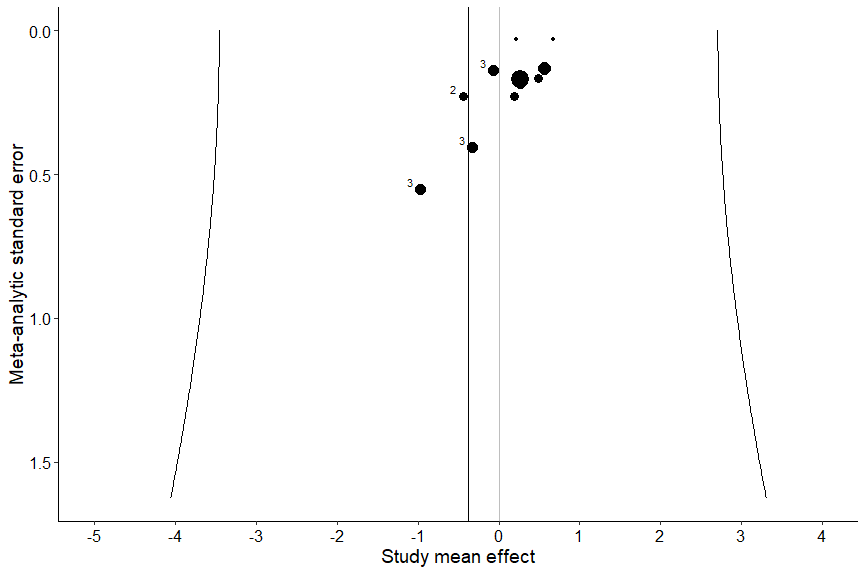
\includegraphics{images/funnel_study.png}

Again, the overall effect size is the vertical line to the left of zero. We want to see symmetry around that line, vertically and horizontally. But again, we don't. Interesting!

\hypertarget{reporting-publication-bias-1}{%
\subsubsection{Reporting Publication Bias}\label{reporting-publication-bias-1}}

Ok, so we've now looked at two different funnel plots to check for publication bias. What do they tell us, and how do we report it? Well, we know the funnel plot was not very symmetrical. This means that publication bias may be a concern in our sample. Unfortunately, to the best of my knowledge in January 2024, we can't quantify this as well with three-level models as we can with conventional meta-analysis.

\hypertarget{thats-it-1}{%
\section{That's it!}\label{thats-it-1}}

You've now gone through all the steps needed to conduct a three-level meta-analysis. Congratulations! This may seem intimidating, but if you complete each step, in order, this will be a very simple process. And think - now you a) have a code you can adapt and use for every three-level meta-analysis you conduct in the future, b) have a code you can share with friends, and c) can share you code with your publication so others can replicate your analysis. Just think - if more people had done that I would not have had to write this book\ldots.

\hypertarget{section-1}{%
\subsubsection{}\label{section-1}}

\hypertarget{part-notes}{%
\part{Notes}\label{part-notes}}

\hypertarget{change-log}{%
\chapter*{Change Log}\label{change-log}}
\addcontentsline{toc}{chapter}{Change Log}

February 6, 2024: Book made available online.

  \bibliography{references.bib}

\end{document}
